%%% Local Variables:
%%% mode: latex
%%% TeX-master: t
%%% End:

\documentclass[doctor,openright]{tongjithesis}
% \documentclass[%
%   master|doctor, % mandatory option
%   xetex|pdftex|dvips|dvipdfm, % optional
%   secret,
%   openany|openright,
%   arialtoc,arialtitle]{tongjithesis}

% % 所有其它可能用到的包都统一放到这里了,可以根据自己的实际添加或者删除。
\usepackage{tongjiutils}
\usepackage[top=2.54cm, bottom=2.54cm, left=3.17cm, right=3.17cm]{geometry}
%\newcommand{\citeA}[1]{\citeauthor{#1}, \citeyear{#1} \cite{#1}}
%\newcommand{\citeB}[1]{(\citeauthor{#1}, \citeyear{#1} \cite{#1})}

% 你可以在这里修改配置文件中的定义,导言区可以使用中文。
\def\myname{邱君诚}

\begin{document}

% 定义所有的eps文件在 figures 子目录下
\graphicspath{{figures/}}


\frontmatter

%%% Local Variables:
%%% mode: latex
%%% TeX-master: t
%%% End:
\secretlevel{保密} 
\secretyear{2}

\ctitle{基于弹性波模式解耦的全波形反演方法}

% 按照申请工学学位设计。如有其它需要,请修改相应文字。
\makeatletter
  \iftongji@doctor
    \cdegree{博士}
  \else
    \iftongji@master
      \cdegree{理学硕士}
    \fi
  \fi

\makeatother

\cdepartment{同济大学海洋学院}

\cmajorfirst{固体地球物理}

\degtype{理学}

\cauthor{王腾飞}

\cstnr{1110701}

\csupervisor{程玖兵 教授}

% 如果没有副指导老师或者联合指导老师,把各自{}中内容留空即可。

\cassosupervisor{}

\ccosupervisor{}

% 日期自动生成,如果你要自己写就改这个cdate
%\cdate{\CJKdigits{\the\year}年\CJKnumber{\the\month}月}
\makeatletter
  \iftongji@doctor
    \edegree{Doctor of Philosophy}
  \else
    \iftongji@master
      \edegree{Master of Science}
    \fi
  \fi

\makeatother

%\cfunds{自然基金项目(No.123456789)}

%\efunds{(Supported by the Natural Science Foundation of China for\\ Distinguished
%         Young Scholars, Grant No.123456789)}

\etitle{Elastic Full waveform inversion based on wave mode decomposition}

\edepartment{School of Ocean and Earth Science}

\edispline{Natural Science}

\emajorfirst{Solid Geophysics}
%\emajorsecond{TONGJILUG}

\eauthor{Tengfei Wang}

\esupervisor{Prof. Jiubing Cheng}

%\eassosupervisor{Prof. Gang Wan}

% 这个日期也会自动生成,你要改么?
% \edate{May, 2009}

% 定义中英文摘要和关键字
\begin{cabstract}
	弹性波全波形反演方法(EFWI)想要通过最小化实际观测到的多分量数据与正演模拟的数据
	之间的残差来获得高分辨率的地下参数模型。由于Hessian矩阵的显式计算与反演代价十分
	巨大,大规模的应用问题通常采用梯度类的最优化方法而非基于Hessian的方法。然而多参数
	反演中,参数耦合效应会引起不同参数间梯度的串扰,进而会严重影响反演过程的速度与精度。
	近期以来,弹性波模式解偶的方法被用来对梯度进行预条件从而降低EFWI过程中的参数耦合
	问题。在本文中,我们提出了一种基于模式解偶(MD)的EFWI方法,该方法在时间域通过正传
	与解偶的反传波场之间的互相关来获得梯度。基于解偶的Frech$\acute{e}t$导数,我们通过分析
	Hessian矩阵和分辨率矩阵、对比Gauss-Newton梯度来解释本方法的物理机制。简单流体饱和模
	型与Marmousi-II模型的数值实例,证明了基于MD的预条件共轭梯度法可以降低P-波和S-波速度
	之间的参数耦合,并且在不涉及Hessian计算的同时获得快速的收敛。
\end{cabstract}

\ckeywords{\TeX, \LaTeX, CJK}

\begin{eabstract}
Elastic full waveform inversion (EFWI) aims to reduce the misfit between recorded and modelled multi-component
seismic data for deducing a detailed model of elastic parameters in the subsurface.
Because the explicit computation and inversion of the Hessian matrix
is extremely resource intensive,
a gradient-based (rather than Hessian-based) minimization is generally applied for large-scale applications.
However, the multi-parameter trade-off effects cause cross-talks in the computed gradients and
thus severely affect the convergence and the quality of the inverted model.
Recently, preconditioning the gradients based on elastic wave mode decomposition
has been suggested for mitigating the parameter trade-offs in the EFWI process.
In this paper, we propose a mode decomposition (MD)-based EFWI approach, in which the preconditioned gradients
are obtained through the cross-correlation of the forward and
decomposed adjoint wavefields in the time domain.
Based on the decomposed Frech{$\acute{e}$}t derivatives,
we explain the mechanism of this approach through analyses of Hessian and resolution matrices
and comparisons with the Gauss-Newton gradients.
Numerical examples of a simple fluid-saturated model and the Marmousi-II model
demonstrate that the MD-based preconditioned conjugate-gradient approach
can mitigate the trade-off between the P- and S-wave velocities and achieve fast
convergence without any Hessian-involved calculations.
\end{eabstract}

\ekeywords{Waveform inversion, Elasticity, Mode decomposition, Resolution matrix
}

\makecover


% 目录

\tableofcontents

\include{data/denotation}

%\listoffigures

%\listoftables

%\listofequations

%%% 正文
\mainmatter
%\chapter{引言}
\section{研究背景和意义}
地震勘探的终极目标是通过观测到地震数据来定量地估计地下模型。
弹性参数,包括纵(P)波速度,横(S)波速度以及密度等等物性参数可以通过岩石物理来定量的估计岩石物理参数,从而获得储层及其围岩的岩石性质。这对油气的开发,油田
监测以及CO$_2$注入等具有重要意义。传统的常规地震数据处理中,通常用声波方程来描述地震波在地下介质中的传播。而地下介质的真实模型往往要复杂得多,需要通过弹性
各向同性、具有垂直(水平)对称轴的横向各向同性(VTI,HTI)、正交各向异性(ORT)、衰减等等来更准确的描述波传播。但是模型假设越复杂,所引入的计算量也越大,
而所对应的多参数反问题也越困难。目前来看从声介质过渡到弹性介质能够以较小代价来获取较准确的模型近似。
尽管如此,从声波近似过渡到到弹性假设也会成倍地增加计算量,但是采用弹性波假设来进行成像或者反演仍然十分必要。因为考虑弹性假设的数据处理流程能区分数据中的
P波与S波模式,从而获得更多与岩性相关的信息,这对于岩性估计、流体识别、气云成像、裂缝与应力刻画以及密度估计都非常重要。
近年来,非常规油气藏,如致密页岩气(油)等开发技术极大地依赖于岩石物理参数的估计,这使得考虑弹性介质甚至各向异性假设都需要提上日程。

地震勘探中的诸多技术都非常依赖于速度模型的精度。
因此在众多物性参数中,如何获取准确的高分辨率速度模型是地震勘探中最为迫切的任务。
为了降低地震数据与模型描述之间的非线性程度,Claerbout(1985)\cite{Claerbout1985Imaging}在其书中将速度模型分解为两个部分:1)描述速度(阻抗)界面的高频部分;
2)描述波传播走时的低频部分。这样的分解方式分别对应于地震勘探中最核心的两个任务,也即偏移成像与速度建模。传统方法中偏移成像+AVO/AVA
技术通常用来获取模型的高频部分,
而偏移速度分析(MVA)和层析技术被用来恢复模型的低频部分。但是这类方法所能恢复的波数谱上存在明显的间断区域,正如著名的图\ref{fig:GapInSeisVel}
所示(选自Claerbout(1985)\cite{Claerbout1985Imaging}),速度模型的中低成分波数很难恢复。这就需要引入旨在恢复全频带速度信息的FWI方法。
而随着高性能计算能力的不断提升,基于波动理论来获取模型高、低波数成分的方法也受到了广泛关注。
\begin{figure}[!htb] 
   \centering 
   \subfloat[]{\includegraphics[width=0.68\textwidth]{Figure/chapter01/GapInSeis.jpg}}
   \caption{Vertical profiles of elastic WERTI and EFWI results at 1.4km (a) and
       3km (b). The black and blue lines indicate the true and linearly         increased
       initial model. The green and yellow lines indicate the WERTI and EFWI    results,
       respectively.
   }
   \label{fig:GapInSeisVel}
\end{figure}

传统常规方法中大多基于射线类方法进行成像与速度估计,这在模型复杂区域很难处理多路径以及焦散等问题。而基于波动方程的方法则可以避免上述问题。
目前基于波动理论的主要反演方法主要有以下三类:

1、FWI,该方法通过匹配数据中携带的所有信息,包括走时、振幅、模式转换、多次波等等,来获得对地下模型的全波数谱的
恢复。
相比走时反演和MVA,它可以获取更高分辨率的地下模型。
因此自从Lailly(1983)\cite{lailly1983seismic}和Taratola(1984)\cite{tarantola1984}建立了FWI理论框架之后,随着宽频带,宽方位数据采集的成熟,FWI
被认为是填补速度模型中尺度波数成分空白的最强有力的工具。
但是FWI也受到众多的制约,如强烈的非线性程度(cycle-skipping),数据不完备导致的有限观测孔径,地下实际介质的非弹性以及各向异性,计算代价十分昂贵等等,因此
FWI虽经过数十年发展所面临的挑战依然十分艰巨;

2、波动方程偏移速度分析(WEMVA),该类方法旨在更新模型中的长波长背景速度,也即模型的低波数成分。
目前主流的做法通常利用数据中的反射波信息,通过获取反射波波路径信息来获得模型中深部的速度更新。
而根据其目标函数的残差类型又可以分为数据域反演(如Xu et al., 2012\cite{xu:2012};Wu and Alkhalifah, 2015\cite[]{Wu2015}; Zhou et al, 
2015\cite[]{zhou:2015}; Chi et al, 2015\cite{chi:2015})和扩展成像域反演(如Sava和Fomel, 2006\cite{Sava2006}; Almomin和Biondi, 2012\cite{Almomin2012})。
此类方法与基于射线理论的成像域层析与数据域(非线性)层析方法一脉相承,但是避免了传统层析流程中繁琐的人工拾取工作,不过其同样也会受困于cycle-skipping等问题;

3、最小二乘逆时偏移(LSRTM),该方法可以看作是线性化的FWI,在初始模型足够好的时候通过匹配模拟数据与观测数据的振幅来获得地下反射系数模型。常规偏移成像
采用伴随算子来近似正传算子的伪逆,从而近似地获得反射率的成像结果。但是伴随算子通常近似效果很差,最小平方偏移(LSM)通过迭代方式来获取正传算子的伪逆从而获得
更好的成像效果((Nemeth et al., 1999,Kühl and Sacchi, 2003,Dai, 2012)。该过程可以看作是对目标函数对模型的二阶导数,也即Hessian,近似求逆的过程。

结合以上背景,如何恢复弹性介质中的速度模型将对勘探地球物理的发展至关重要。将弹性假设引入到以上反演问题中将会大大增加反问题的非线性程度。同时,多参数反演
也会带来参数间的耦合效应,这会进一步增加反演难度。由于计算机能力提升、多分量观测数据的增多以及解决声波FWI无法回避的问题的需要,考虑弹性甚至各向异
性的全波形反演逐渐成为研究热点。弹性波多分量数据中同时含有P波和S波,这两种不同波模式对地下介质有着不同的刻画作用。
近年来弹性波波模式分离技术能够提供准确的P或S波数据子集,这对反演中采取更多的多尺度策略带来可能性。在反演过程中,不同参数采用不同的数据子集或者不同的反演阶段
采用不同的数据子集,这将大大降低法多参数反演的非线性程度,同时也可以回避参数间的耦合效应。在本文中,这种策略将贯穿始终,
模式解耦将在EFWI,弹性波波动放程反射走时反演(EWERTI)以及E-LSRTM中提供的分离的P或S波数据,来帮助获得更好的反演结果。
\section{研究现状}
\subsection{弹性波FWI研究现状}
Claerbout(1971\cite{Claerbout1971})采用爆炸发射面的概念解释了成像条件可以通过多次叠加来对地下构造进行刻画。Lailly(1983\cite{lailly1983seismic})
和Tarantola(1984\cite{tarantola1984})最早引入了表示观测数据与模拟数据间波形残差的$L_2$目标函数,将这种偏移成像的原理重新转化为寻优的
最优化问题,也即FWI。而该最优化问题的梯度方向可以采用共轭状态法求取,通过入射波场与反传波场之间的互相关来获得。FWI试图将速度宏观模型的恢复(速度
建模)与偏移成像两个任务统一在一个流程中,这样就可以在地下每个网格点获得具有连续波数谱的高分辨率结果。但是早期只利用反射数据的FWI很少有令人满意的
结果,因为短偏移距观测的地震数据对中尺度波长的模型信息非常不敏感(Virieux和Operto(2009)\cite{virieux2009overview}),这就需要在初始模型非常准确
的时候FWI才能获得收敛。
从上世纪80年代末期,随着FWI在长偏移距以及井间透射波的应用成功,人们才发现FWI的潜力(Mora, 1987\cite{mora:1987}, 1988\cite{mora1988elastic}; Pratt
and Worthington, 1990\cite{PRATTEtAl1990}, Pratt et al., 1996\cite{pratt1996two})。
近年来在长偏移距、宽方位和宽频带采集的数据逐渐增多后,基于声波近似的FWI也在越来越多的实际数据中获得成功应用,例如Ravaut
et al., 2004\cite{RavautEtAl2004},Operto et al., 2006\cite{Operto2006},Shinet al.,
2009\cite{ShinEtAl2009}。然而即使对于含有长偏移距的数据而言,由于波传播路径的增加,非线性程度变得更加剧烈,因而从FWI中获得稳健的反演结
果仍然受到很大挑战\cite{sirgue2006importance,virieux2009overview}。

而从前文背景分析可以知道,最早始于Tarantola(1986)\cite{tarantola:1986}和Mora(1987)\cite{mora:1987}的弹性波全波形反演能够从多分量数据中反演地下介质的弹性参数,如P/S-波速度和密度。
尽管其仍然需要很大计算代价,EFWI还是在很多实际数据中获得了应用
\cite{crase1992nonlinear,djikpesse.tarantola:1999,sears:2008,sears:2010,prieux:2013a,prieux:2013b,vigh:2014}。
EFWI的实现方式可以在时间域\cite{shipp:2002},可以在频率域\cite{brossier2009},也可以采用混合的方式在时间域进行正演模拟而在频率域求解
\cite{nihei.li:2007,sirgue:2008}。然而,EFWI中多个参数参与反演会增加反问题的非线性程度,同时也会受到由于不同物理参数之间的串扰带来的反演
中参数耦合的影响\cite{forgues.lambare:1997}。在海洋环境中,尤其是在软海底环境中,由于P-to-
S的转换模式非常弱,基于拖缆或者海底多分量数据的EFWI的非线性程度会变得更严重\cite{sears:2008}。

从声波介质到弹性介质,波形反演方法将受到诸多挑战,解决EFWI中的问题,不仅要应对原有声波框架下的困难,同时也要解决多参数反演带来新问题。总的来说,
EFWI将主要面临以下两个方面的挑战:

1、反演的非线性,也即Cycle-skipping。FWI是基于Born近似的理论框架导出的。在Born散射下,Miller et al\cite{miller:1987}基于ray+Born理论,
导出模型中散射点局部的波数矢量可以表达为:
%\begin{equation}
$    \mathbf{k}=\mathbf{k_s}+\mathbf{k_r}=\frac{\omega}{v}cos\frac{\theta}{2}\mathbf{n}$。
%    \label{eq:Modelwnb}
%\end{equation}
其中$\mathbf{k}$为照明矢量,$\mathbf{k_s}$和$\mathbf{k_r}$分别是震源端和检波点端的波场波数矢量,$v$为局部速度,$\theta$为散射角,
$\omega$为角频率,$\mathbf{n}$为$\mathbf{k}$方向的单位向量。由上式可以看出,低频和大孔径($\theta$)数据对于中低波数成分的恢复至关重要。
\begin{figure}[!htb] 
   \centering 
   \subfloat{\includegraphics[width=0.40\textwidth]{Figure/chapter01/Wavenumbervector.pdf}}
   \subfloat{\includegraphics[width=0.40\textwidth]{Figure/chapter01/Cycle-skipping.pdf}}
   \caption{Vertical profiles of elastic WERTI and EFWI results at 1.4km (a) and
       3km (b). The black and blue lines indicate the true and linearly         increased
       initial model. The green and yellow lines indicate the WERTI and EFWI    results,
       respectively.
   }
   \label{fig:WavenumberVector}
\end{figure}
因此FWI的成功与否非常依赖于长偏移距记录和数据中有效的低频分量。如图\ref{fig:WavenumberVector}b
所示,如果初始模型不够好导致波形匹配时相差$\frac{1}{2}T$以上,那么就会使得反演陷入局部极值,这也就是所谓的“周波跳跃”问题。
在声波FWI中,发展了许多策略来解决非线性问题,如从低频到高频(Sirgue and
Pratt, 2004\cite{sirgue.pratt:2004}; 刘国峰等, 2012\cite{刘国峰2012};
刘璐等,2013\cite{刘璐2013}; 曹书红和陈景波, 2014\cite{曹书红2014}; 
张文生等, 2015\cite{张文生2015}),选取不同的时窗与偏移距逐步加入反演中(Shipp and
Singh, 2002\cite{shipp:2002}; Wang and Rao, 2009\cite{WangEtAl2009}; Sears,2008\cite{sears2008}),
修正目标函数使其凸性更好(Luo and Schuster, 1991\cite{luo1991};Tromp et al.,
2005\cite{tromp2005seismic};Chi
et al., 2014\cite{ChiEtAl2014}; Wu et al., 2014\cite{Wu2014b}; Shin and Cha,
2008\cite{shin.cha:2008}; Luo et al., 2016\cite{Luo2016})等等。这些策略可以用
在EFWI中,但是由于更多参数引入以及更复杂的弹性波波场,使得在使用这些策略的时候需要根据情况来择优选取。
而在EFWI中,不但会出现同样的强烈非线性,而且将面临更复杂的情况。
在构建初始模型的时候我们要同时获得足够好的$V_p$与$V_s$模型,这样才能对各种模式的转换波形进行
匹配。而$V_s$模型相比$V_p$初始模型更难获得。目前许多EFWI研究中都假设了$V_s$与$V_p$之间有着固定的Poisson's比值的关系,因此可以通过简单的系数相乘
来构建初始模型。但是当地下介质Poisson's比变化较大时很难获得较好的$V_s$初始模型,这就又增加了EFWI的困难。为了降低弹性波FWI非线性程度,许多学者通过
包络目标函数(黄超等,2015\cite{黄超2015},王官超和杜启振,2016\cite{王官超2016}),或者通过研究目标函数性态来指导多尺度策略的设计
(Brossier et al., 2010\cite{BrossierEtAl2010};王毓玮等,2016\cite{王毓玮2016})。
Tarantola(1986)\cite{tarantola:1986}指出EFWI应分主次顺序依次构建具有不同影响的参数。
或者采用多尺度策略多级的选取不同数据分量来进行反演(Sears, 2008\cite{sears2008}; Operto et al., 2013
\cite{operto2013guided})。然而实际中,诸多因素会制约这些策略的应用,例如(低频缺失,初始模型不够好,子波估计,噪音等等)。因而降低EFWI的非线性
程度使得反演更加稳健可靠依然需要诸多努力。

2、多参数反演中的参数耦合效应。如果物理模型中引入多个参数,那么不同的参数扰动可能会引起类似的数据扰动。虽然其产生的数据扰动可能不完全一致,
但是不同参数的“偏导数波场\cite{pratt1998gauss}”会在特定角度范围内的重叠,这就导致无法简单地区分开数据扰动来自哪一种
参数扰动,从而引起参数间的耦合效应。这样的话,即使在初始模型足够好的时候也很难从数据扰动中恢复其相应的参数扰动。为了解决EFWI中的参数耦合问题,
许多学者通过调查散射模式或者Hessian算子来选取不同的参数化方式(Wu and Aki, 1985\cite{wu.aki:1985};Tarantola, 1986\cite{tarantola:1986};
Plessix and Cao, 2011\cite{plessix.cao:2011},Gholami et al, 2013\cite{gholami2013})。
当然最有效的就是考虑多参数Hessian算子的方法,用Hessian的信息来压制参数耦合的影响(Fichtner et al., 2001\cite{fichtner2011hessian};Operto et al.,
2013\cite{operto2013guided},Pan et al., 2015\cite{pan2015estimation};Yang et al.,
2016\cite{Yang2016})。然而由于Hessian计算所需代价太过于昂贵,即使在声波FWI也很难在大规模问题中获得应用。在EFWI中想要获得压制参数耦合的效果,就
需要在反演中包含对Hessian的非对角区块的近似。近期,在Hessian非对角区块的近似与利用方面,许多学者都将其应用到了EFWI中,例如Wang
et al.(2016)\cite{WangEtAl2016}采用块对角Hessian压制参数耦合,Pan et
al(2017)\cite{PanEtAl2017}采用Hessian-free的方式采用l-BFGS的优化策略进行多参数反演,Wang and Cheng
(2017)\cite{WangEtAl2017}指出模式解耦可以部分的利用Hessian非对角块来压制P波对$V_s$反演的干扰。而于此同时EFWI中,由于密度参数对数据不敏感,因此密度
的反演依然很难获得令人满意的结果。
\subsection{弹性反射波FWI研究现状}
尽管常规FWI在长偏移距,宽方位数据中有着令人满意的效果,但是在这种观测系统下,FWI主要利用了长偏移距透射波以及临界反射波所携带的信息来更新速度模型的
中长尺度波长的分量。由于FWI的成功非常依赖这种透射信息,就会使得FWI往往缺乏足够的大偏移距信息来更新模型中深部结构的中低波数成分。
这就导致在深部的区域,FWI往往只能更新来自反射数据的高波数成分(也即是最小平方偏移的过程)而很难更新中低波数成分。从图\ref{fig:WavenumberVector}
中也可以看出,在相同频率和速度下,深部的反演需要更大的角度覆盖才能确保足够的低波数照明,这也意味着要更大的偏移距。然而即使对
于目前宽方位长偏移距的采集技术也很难保证这样的覆盖,况且更长的偏移距也意味着更强的非线性\cite{sirgue2006importance,virieux2009overview}。

利用反射波信息可以更好的照明深部,通常可以在成像域或者数据域实现深部的速度更新。在成像域,该类方法通常被称为偏移速度分析(MVA),其主要利用拉平
共成像点道集作为收敛准则。
在实际生产中,通过射线走时层析来利用反射波信息更新中深部的背景速度已经是非常成熟的技术\cite{Woodward1992,MengEtAl2004, Woodward2008,
Jones2010}。其通过将道集上的剩余时差(或深度差)反投影到射线路径上来获得速度更新。不过射线层析经常需要进行许多人工干预,尤其是在每轮迭代中进行
成像剖面与成像道集的拾取。而且在构造复杂区域,射线高频渐近近似失效,使得走时层析很难获得成功。
基于波动理论的成像域偏移速度分析(WEMVA)可以很好的回避上述问题,但是其通常
需要引入扩展成像条件,通过最小化扩展道集上非零偏移距的能量来实现更新,如Sava and
Fomel(2006)\cite{SavaEtAl2006}; Yang and Sava(2011)\cite{YangEtAl2011}; Almomin and
Biondi(2012)\cite{Almomin2012}; Sun and Symes(2012)\cite{SunEtAl2012}。尽管WEMVA在
二维应用中取得了不错的效果,但其主要缺陷就是计算代价太过昂贵,尤其实在三维问题中,一方面偏移成像需要大量计算,
另一方面扩展成像条件的施加同样耗费极大。
针对反射走时,Luo et
al(2016)\cite{Luo2016}用时间轴方向的扩展成像与Rytov近似结合,导出了全走时反演(FTI)获得了不错的反演效果,但其实质上也是一种成像域的反演方法。

在数据域同样可以实现反射波对模型的深部更新。
许多学者(Chavent et al, 1994\cite{ChaventEtAl1994}; Plessix et al.,1998\cite{PlessixEtAl1998}; Clment et al.
,2001\cite{ClementEtAl2001})将速度模型分成高波数(反射率)与低波数成分(背景模型),提出了偏移成像走时层析(MBTT)。
从Woodward et
al.(2008)\cite{Woodward2008}和Alder(2008)\cite{Adler2008}提出的基于射线理论的非线性层析方法出发,Wang
et al\cite{WangEtAl2014}和Yang et al\cite{YangEtAl2016}采用一次偏移后拾取+图偏移的方式建立叠前数据的不变量(如走时,相位,出射慢度等),从而实现对
叠前数据的多次非线性拟合,进而减少人工拾取工作量达到加快速度的效果。基于波动理论的数据域速度建模近年来受到了广泛的关注。
受MBTT方法的启发,Xu et al (2012)\cite{xu:2012}提出了反射波波形反演方法(RWI)。RWI先采用RTM或LSRTM的方式获取反射率,
然后用Born模拟来预测反射率所产生的反射波,而反射波与背景波场的互相关就可以得到反射波波路径信息。
RWI思想的关键就是将数据域中通过不同目标函数获得的数据残差反投影到反射波波路径上,从而更新中低波数成分的模型分量。
RWI的思想产生后,许多学者针对不同的目标函数选取方法做了很多研究。许多RWI研究都采用波形拟拟合的$L_2$范数,如Xu
et al (2012)\cite{xu:2012}, Wang et al(2013)\cite{Wang2013}, Wu and
Alkhalifah(2015)\cite{Wu2015b},
Zhou et al(2015)\cite{zhou:2015}。然而尽管RWI的目的在于更新背景速度,波形拟合的$L_2$范数在背景速度与真实值相差较远的时候,反射率所预测的反射波与
观测数据中的反射波波形相差半个周期以上的时候,仍然会产生周波跳跃。Wang et
al(2013)\cite{Wang2013}指出采用低频数据可以一定程度上避免跳周现象。为了避免振幅相关的目标函数带来的非线性,与背景速度更具有线性关系的
走时类的目标函数也获得了关注。Ma and
Hale(2013)\cite{ma2013}采用动态图像识别(DIW)来获得模拟与观测反射数据之间的时移,从而导出了波动方程反射走时反演(WERTI)。Chi
et al (2015)\cite{chi2015}和Wang et al
(2015)\cite{Wang2015}采用互相关类的方法来获取时移(或空移)。而近期,Irabor and
Warner(2016)\cite{Irabor2016}和Wang et al(2016)\cite{WangEtAl2016}通过上下形波分离来获取常规FWI中的背景更新分量,但其实质上也利用了反射波波路径的信息。

以上RWI的研究现状都是基于声波方程得出的。在弹性波反射波形反演中,目前只有Guo and
Alkhalifah(2016)\cite{Guo2016}将Wu and
Alkhalifah(2015)\cite{Wu2015b}的思路扩展到了弹性介质中,而其他方法在弹性介质中的应用则
基本没有研究触及到。在弹性介质中,除了声波介质中面临的问题,ERWI还需要处理更多的复杂情况,如多参数,模式转换,更复杂的反射记录以及
$V_s$结构中成像与反演的困难等等诸多挑战。为了解决这些问题,利用波模式解耦来分别获取P与S反射波然后应用到声波对应的方法中将是非常直观的思路,但是
这都需要考虑到弹性波的特殊情况,处理好每种方法相应的问题才能获得可行的ERWI方案。
%许多研究通过选取不同的目标函数来选取方法对应不同名称的反演方法,但核心思想都是一致的

\subsection{弹性波LSRTM研究现状}

目前有许多成像方法,如Kirchhoff偏移,高斯束偏移,RTM等等可以用来恢复地下界面结构。但是随着技术进步,界面构造信息已经不能满足勘探的需要,我们想要
获得更准确的高波数成分。
常规的FWI算法可以高分辨率地恢复模型的高波数成分,但是会受到许多因素干扰,
如cycle-skipping问题,信噪比低,地震子波未知,正演算子不准确等等。
而且常规FWI需要从低频到高频逐步恢复连续的波数谱,如果我们单纯想获得模型高波数成分,
用FWI方法就太过复杂。除FWI之外,我们通常也会通过最小平方偏移(LSM)来实现高波数成分的重构。
早期,Beylkin(1985)\cite{Beylkin},Bleistein,
1987等学者通过广义Radon变换来导出Kirchhoff成像中的振幅校正因子,也即真振幅成像技术。该方法通过射线理论计算Green函数,正问题采用Born近似
计算,进而快速的迭代求解反问题。
针对Kirchhoff偏移,Schuster(1993)\cite{Schuster1993}提出了应用于井间数据的LSM算法,而Nemeth et al.\cite{Nemeth1999}将该方法应用到了地面数据中。
以波动方程为引擎的最小平方逆时偏移(LSRTM)近年来一直是研究的热点,
尽管其计算代价昂贵,但是LSRTM可以回避模型速度复杂时所产生的多路径问题。
LSRTM的过程通常被认为是线性的全波形反演,理论上施加Hessian矩阵的逆就可以获得最终的反演结果。但是Hessian的计算与求逆在实际问题中基本无法实现,
在空间域采用Hessian的近似来校正成像结果是一种快速获得LSRTM结果的方法\cite{ChaventEtAl1999,shin2001improved,Symes2008},然而这种方法在复杂区域并
不总是有效。另外一种方式是通过在数据域求解目标函数的最优化问题其假设在已经获得足够好的低波数模型成分之后恢复模型的高频扰动,也即获得“像”或
反射率,使得在最小平方意义下,用该反射率所预测的反射数据能与观测数据达到最佳匹配。这一过程与在单次迭代中通过计算二阶伴随状态方程来使用
Gauss-Newton法(Bae et al., 2012\cite{bae2012frequency};Metiver et al.,
2014\cite{Metivier2014})求解FWI是一致的。
因此,最小平方逆时偏移与全波形反演的理论框架是一致的,只是输入数据(反射波与全波场)和输出结果(高频扰动与模型参数)不一样。
因此目前LSRTM研究的主要方式通过最小化Born模拟的反射数据与观测数据之间的残差来改善成像质量、获得更高分辨率的结果(Dai and
Schuster(2013)\cite{Dai2013},Dong et al.(2012)\cite{Dong2012}, Luo and
Hale(2014)\cite{Luo2014})。

许多学者针对LSRTM中的不同问题做了大量的研究工作。Wong et al.
(2015)\cite{WongEtAl2015}将自由表面多次波加入到成像条件中,进而增加地下照明。Zhang et al.
(2015)\cite{ZhangEtAl2015}选取零延迟互相关目标函数来减弱子波估计不准以及振幅描述不准带来的非线性。刘玉金和李振春
(2015)\cite{刘玉金2015}基于成像域的速度反演方法(Symes,2008\cite{Symes2008a})
在扩展域进行LSRTM,这样即使在速度不准确的情况下仍然可以得到合理的成像结果。
近期,为了更准确地描述波传播过程,同时获得更多的参数成像,并解决多参数带来的耦合效应,原本基于声波方程的
LSRTM被推广到了变密度声波介质(Yang et al, 2017)\cite{Yang2017}),衰减介质(Dutta and
Schuster, 2014\cite{DuttaEtAl2014}; 李振春等,2014\cite{李振春2014}; Dai et al,.
2015\cite{Dai2015})以及弹性介质中(Duan et al., 2016\cite{Duan2016};Feng and Schuster,
2016\cite{Feng2016}; Xu et al., 2016\cite{Xu2016};Ren et al., 2016\cite{RenEtAl2016})。

相比声波成像,弹性波成像可以提供更多的地下信息,例如裂缝分布以及弹性性质。但是,弹性波偏移中存在的许多问题会很大程度上影响成像质量。因为通常很难将记录中的
波模式完全区分开,因此其中某些波模式的会因速度不对而被错误地成像。这些非物理的模式就会引起假象,也即“cross-talk”。
而通过ELSRTM则可以提高成像的分辨率,并且可以压制由于观测孔径限制,粗网格采样以及数据缺失引起的偏移假象。
弹性波成像面临处理多分量数据的问题,也就需要选取合适的成像条件,{\color{red}\cite{Wang2016}提出了无极性反转的矢量成像条件。}而从EFWI理论框架出发,许多学者,
如Duan et al.(2016)\cite{Duan2016},Feng et
al.(2016)\cite{Feng2016}等都推导出了与EFWI梯度非常类似的成像条件。该成像条件也可以回避极性反转问题,同时也可以认为是更加接近于高频的参数扰动梯度。
\section{研究内容}
弹性介质中参数的恢复与重构将是本文的重点。
为了估计弹性介质中的模型参数,现有的最有潜力的方法需要从声波模型扩展到弹性介质模型中,包括FWI、RWI和LSRTM。
我们将以上三个方法扩展到弹性介质来研究与估计模型参数,其非别对应为EFWI构建高分辨率速度模型,E-WERTI构建中深部中低波数的背景速度,
E-LSRTM构建模型高波数成分。而整个论文中,弹性波模式解耦将贯穿始终,来为每种方法提供不同的数据子集以及降低参数耦合的便利。
因此本论文将分为以下四个部分来详细阐述:

第二章中,我们通过模式解耦来对EFWI梯度进行预条件来降低反演过程中的参数耦合程度,并达到加速收敛的效果。
首先,通过弹性波Born近似,我们分析了P波速度与S波速度扰动的
辐射模式,并导出了解耦的Frech{$\acute{e}$}t导数或Jacobian矩阵;然后,我们调查了解耦后的P波与S波数据对梯度的贡献并提出了在梯度计算中的交叉项近似。
在此基础上,预条件的梯度可以通过伴随状态法\cite[]{plessix2006}快速有效地计算得到,也即正传波场与解耦后反传波场的零延迟互相关。
然后,为了获得更多物理机制上的认识,我们计算并分析了基于解耦的Hessian和分辨率矩阵,同时也比较了MD预条件后的梯度与GN梯度的异同。
此后,我们通过在流体饱和沙岩模型以及Marmousi-II模型的数值实验证明了基于解耦的EFWI的有效性。
最后,我们给出关于密度反演的简单讨论并获得了一些结论。

第三章中,我们将通过弹性波波动方程反射走时反演(E-WERTI)来重建速度模型中深部的中低波数分量。
文中采用走时作为目标函数进行反演,反射波的走时差将通过DIW来获取。
我们采用RWI的思路通过Born模拟来构建反射波关于背景速度的核函数,也即反射波波路径。
由此我们参照Ma and Hale\cite{ma2013}来导出弹性波方程对应的反射走时反演梯度与伴随震源。
在文中,我们首先通过目标函数的形态分析调查了E-WERTI的稳健性与收敛性。然后通过反射核函数的分析观察了不同反射波波模式对反射路径的影响。
为了克服P波与S波速度之间的耦合性,我们将分成两个阶段来分别恢复P波与S波速度。两个阶段中,我们将用地面分离+波场分解的方式来获取分离后的P或S
波对应的多分量地面数据以及地下的波场。由此,我们先采用PP波反射走时来重构出P波速度的背景模型,在获得足够的P波背景速度后,固定P波速度背景模型,
采用分离出的PS波反射信息来重构S波速度背景模型。最后我们将算法在Sigsbee2A模型上进行试验。

第四章中,我们采用弹性波LSRTM来获取模型的高波数分量。首先,我们从反演框架出发,建立模拟与观测反射数据之间的最小二乘目标函数,
利用弹性波Born近似通过Lagragian乘子法导出E-LSRTM的梯度。之后我们根据第一章的推导,利用波模式解耦思想对导出的梯度进行预条件来降低参数耦合效应。
由于LSRTM为线性FWI过程,反问题的复杂程度将大为降低,因此我们将对比不同的策略来解决参数耦合问题。最后将根据简单模型实验结果设计最优的E-LSRTM
反演策略。简单模型与Marmousi的数值实验将用来验证算法。
由于梯度的推导基于Born近似,我们将先利用Born正演数据来检验算法,然后采用更接近实际问题的
正演反射数据来进行实验。

第五章中,将对本文的工作进行总结,讨论论文的创新与不足之处,并规划下一步的研究重点。

%
%%% Local Variables:
%%% mode: latex
%%% TeX-master: t
%%% End:



\chapter{弹性波模式解耦全波形反演}
\label{cha:MD-EFWI}
\section{引言}
针对地下介质的定量成像方法对于定位与刻画油气储层、监测CO$_2$注入以及估计近地表土壤和岩石的物理性
质非常有必要。相比于从地震偏移获得的定性化的叠后反射系数,人们更希望得到定量化的深度域弹
性参数。地震反演旨在采用迭代优化类方法通过拟合正演数据与实际观测数据来恢复地下的参数模型。
与仅利用走时信息的层析反演方法不同,例如Luo and Schuster (1991)\citep{luo1991},FWI提供
了更加完善的思路,同时利用走时与振幅信息来反演参数模型\cite[]{tarantola:1986}。
随着长偏移距、宽方位和宽频带采集技术的应用,全波形反演已经成为构建高质量速度模型和进行定量地震成像的有效工具\cite{virieux2009overview}。

然而,FWI有许多制约因素。首先,它所需计算量十分巨大,尤其是在三维模型反演中。尽管梯度类的局部优化方法并不能保证反演收敛到全局最优解,
但为了降低计算代价仍然被广泛应用于FWI中。收敛性更好的基于Hessian的反演方法\cite{mora:1987,crase1990robust}
因其更昂贵的计算代价则更多被FWI所舍弃。此外,为了减少计算量,人们通常采用声学近似来获得P波速度\cite{ravaut2004multiscale,operto2006crustal}。
但实际中,即使是以P波为主的单分量地震数据,声学近似也只能保证运动学信息的准确,振幅可靠性只有在小角度入射时才有保证。
这也是声波FWI通常需要非常仔细的数据预处理与预条件的主要原因。总之,地震数据中总是包含弹性波场,即使在海上勘探中,
声波反演也不能考虑到由于模式转换带来的能量损失,就会对声波数据的产生过度拟合而低估模型中界面周围的速度反差。

弹性波全波形反演(EFWI)能够从多分量数据中反演地下介质的弹性参数,如$V_p$, $V_s$和$\rho$。
%尽管其仍然需要很大计算代价,EFWI还是在很多实际数据中获得了应用
%\cite{crase1992nonlinear,djikpesse.tarantola:1999,sears2008,sears:2010,prieux:2013a,prieux:2013b,vigh:2014}。
其实现方式可以在时间域\cite{shipp:2002},可以在频率域\cite{brossier2009},也可以采用混合的方式在时间域进行正演模拟而在频率域求解
\cite{nihei.li:2007,sirgue:2008}。然而,EFWI中多个参数参与反演会增加反问题的非线性程度,也会受到由于不同物理参数之间的串扰
的影响\cite{forgues.lambare:1997}。在海洋环境中,尤其是在软海底环境中,由于PS的转换模式非常弱,
基于拖缆或者海底多分量数据的EFWI的非线性程度会变得更严重\cite{sears2008}。
而且当$V_p$,$V_s$和$\rho$在结构上有差异时,trade-off效应会更加明显。

将声波FWI扩展到弹性介质中需要付出更多的努力。
很多学者指出参数化方式对缓解trade-off效应非常重要,可以通过调查散射模式或者Hessian算子来选取恰当的参数化方式
\cite[]{wu.aki:1985,tarantola:1986,plessix.cao:2011,gholami2013}。另外一个常用的降低非线性程度的方法是
将速度扰动分解为低波数与高波数成分,然后用不同的数据子集多尺度地进行反演\cite[]{symes.carazzone:1991,bunks1995multiscale,clement:2001,shin.cha:2008,dehoop:2012,
xu:2012,biondi.almomin:2013,ma2013,warner2016adaptive,alkhalifah2015scattering}。
Tarantola(1986)\cite{tarantola:1986}指出可先重构出对数据具有主要影响
的参数,再重构出对数据有次级影响的参数。Sears(2008)\cite{sears2008}提出了一个有效的多尺度策略,通过时间窗来选取海底电缆(OBC)
数据中的不同子集来进行多尺度反演。Operto(2013)\cite{operto2013guided}讨论了如何多级地选取不同的数据分量以及不同的参数类型进行反演,从而
压制参数之间trade-off效应并降低反演的非线性程度。Xu and McMechan\cite{xu.mcmechan:2014}提出了一个多步长的策略来提高密度模型的反演精度。

%另一个行之有效解决trade-off的方法就是在反演中施加Hessian算子。
Hessian逆的对角块能够消除几何扩散以及带限效应带来的模糊性,而非对角块能够压制
trade-off效应\cite[]{pratt1998gauss,fichtner2011hessian,operto2013guided,innanen2014seismic,pan2015estimation}。
对于大规模问题,为了避免不可承受的Hessian计算及求逆,很多研究工作都旨在寻找对Hessian逆的有效近似,例如采用拟Hessian\cite[]{shin2001improved,choi.shin:2008}
或者通过拟牛顿方式迭代构建Hessian的向量乘,如L-BFGS方法\cite[]{nocedal2006numerical,brossier2009}。
Sheen et al(2006)\cite{sheen:2006}通过互易原理和褶积定理来计算近似Hessian从而实现了时间域基于GN的EFWI方法。
Bae et al(2012)\cite{bae:2012}提出了频率域基于GN共轭梯度法的声弹耦合FWI。
Pratt et al(1998)\cite{pratt1998gauss}采用“虚震源”引起的偏导数波场的概念解释了梯度与Hessian算子的物理含义。参数耦合效应是由于
不同参数的偏导数波场在特定角度范围内的重叠导致的。因此,Wang et al (2015)\cite{wang:2015}提出通过解耦弹性波波场并在不同阶段分别选取P波与S波
数据来反演不同参数有助于压制trade-off。%通过调查解耦之后的P波与S波目标函数,Ren and Liu (2016)\cite{ren.liu:2016}证明了波场的解耦可以降低EFWI的非线性程度。
此外,模式解耦也是弹性波逆时偏移中获得具有物理含义成像的关键步骤\cite{yan:2008,wang2016scalar}。

本文未经验性地解耦正、反传波场以及地震记录\cite{ren.liu:2016}计算梯度,而是采用了更有物理意义同时更节省计算量的预条件方式,
即在计算梯度时只解耦反传波场。通过调查解耦后的Frech{$\acute{e}$}t导数、
Hessian矩阵以及分辨率矩阵等反演中的关键问题,来解释模式解耦预条件的共轭梯度(MDPCG)相比常规预条件共轭梯度(PCG)方法能够更好压制参数trade-off的理论机制。
为了简单起见,我们暂撇开密度,只在讨论部分涉及该三参数反演的问题。
%首先,通过弹性波Born近似,我们分析了P波速度与S波速度扰动的
%辐射模式,并导出了解耦的Frech{$\acute{e}$}t导数或Jacobian矩阵;然后,我们调查了解耦后的P波与S波数据对梯度的贡献并提出了在梯度计算中的交叉项近似。
%在此基础上,预条件的梯度可以通过伴随状态法\cite[]{plessix2006}快速有效地计算得到,也即正传波场与解耦后反传波场的零延迟互相关。
%然后,为了获得更多物理机制上的认识,我们计算并分析了基于解耦的Hessian和分辨率矩阵,同时也比较了MD预条件后的梯度与GN梯度的异同。
此后,通过在流体饱和砂岩模型以及Marmousi-II模型的数值实验验证模式解耦EFWI的有效性。
最后,将讨论密度参数对反演带来的复杂性以及MDPCG方法对三参数EFWI的贡献,并给出结论。
\clearpage

\section{弹性波正问题}
\label{sec:forward_problem}
如果视地球内部介质为弹性介质,则地震波场在地下传播的控制方程可以写为:
\begin{equation}
	\rho \frac{\partial u^2_i}{\partial t^2}  -
	\frac{\partial}{\partial x_j}\left[c_{ijkl}\frac{\partial u_{k}}{\partial
	x_l}\right]=f_i,
	\label{eq:WE} 
\end{equation}
其中$u_i$和$f_i$ 分别为质点位移矢量以及体力震源项的第$i$分量,$\rho$为密度,$c_{ijkl}$
为刚度矩阵张量的分量。公式中所有的下标取值为从1到3。重复下标涉及默认的Einstein求和方式。
对于各向同性介质,刚度矩阵张量满足:
\begin{equation}
	c_{ijkl}=\lambda\delta_{ij}\delta
	_{kl}+\mu(\delta_{ik}\delta _{jl}+\delta _{il}\delta_{jk}),
	\label{Lame}
\end{equation}
其中$\lambda$和$\mu$为Lam$\acute{e}$系数,$\delta_{ij}$为Kronecker函数。 

根据Born近似,在$\mathbf{x}$ 位置上对刚度系数做一个微小扰动,$\delta
c_{ijkl}(\mathbf{x})$,将会产生一个扰动波场$\delta \mathbf{u}$,满足:
\begin{equation}
	\rho \frac{\partial \delta u^2_i}{\partial t^2}  -
	\frac{\partial}{\partial x_j}\left[c^0_{ijkl}\frac{\partial \delta u_{k}}{\partial
	x_l}\right]=\frac{\partial}{\partial
	x_j}\left[\delta c_{ijkl}\frac{\partial
	u^0_{k}}{\partial x_l}\right],
	\label{eq:BornApp}
\end{equation}
其中,$\mathbf{u}^0$为在背景介质$c^0_{ijkl}$中满足方程\eqref{eq:WE}
的背景场。上式说明扰动场$\delta \mathbf{u}$可看作是入射波场$\mathbf{u}^0$与参数扰动$\delta
c_{ijkl}(\mathbf{x})$相互作用产生的次级源所引发。为了简单起见,本章的公式推导主要在频率域进行,但是大部分的计算操作(尤其是波场延拓)则在时间域实现。
利用表示定理与散度定理(Kamath and Tsvankin, 2016)\cite{kamath2016elastic},扰动波场满足:
\begin{equation}
	\delta u_n(\mathbf{r},\omega)=-\int_{\Omega(\mathbf{x})}{\frac{\partial
	u^0_{k}(\mathbf{x},\omega)}{\partial x_l}
	\frac{\partial G_{ni}(\mathbf{r},\mathbf{x},\omega)}{\partial
	x_j} \delta
	c_{ijkl}(\mathbf{x})}
	d\Omega(\mathbf{x}), \quad (n=1,2,3),
	\label{eq:Repre}
\end{equation}
其中,$\omega$表示频率,$G_{ni}(\mathbf{r},\mathbf{x},\omega)$为弹性波背景格林函数,表示在$\mathbf{x}$处沿$i$方向的单位体力源
所产生的在$\mathbf{r}$处沿$n$方向的质点位移,$\Omega(\mathbf{x})$为体积积分范围。注意方程\eqref{eq:Repre}只考虑了一阶散射的情况。
刚度系数扰动与速度扰动之间的关系为:
\begin{equation}
        \delta c_{ijkl}=\frac{\partial c_{ijkl}}{\partial V_p}\delta V_p
        +\frac{\partial c_{ijkl}}{\partial V_s}\delta V_s,
        \label{eq:deltaLame}
\end{equation}
以及
\begin{equation}
        \begin{split}
                &\frac{\partial c_{ijkl}}{\partial V_p}=2\rho V_p\delta_{ij}\delta_{kl},\\
                &\frac{\partial c_{ijkl}}{\partial V_s}=2\rho
                V_s(-2\delta_{ij}\delta_{kl}+\delta_{ik}\delta _{jl}+\delta_{il}\delta_{jk}),
        \end{split}
        \label{eq:deltaLame_vel}
\end{equation}
将方程\eqref{eq:Repre}重写为速度参数化方式:
\begin{equation}
        \delta
        u_n(\mathbf{r},\omega)=\int_{\Omega(\mathbf{x})}{\left[J_{n,V_p}(\mathbf{r,x},\omega)\delta
                V_p(\mathbf{x}) +J_{n,V_s}(\mathbf{r,x},\omega)\delta
        V_s(\mathbf{x})\right]
                }
                d\Omega(\mathbf{x}),
        \label{eq:SplitRepre}
\end{equation}
其中
\begin{equation}
        J_{n,M}(\mathbf{r,x},\omega)=
        T_{ij,M}(\mathbf{x},\omega)G_{ni,j}(\mathbf{r,x},\omega), \quad M\in\{V_p,V_s\},
\label{eq:KernelAB}
\end{equation}
并且
\begin{equation}
\begin{split}
                &T_{ij,M}(\mathbf{x},\omega)=\frac{\partial c_{ijkl}}{\partial M}\frac{\partial
                        u^0_{k}(\mathbf{x},\omega)}{\partial x_l},\\ 
                        &G_{ni,j}(\mathbf{r,x},\omega)=\frac{\partial
                                G_{ni}(\mathbf{r},\mathbf{x},\omega)}{\partial x_j},
\end{split}
\label{eq:traction}
\end{equation}
式\ref{eq:KernelAB}中$J_{n,M}$表示速度扰动对应的偏导数波场\cite[]{pratt1998gauss},$T_{ij,M}$
表示背景波场$\mathbf{u}^0$与速度扰动$\delta V_p$ (或 $\delta V_s$)
作用产生的次级震源,$G_{ni,j}$表示格林函数的空间导数。假设模型网格数与接收点个数为L和K,则方程\eqref{eq:KernelAB}可以重写为离散的形式:
\begin{equation}
        \mathbf{J}_{n,M}(\mathbf{x}_l,\mathbf{r}_k)=
        (\mathbf{T}_M(\mathbf{x}_l):\mathbf{G}'(\mathbf{x}_l,\mathbf{r}_k))_n,\quad
        k=1,2,...,K;\quad l=1, 2,...,L,
        \label{eq:EquivFre}
\end{equation}
其中的双点符号$:$代表了以下操作:
\begin{equation}
    (\mathbf{T}_M:\mathbf{G}')_{n}=\sum_{i,j=1}^{3}T_{ij,M}G_{ni,j}.
    \label{eq:contraction}
\end{equation}
为了简化表达多分量数据,我们隐藏下标$n$。因此,方程\eqref{eq:SplitRepre}可写成矩阵形式:
\begin{equation}
            \begin{pmatrix}
                        \mathbf{J}_{V_p}&\quad\mathbf{J}_{V_s}
    \end{pmatrix}
    \begin{pmatrix}
       \delta  \mathbf{V}_p\\
       \delta \mathbf{V}_s
    \end{pmatrix}
    =
        \mathbf{\delta u},
        \label{eq:finalMatrix}
\end{equation}
其中$\mathbf{J}_{V_p}$和$\mathbf{J}_{V_s}$为$K\times L$大小的Frech{$\acute{e}$}t导数(Jacobian)矩阵,
$\delta \mathbf{V}_p$和$\delta \mathbf{V}_s$为长度为$L$的模型参数向量,$\delta \mathbf{u}$为在接收点位置上的弹性散射波场。
方程\eqref{eq:finalMatrix}可以进一步简写为:
\begin{equation}
        \mathbf{J}\delta \mathbf{m}
    =
        \mathbf{\delta u},
        \label{eq:finalMatrixshort}
\end{equation}
其中$\mathbf{J}=(\mathbf{J}_{V_p}\quad\mathbf{J}_{V_s})$,且 
$\delta \mathbf{m}=(\delta\mathbf{V}_p \quad \delta\mathbf{V}_s)^T$.

\subsection{P/S波数据耦合与辐射模型}
方程\eqref{eq:finalMatrix}或\eqref{eq:finalMatrixshort}表明Jacobian矩阵与参数扰动向量的乘积即为相应的散射数据响应,所有该数据响应的
叠加就组成了整个散射波场。从图\ref{fig:radiationpattern}中展示的散射模式可看出,$\delta V_p$只通过PP模式散射P波数据,而$\delta V_s$
则散射所有模式的P波和S波数据。因此这就很难分辨出散射数据中的P波是来自于哪一类速度扰动($\delta V_p$或$\delta V_s$)。
幸运的是,散射S波仅仅由$\delta V_s$产生,因而对于单次散射的弹性波数据来讲,耦合效应只会出现在P波模式中。
既然反演中的参数耦合效应是由于不同模型参数的偏导数波场在特定角度范围内的重叠导致的\cite{tarantola:1986,operto2013guided},
所以很自然地,本文提出采用模式解耦来作为降低EFWI降低参数耦合效应的方法。
\begin{figure}[!htb]
    \begin{center}
        \subfloat[]{\includegraphics[width=5cm]{Figure/chapter02/radiationpattern/Fig/PP.pdf}}
%        \subfloat{\includegraphics[width=5cm]{radiationpattern/Fig/PP.pdf}}
        \subfloat[]{\includegraphics[width=5cm]{Figure/chapter02/radiationpattern/Fig/PS.pdf}}\\
        \subfloat[]{\includegraphics[width=5cm]{Figure/chapter02/radiationpattern/Fig/SP.pdf}}
        \subfloat[]{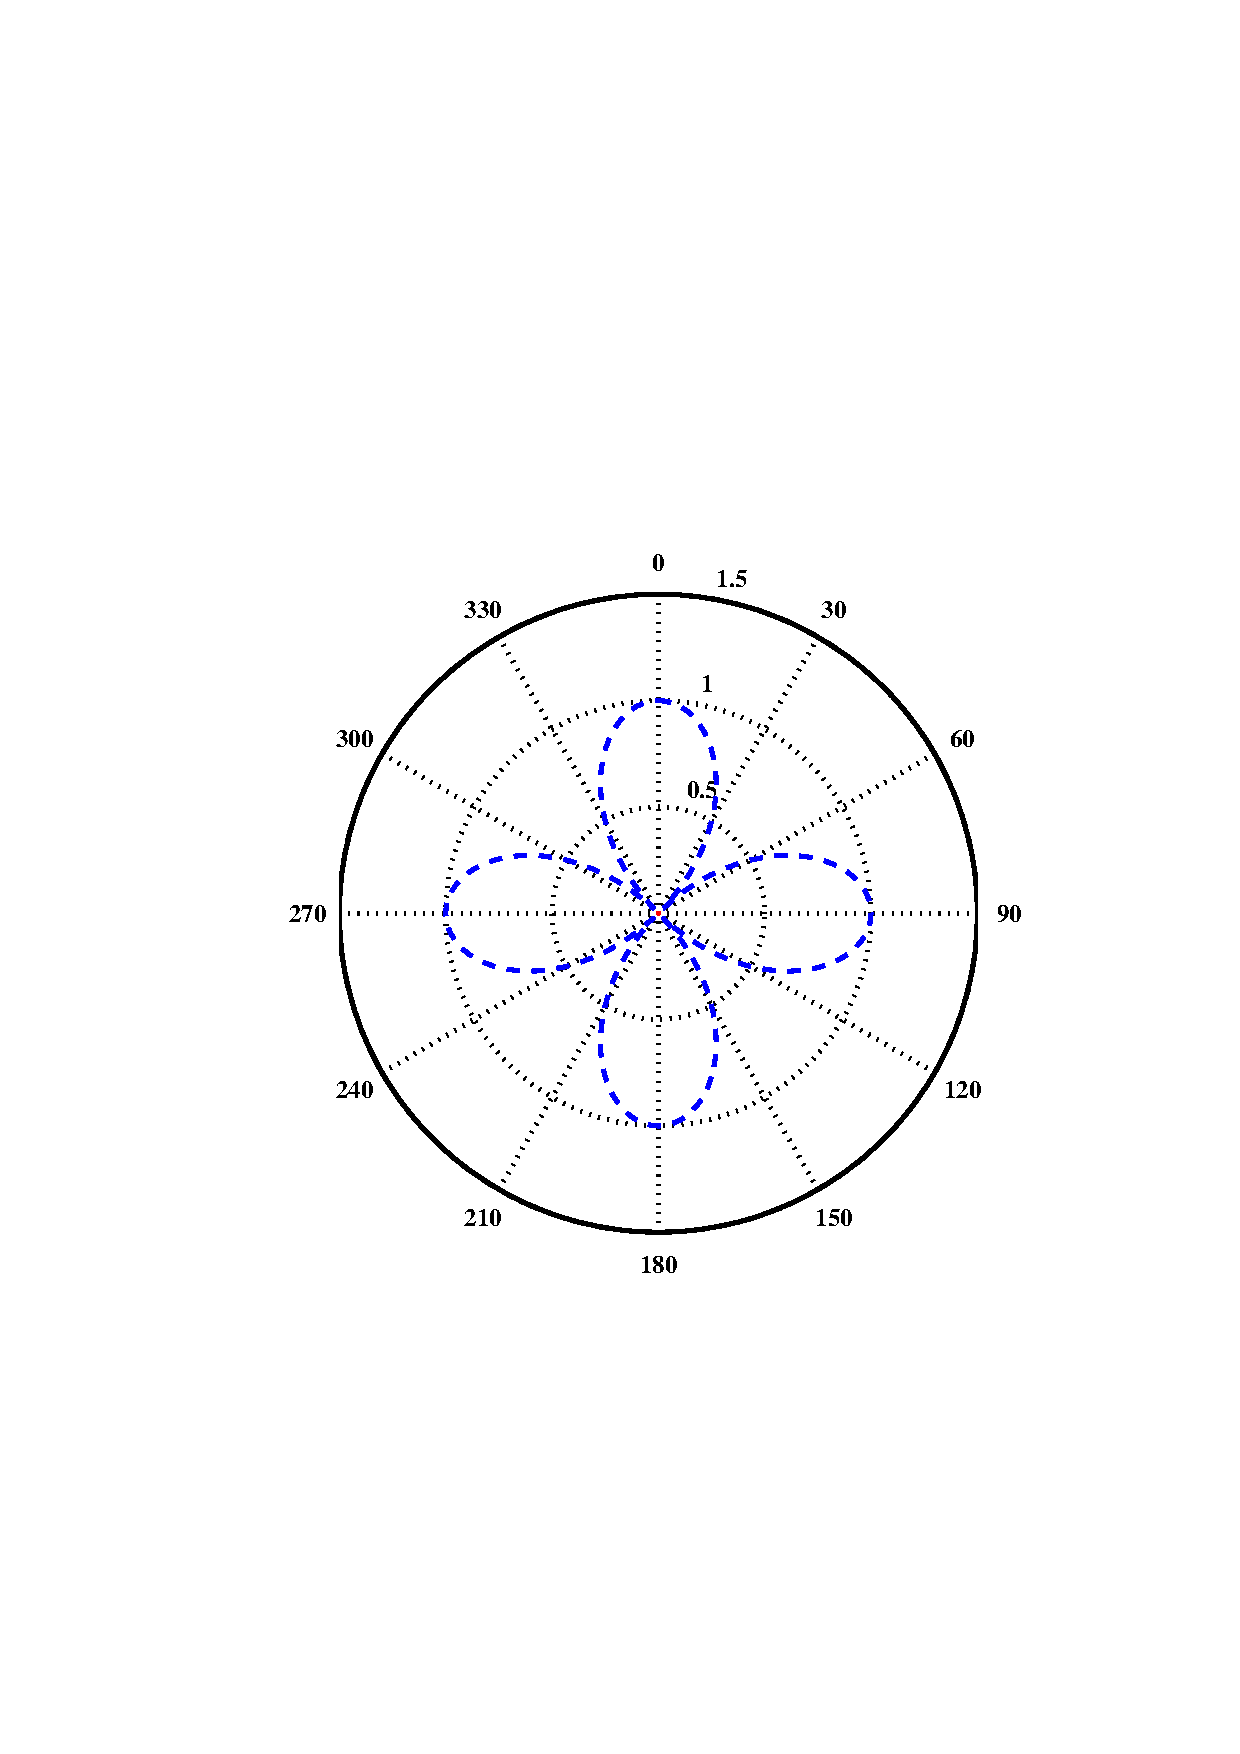
\includegraphics[width=5cm]{Figure/chapter02/radiationpattern/Fig/SS.pdf}}
        \caption{$V_p$(red)和$V_s$
			(blue)扰动的辐射模式。背景波场入射角为$0^{\circ}$,$360^{\circ}$接收不同模式的散射波场。
			 (a) PP, (b) PS, (c) SP和(d) SS模式.
    }
    \label{fig:radiationpattern} 
    \end{center}
\end{figure} 

\subsection{弹性波模式解耦}
弹性波场$\mathbf{u}=(u_x,u_y,u_z)$可以分解成P波波场与S波波场:$\mathbf{u}=\mathbf{u}^P+\mathbf{u}^S$,
其中,$\mathbf{u}^P=(u^P_x,u^P_y,u^P_z)$和$\mathbf{u}^S=(u^S_x,u^S_y,u^S_z)$.
对于各向同性介质而言,模式解耦是不依赖于模型参数的,可在波数域表示为(Zhang and McMechan, 2010)\cite[]{zhang.mcmechan:2010}:
\begin{equation}
        \tilde{\mathbf U}^P=\mathbf k(\mathbf k\cdot \tilde{\mathbf U}), \quad
        \tilde{\mathbf U}^S=-\mathbf 
        k\times(\mathbf k\times \tilde{\mathbf U})
\label{eq:Decomp}
\end{equation}
其中$\mathbf k=(k_x,k_y,k_z)$ 为归一化之后的波矢量,符号$\tilde{}$表示波数域波场。

根据前文推导, 将Fr{$\acute{e}$}chet导数分解为不同波模式:
\begin{equation}
        {\mathbf J}_M={\mathbf J}^P_M+{\mathbf J}^S_M,
\label{eq:PropaMDall}
\end{equation}
其中
\begin{equation}
        {\mathbf J}^P_M=\mathcal{F}^{-1}(\mathbf k(\mathbf k\cdot \tilde{\mathbf
        J}_M)), \quad
        {\mathbf J}^S_M=\mathcal{F}^{-1}(-\mathbf
                k\times(\mathbf k\times \tilde{\mathbf J}_M)),
\label{eq:PropaMDsplit}
\end{equation}
这里$\mathcal{F}^{-1}$表示从波数域到空间域的反Fourier变换,$\tilde{\mathbf{J}}_M$表示波数域的 Frech{$\acute{e}$}t导数。
这样,方程\eqref{eq:finalMatrixshort}可以按以下方式分裂成两部分:
\begin{equation}
        \mathbf{J}^P\delta\mathbf{m}=\mathbf{\delta u}^P,\quad
        \mathbf{J}^S\delta\mathbf{m}=\mathbf{\delta u}^S,
        \label{eq:UPandUS}
\end{equation}
其中
\begin{equation}
        \mathbf{\delta u}=\mathbf{\delta u}^P+\mathbf{\delta u}^S,
        \label{eq:UPS}
\end{equation}

\begin{equation}
        \mathbf{J}=\mathbf{J}^P+\mathbf{J}^S,
        \label{eq:JPS}
\end{equation}
这里$\mathbf{J}^P=(\mathbf{J}^P_{V_p}\quad\mathbf{J}^P_{V_s})$和$\mathbf{J}^S=(\mathbf{J}^S_{V_p}\quad\mathbf{J}^S_{V_s})$为大小是$K\times{2L}$的矩阵,分别代表P波或S波分量对应的Frech{$\acute{e}$}t导数(Jacobian矩阵)。
方程\eqref{eq:UPandUS}表示了在模式解耦下的Born近似所描述的散射波场。

我们知道,次级震源只有在背景波场入射到参数扰动的位置时才会被激发。尽管次级震源(或者说背景场)中会既有P波又有S波,
我们发现对于反演来说并不需要严格区分出它们的贡献(原因将在本章讨论部分进行详细阐述)。于是,模式解耦下Jacobian
矩阵满足:
\begin{equation}
        \begin{split} 
        \mathbf{J}^W_M(\mathbf{x}_l,\mathbf{r}_k)=
        \mathbf{T}_M(\mathbf{x}_l):\mathbf{G}'^W(\mathbf{x}_l,\mathbf{r}_k),\quad
        W\in\{P, S\}.
        \end{split}
        \label{eq:EquivFre1}
\end{equation}
该式说明模式解耦算子只作用在$\mathbf{G}'$上,即只作用在散射Green函数的空间导数上。虽然有些学者尝试用“解耦”的方式来
传播P和S波波场(马德堂和朱光明,2003\cite{马德堂2003}; Cheng et al.,
2016\cite{cheng:2016}),
但是只能在介质参数足够光滑的时候才能获得令人满意的结果(Brytik et al., 2011\cite{brytik:2011};
Wang and McMechan, 2015\cite{wang.mcmechan:2015b})。
因此,本文并未采用传播解耦波场的方法,而是用方程\eqref{eq:PropaMDsplit}来对演做的弹性总波场进行模式解耦。

\section{弹性波模式解耦全波形反演}
方程\eqref{eq:finalMatrixshort}对应的反问题是要找到一个能够解释地震数据的最优模型,它可以通过求解以下
目标函数的最小值问题来实现:
\begin{equation}
    E=\frac{1}{2}\delta\mathbf{d}^{\dagger}\delta\mathbf{d},
    \label{eq:misfit}
\end{equation}
其中$\delta\mathbf{d}$ 表示观测数据与模拟数据之间的残差向量,满足$\delta\mathbf{d}=\mathfrak{F}(\mathbf{u}_{obs}-\mathbf{u}_{cal})$,
这里$\mathfrak{F}$ 为位于接收点处的采样函数,上标$\dagger$表示共轭转置算子。求解该目标函数最小值的标准策略是
采用梯度类或者基于Hessian矩阵的最优化算法。可以通过Jacobian矩阵来求取梯度:
\begin{equation}
        \mathbf{g}=
        \begin{pmatrix}
                \mathbf{g}_{V_p}\\
                \mathbf{g}_{V_s}
        \end{pmatrix}
        =\mathfrak{R}\begin{pmatrix}
                \mathbf{J}^{\dagger}_{V_p}\delta \mathbf{d}\\
                \mathbf{J}^{\dagger}_{V_s}\delta \mathbf{d}
        \end{pmatrix},
        \label{eq:MatrixGra1}
\end{equation}
其中$\mathfrak{R}$表示取实部。为获得模型更新,梯度导引类方法利用$\mathbf{g}$,而Hessian类方法则利用了
梯度和Hessian矩阵的信息。Hessian类算法能保证二阶的收敛性,但即使是声波FWI也要付出庞大的计算与存储代价。
为了在效率与精度之间寻求平衡,通常会采用梯度类的方法迭代地求解方程\eqref{eq:misfit},即:
\begin{equation}
        \mathbf{m}_{k+1}=\mathbf{m}_{k}-\alpha_k \mathbf{g}_k,
        \label{eq:Gradientmethod1}
\end{equation}
其中$\mathbf{m}$是模型参数向量,$k$是迭代次数,$\alpha_k$和$\mathbf{g}_k$则分别是第$k$迭代的步长与梯度。
常规的EFWI需要非常多的迭代次数,因此良好的梯度预条件能够加速收敛。

方程\eqref{eq:MatrixGra1}中的梯度并没有内在的机制来判断数据残差中的成分是来自$\delta V_p$还是来自$\delta V_s$。
将方程\eqref{eq:MatrixGra1}分裂为P波与S波分量对应的两个部分:
\begin{equation}
        \begin{pmatrix}
                \mathbf{g}^P_{V_p}\\
                \mathbf{g}^P_{V_s}
        \end{pmatrix}
        =\mathfrak{R}\begin{pmatrix}
                [\mathbf{J}^P_{V_p}+\mathbf{J}^S_{V_p}]^{\dagger}\delta \mathbf{d}^P\\
                [\mathbf{J}^P_{V_s}+\mathbf{J}^S_{V_s}]^{\dagger}\delta \mathbf{d}^P
        \end{pmatrix},
        \label{eq:DEMatrixGraP}
\end{equation}
和
\begin{equation}
        \begin{pmatrix}
                \mathbf{g}^S_{V_p}\\
                \mathbf{g}^S_{V_s}
        \end{pmatrix}
        =\mathfrak{R}\begin{pmatrix}
                [\mathbf{J}^P_{V_p}+\mathbf{J}^S_{V_p}]^{\dagger}\delta \mathbf{d}^S\\
                [\mathbf{J}^P_{V_s}+\mathbf{J}^S_{V_s}]^{\dagger}\delta \mathbf{d}^S
        \end{pmatrix},
        \label{eq:DEMatrixGraS}
\end{equation}
其中,$\mathbf{g}^W_M$为特定波模式(W)的数据残差对应的某一物理参数(M)的梯度。
在对地面多分量地震记录进行P/S分离非常具有挑战,因此数据残差的的分解也会变得非常困难,尤其是在近地表介质不均匀且(或者)
边界条件不完整的情况下。因此需要采取策略来回避多分量地震记录的地面P/S分离。
\begin{figure}
    \begin{center}
        \includegraphics[width=1.0\textwidth]{Figure/chapter02/finalMarmousiII/Fig/zerolagLAST1.pdf}
        \caption{
			通过偏导数波场与数据残差之间的零延迟互相关计算梯度的示意图。为了简单说明,只在背景介质中放置单个的散射点。
%Schematic illustration of gradient calculation through zero-lag correlation
% between the partial derivative wavefields
%and the residual seismogram.
%Only a point perturbation is given in the background media for illustration.
    }
    \label{fig:crossterm}
    \end{center}
\end{figure}

目标函数的梯度可看作是偏导数波场与数据残差在时间域的零延迟互相关\cite[]{pratt1998gauss}。如图\ref{fig:crossterm}所示,
假设背景介质中有一个点扰动,数据残差为观测数据与模拟数据之间的差值。偏导数波场代表了由次级源产生的特征性点绕射响应。
一般而言,P波与S波背景速度不同,因而在偏导数波场和地震记录残差中它们的运动学特征(比如走时和曲率)也不同。
所以,相同波模式之间的零延迟互相关将在梯度计算中占主导,而不同波模式之间的互相关则会由于非同相的干涉叠加被基本消除掉。
因此,会有以下的交叉项近似:
\begin{equation}
        \begin{split}
                [\mathbf{J}_{V_p}^{S}]^{\dagger}\delta \mathbf{d}^P\approx\mathbf{0},\\
                [\mathbf{J}_{V_s}^{S}]^{\dagger}\delta \mathbf{d}^P\approx\mathbf{0},\\
                [\mathbf{J}_{V_p}^{P}]^{\dagger}\delta \mathbf{d}^S\approx\mathbf{0},\\
                [\mathbf{J}_{V_s}^{P}]^{\dagger}\delta \mathbf{d}^S\approx\mathbf{0},
        \end{split}
        \label{eq:crossterms}
\end{equation}
其中$\mathbf{0}$为空矩阵。
此外,散射模式说明P波速度的扰动不会产生S波散射,所以还有:
\begin{equation}
\mathbf{J}^S_{V_p}=\mathbf{0}.
\label{eq:Jsvp}
\end{equation}
从而得到:
\begin{equation}
        \begin{split}
[\mathbf{J}^S_{V_p}]^{\dagger}\delta \mathbf{d}^P=\mathbf{0}, \\
[\mathbf{J}^S_{V_p}]^{\dagger}\delta \mathbf{d}^S=\mathbf{0}.
        \end{split}
\label{eq:Jsvp1}
\end{equation}
\subsection{模式解耦梯度预条件}
利用方程\eqref{eq:crossterms}和\eqref{eq:Jsvp1},可以获得以下近似:
\begin{equation}
        \mathbf{J}^{\dagger}_{V_p}\delta \mathbf{d}^P\approx
        [\mathbf{J}^P_{V_p}]^{\dagger}\delta \mathbf{d},\quad
        \mathbf{J}^{\dagger}_{V_s}\delta \mathbf{d}^S\approx
        [\mathbf{J}^S_{V_s}]^{\dagger}\delta \mathbf{d}.
        \label{eq:crossterm}
\end{equation}
因此,基于模式解耦的梯度可以表示为:
\begin{equation}
        \begin{pmatrix}
                \mathbf{g}^P_{V_p}\\
                \mathbf{g}^P_{V_s}
        \end{pmatrix}
        \approx\mathfrak{R}\begin{pmatrix}
                [\mathbf{J}_{V_p}^{P}]^{\dagger}\delta \mathbf{d}\\
                [\mathbf{J}_{V_s}^{P}]^{\dagger}\delta \mathbf{d}
        \end{pmatrix},
        \label{eq:MatrixGraP}
\end{equation}
和
\begin{equation}
        \begin{pmatrix}
                \mathbf{g}^S_{V_p}\\ 
                \mathbf{g}^S_{V_s}
        \end{pmatrix}
        \approx\mathfrak{R}\begin{pmatrix}
                \mathbf{0}\\ 
                [\mathbf{J}^S_{V_s}]^{\dagger}\delta \mathbf{d}
        \end{pmatrix}.
        \label{eq:MatrixGraS}
\end{equation}
上述方程表明在梯度计算中可以通过Fr{$\acute{e}$}chet导数的解耦来代替数据残差的解耦。

进一步而言,由于串扰效应主要体现在P波数据中,因此本文提出舍弃梯度中的$\mathbf{g}_{V_s}^P$项来降低参数耦合效应。
于是,分别选取解耦后的P波与S波Fr{$\acute{e}$}chet导数来构建预条件之后$V_p$和$V_s$的梯度:
\begin{equation}
        \begin{pmatrix}
                \hat{\mathbf{g}}_{V_p}\\
                \hat{\mathbf{g}}_{V_s}
        \end{pmatrix}=
        \begin{pmatrix}
                \mathbf{g}_{V_p}^P\\
                \mathbf{g}_{V_s}^S
        \end{pmatrix}
        \approx 
        \mathfrak{R}\begin{pmatrix}
                [\mathbf{J}^P_{V_p}]^{\dagger} \delta \mathbf{d}\\
                [\mathbf{J}^S_{V_s}]^{\dagger} \delta \mathbf{d}
        \end{pmatrix}.
        \label{eq:MatrixGraMode}
\end{equation}
这里符号$\hat{}$指示基于模式解耦的预条件梯度。
最终,EFWI问题转化为通过模式解耦预条件共轭梯度(MDPCG)的方式来迭代求解:
\begin{equation}
        \mathbf{m}_{k+1}=\mathbf{m}_{k}-\alpha_k
        \begin{bmatrix}\mathbf{Q}_1\hat{\mathbf{g}}_{V_p}\\\mathbf{Q}_2\hat{\mathbf{g}}_{V_s}\end{bmatrix}_{k},
        \label{eq:Gradientmethod}
\end{equation}
其中,$\mathbf{Q}_1$和$\mathbf{Q}_2$表示进一步的预条件算子,比如采用能量照明对梯度进行补偿。步长$\alpha_k$采用抛物线拟合的方式来搜寻(Vigh
and Starr, 2008\cite[]{vigh20083d})。

\subsection{共轭状态法计算梯度}
显式地计算Fr{$\acute{e}$}chet导数需要进行多达模型网格数量的正演模拟次数,这在目前实际应用中无法实现\cite[]{virieux2009overview}。
为了避免显式构建Jacobian矩阵,文中采用共轭状态法来计算梯度\cite[]{tromp2005seismic,plessix2006}。利用Green函数的空间互易性,
方程\eqref{eq:MatrixGra1}中的原始梯度可以通过正传波场与反传的残差波场的时间域
零延迟互相关计算得到:
\begin{equation} 
        \begin{split}
        \mathbf{g}_{V_p}&=-2\rho V_p\int_{0}^{T}\frac{\partial u_i}{\partial
        x_j}\frac{\partial \psi_k}{\partial x_l}
        \delta_{ij}\delta_{kl}dt,\\
        \mathbf{g}_{V_s}&=-2\rho V_s\int_{0}^{T}\frac{\partial u_i}{\partial
        x_j}\frac{\partial \psi_k}{\partial x_l}
        (-2\delta_{ij}\delta_{kl}+\delta_{ik}\delta_{jl}+\delta_{il}\delta_{jk})dt,
        \end{split}
        \label{eq:Gradient_vpvs}
\end{equation}
其中$u_i$是从震源出发的正传波场,$\psi_k$ 为由数据残差从接收点处反传重建的共轭波场。注意方程\eqref{eq:Gradient_vpvs}
中第一行的算式中自动隐含了正传和共轭波场的散度算子。

从方程\eqref{eq:EquivFre1}可看出,Frech$\acute{e}$t导数的模式解耦等价于施加在散射Green函数上。这就意味着当使用伴随状态法时,
只需要解耦伴随波场就可以获得预条件后的梯度,即:
\begin{equation} 
        \begin{split} 
                \hat{\mathbf{g}}_{V_p}&=-2\rho V_p\int_{0}^{T}\frac{\partial u_i}{\partial
        x_j}\frac{\partial \psi^P_k}{\partial x_l}
        \delta_{ij}\delta_{kl}dt,\\
        &=-2\rho V_p\int_{0}^{T}\frac{\partial u_i}{\partial
        x_j}\frac{\partial \psi_k}{\partial x_l}
        \delta_{ij}\delta_{kl}dt,\\
                \hat{\mathbf{g}}_{V_s}&=-2\rho V_s\int_{0}^{T}\frac{\partial u_i}{\partial
        x_j}\frac{\partial \psi^S_k}{\partial x_l}
        (\delta_{ik}\delta_{jl}+\delta_{il}\delta_{jk})dt,
        \end{split}
        \label{eq:DeGradient_vpvs} 
\end{equation}
其中$\psi^P$和$\psi^S$分别为P波和S波的伴随波场。由于$\mathbf{g}_{V_p}$的计算中隐含了散度算子,总是满足$\hat{\mathbf{g}}_{V_p}=\mathbf{g}_{V_p}$。
与方程\eqref{eq:Gradient_vpvs}对比,由于S波的散度总是为0,所以在计算预条件后的S波速度梯度时舍弃了$-2\delta_{ij}\delta_{kl}$项。
因此,对于P波速度而言,模式解耦已经自动隐含在梯度计算中,但是对S波速度梯度的模式解耦预条件需要显式地施加。

解耦伴随波场需要额外的计算量,主要体现在每个时间片中需要两次Fourier变换。为了减少计算量并节省内存消耗,可以
对正传波场与反传波场在时间轴上进行重采样,并且在互相关之前只对反传的伴随波场进行模式解耦。
当其它多尺度策略考虑进来的时候,也可以对正传波场进行解耦,例如在某一阶段反演中单独使用SS或者PS模式。但本文并不推荐
这样的策略,这将在讨论部分进行阐述。
\section{模式解耦降低参数耦合的理论机制}
	前一节提出了通过模式解耦来预条件处理EFWI的梯度,以便压制参数耦合效应。然而解决参数解耦问题最直接有效(但也最昂贵)
的方法是考虑Hessian矩阵的优化方法。下面将采用解耦后的
Frech$\acute{e}$t导数来调查Hessian和分辨率矩阵的性质,并且对比GN,PCG与MDPCG方法的梯度来
阐明模式解耦EFWI能压制参数耦合的内在机制。
\subsection{Hessian矩阵及其不同模式的分量}
多参数情况下的Hessian矩阵是一个具有块状结构的对称方阵,其中非对角块测量了不同物理参数的偏导数波场之间的互相关效应,其作用
是消除多参数反演中的参数耦合效应。当反问题为近似线性或者数据残差非常小的时候,全Hessian将约等于近似Hessian
\cite[]{pratt1998gauss}:
\begin{equation}
\mathbf{H}_a =\mathfrak{R}[{\mathbf{J}}^{\dagger}\mathbf{J}]. 
\label{eq:hess}
\end{equation}
考虑到Fr{$\acute{e}$}chet导数的解耦(见方程\ref{eq:JPS}),可以将 $\mathbf{H}_a$ 分解为四个分量:
\begin{equation}
\begin{split}
\mathbf{H}_a^{PP}=\mathfrak{R}[{\mathbf{J}^{P}}]^{\dagger}[{\mathbf{J}^{P}}],\\
\mathbf{H}_a^{PS}=\mathfrak{R}[{\mathbf{J}^{P}}]^{\dagger}[{\mathbf{J}^{S}}],\\
\mathbf{H}_a^{SP}=\mathfrak{R}[{\mathbf{J}^{S}}]^{\dagger}[{\mathbf{J}^{P}}],\\
\mathbf{H}_a^{SS}=\mathfrak{R}[{\mathbf{J}^{S}}]^{\dagger}[{\mathbf{J}^{S}}].
\end{split}
\label{eq:hessian_component}
\end{equation}

\begin{figure}[!htb]
    \begin{center}
        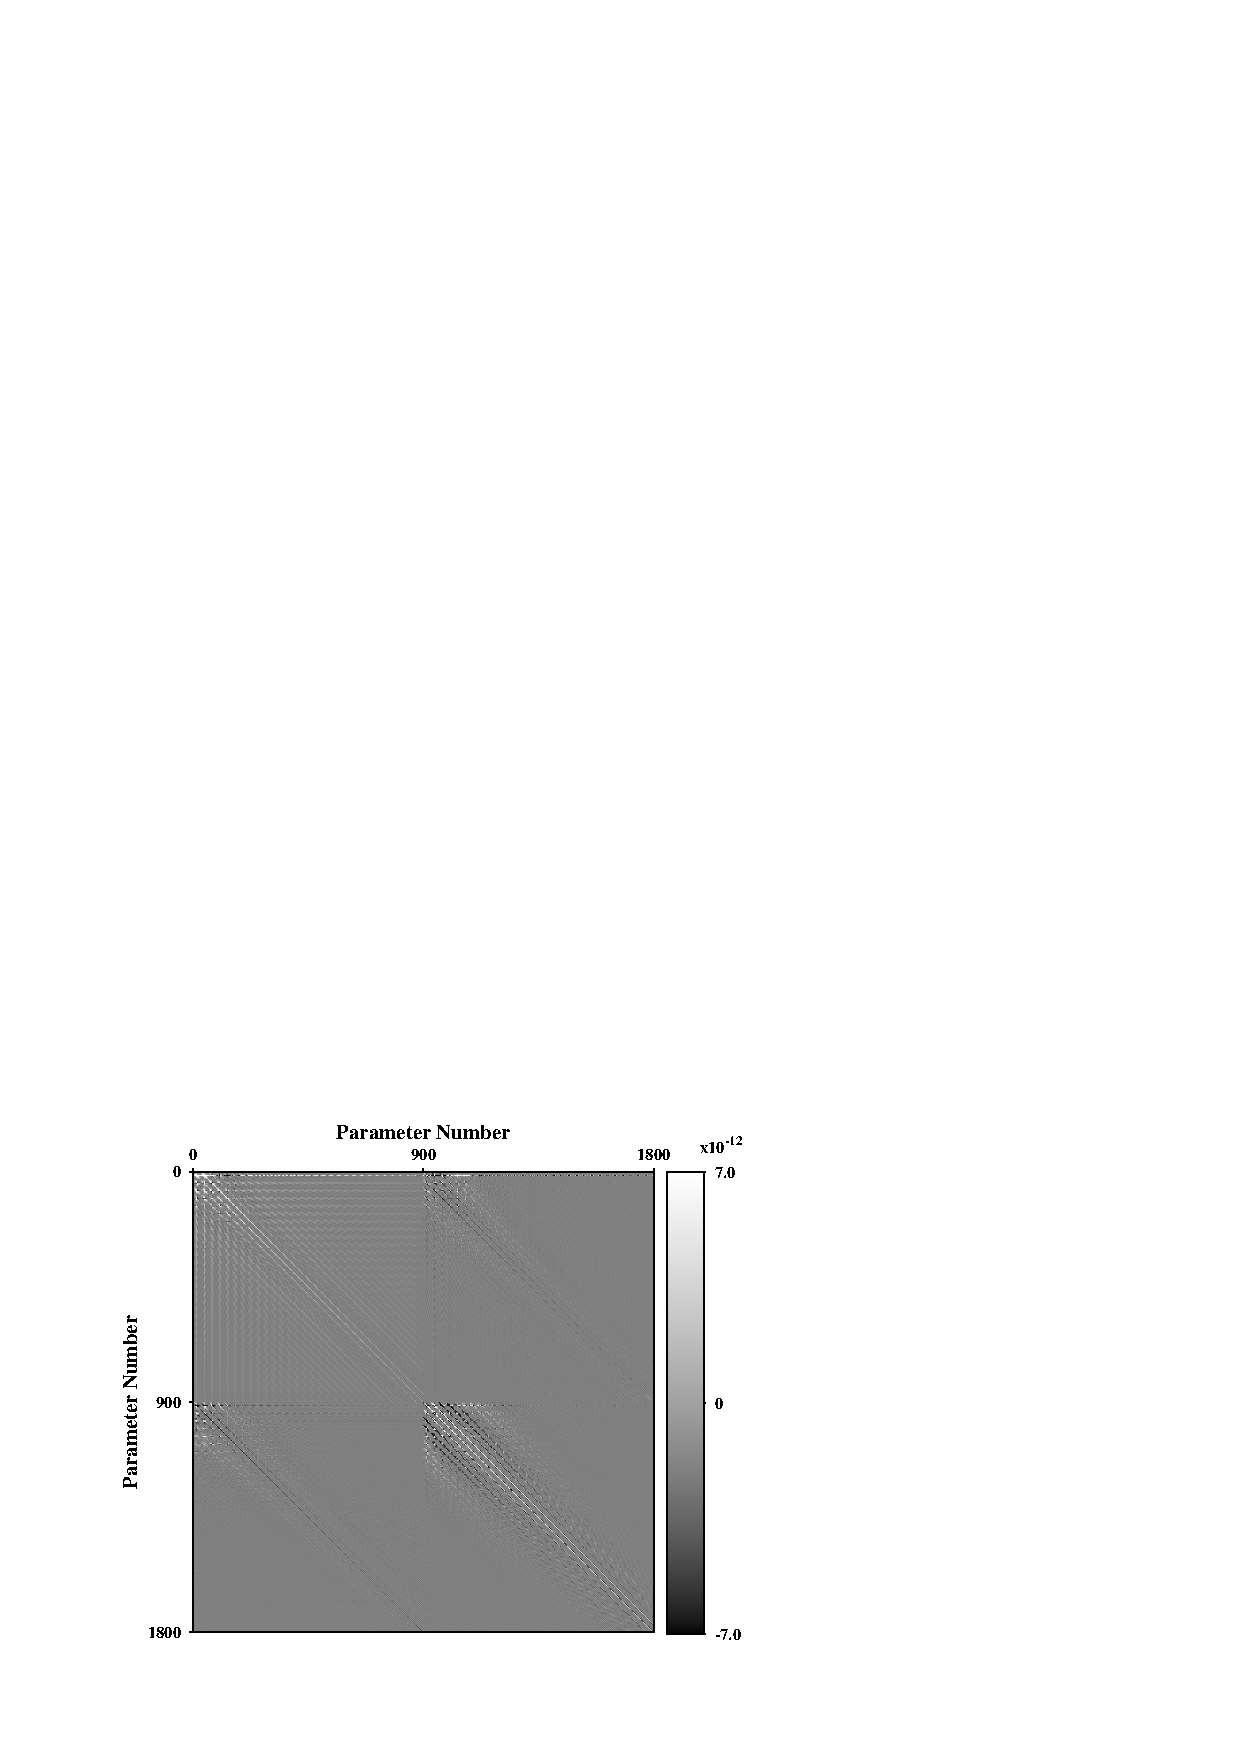
\includegraphics[width=10cm]{Figure/chapter02/ResoOpera/Fig/hessian.pdf}
        \caption{
            近似Hessian矩阵$\mathbf{H}_a$.
    }
    \label{fig:Hessian} 
    \end{center}
\end{figure}
\begin{figure}[!htb]
    \begin{center}
        \includegraphics[width=12cm]{Figure/chapter02/ResoOpera/Fig/fourhessian.pdf}
        \caption{
            近似Hessian矩阵的四个分量:
                        (a) $\mathbf{H}_a^{PP}$,
            (b) $\mathbf{H}_a^{PS}$, (c) $\mathbf{H}_a^{SP}$ and (d)$\mathbf{H}_a^{SS}$.
    }
    \label{fig:fourHessian}
    \end{center}
\end{figure}
从大规模应用问题来讲,Hessian矩阵通常是无法计算的。为了调查每个分量各自的贡献,这里在一个网格大小为$30\times30$,
空间采样为5m的模型上数值地计算出Hessian矩阵的各个分量。在模型的顶部中央放置一个纯P波震源,接收点分布于四个边界上。
近似Hessian矩阵(图\ref{fig:Hessian})及其分量(图\ref{fig:fourHessian})通过时间域的
Frech{$\acute{e}$}t导数显式
计算。近似Hessian矩阵中非对角块中明显的非零元素代表了很强的参数耦合效应。可以观察到以下
现象:
首先,交叉项分量,$\mathbf{H}_a^{PS}$和$\mathbf{H}_a^{SP}$对$\mathbf{H}_a$的贡献可以忽略不计。这是由于
背景P波和S波速度不同导致
相应
的P波与S波Fr{$\acute{e}$}chet导数
不具有相干性。
注意到,在这些交叉项分量中会有一些非常小值的非零元素。
这是由于Fr{$\acute{e}$}chet导数中震源附近的异常值所导致的。故有:
\begin{equation}
        \mathbf{H}_a\approx
        \mathbf{H}_a^{PP}+
        \mathbf{H}_a^{SS}.
        \label{eq:C3}
\end{equation}
其次,$\mathbf{H}_a$的非对角区块几乎与$\mathbf{H}_a^{PP}$一样,并且$\mathbf{H}_a^{SS}$只在右下对角快是非零的,
这是因为$\mathbf{J}^S=(\mathbf{0}\quad\mathbf{J}^S_{V_s})$。这些现象进一步确认了参数耦合主要是来自P波波场而非S波波场。
\subsection{模型分辨率矩阵及其分量}
通过模式解耦的Frech{$\acute{e}$}t导数对Hessian矩阵的定性分析并不足以理解解耦对反演产生作用的机制。为了评估P波与S波数据对
反演的贡献,我们进一步分析模式解耦如何在模型空间影响分辨率矩阵。模型的分辨率矩阵通常采用Hessian矩阵及其逆矩阵来计算得到
(Menke, 1989\cite[]{menke:1989}; Snieder and Trampert, 1999\cite{snieder1999inverse})。就方程\eqref{eq:finalMatrixshort}对应的反问题,采用以下公式来更新模型:
\begin{equation}
	\delta \tilde{\mathbf{m}}=-\mathbf{H}^{-1}_a\mathbf{J}^{\dagger}\delta 
        \mathbf{d},
        \label{eq:LeastSol}
\end{equation}
其中$\delta\tilde{\mathbf{m}}$为用全部数据残差估计得到的模型扰动。根据Born近似$\delta\mathbf{d}=\mathfrak{F}{\delta\mathbf{u}}$,
将方程\eqref{eq:finalMatrixshort}带入到式\eqref{eq:LeastSol}中,并省略采样函数$\mathfrak{F}$,可得:
\begin{equation}
	\delta \tilde{\mathbf{m}}=\mathbf{R}\delta \mathbf{m},
	\label{eq:ResoMatr}
\end{equation}
其中$\delta \mathbf{m}$表示真实模型扰动,且模型分辨率矩阵$\mathbf{R}$满足:
\begin{equation}
        \mathbf{R}=-\mathbf{H}^{-g}_a\mathbf{H}_a. 
        \label{eq:ResoOper} 
\end{equation}
注意,由于有限的观测导致近似Hessian总是病态的,因此这里采用Hessian的伪逆(广义逆)$\mathbf{H}^{-g}_a$,而不是真实的逆$\mathbf{H}^{-1}_a$。

\begin{figure*}
    \begin{center}
        \includegraphics[width=10cm]{Figure/chapter02/ResoOpera/Fig/resolutionmatrix.pdf}
        \caption{
			分辨率矩阵示意图。对于双参数的反问题,分辨率矩阵可以分成四个区块。
    }
    \label{fig:IllustrReso}
    \end{center}
\end{figure*}
如图\ref{fig:IllustrReso}所示,模型分辨率矩阵可看作是作用在真实模型上的滤波器。如果观测手段足够好,则分辨率矩阵会是严格的单位矩阵,
即$\mathbf{R}=\mathbf{I}$,那么模型参数也会是唯一确定的。然而,通常情况下$\mathbf{R} \ne \mathbf{I}$,因此对模型的估计将是真实模型参数的加权平均值。
$\mathbf{R}$ 的对角区块隐含了单参数内部间的相互影响及其相应的分辨能力,而非对角区块则反映了不同参数之间的相互影响。如果对角区块上有明显的非零元素分布,
则预示着不可忽视的参数耦合效应。若采用分解后的P波数据,则方程\eqref{eq:LeastSol} 变为:
\begin{equation}
        \delta \tilde{\mathbf{m}}^P=-\mathbf{H}^{-1}_a\mathbf{J}^{\dagger}\delta \mathbf{d}^P,
        \label{eq:LeastSolP}
\end{equation}
其中$\delta \tilde{\mathbf{m}}^P$ 表示P波数据给出的模型估计。同样采用式\eqref{eq:LeastSol}至式\eqref{eq:ResoOper}的推导,
可得P波数据的模型分辨率矩阵:
\begin{equation}
        \mathbf{R}^P=-\mathbf{H}^{-g}_a\mathbf{H}_a^P,
        \label{eq:ResoOperP}
\end{equation}
其中$\mathbf{H}_a^P=\mathbf{J}^{\dagger}\mathbf{J}^P$。类似的,S波的分辨率矩阵为:
\begin{equation}
        \mathbf{R}^S=-\mathbf{H}^{-g}_a\mathbf{H}_a^S,
        \label{eq:ResoOperS}
\end{equation}
且$\mathbf{H}_a^S=\mathbf{J}^{\dagger}\mathbf{J}^S$。容易证明$\mathbf{R}=\mathbf{R}^P+\mathbf{R}^S$。

\begin{figure}[!htb]
    \begin{center}
        \includegraphics[width=8cm]{Figure/chapter02/ResoOpera/Fig/resolutionoriginal.pdf}
        \caption{
分辨率矩阵及其不同波模式的分量
%Resolution matrix and its components:
(a) $\mathbf{R}$, (b) $\mathbf{R}^P$ and (c) $\mathbf{R}^S$.
    }
    \label{fig:Resolution}
    \end{center}
\end{figure}
同样采用前文小模型,可以显式计算出模型分辨率矩阵$\mathbf{R}$,$\mathbf{R}^P$和$\mathbf{R}^S$。
原始分辨率矩阵(图\ref{fig:Resolution}a)为带状对角阵,对角元素为小于1的正值。这说明了近似Hessian的逆可以为$V_p$和$V_s$的反演
提供很好的预条件。P波与S波数据对应的分辨率矩阵(图\ref{fig:Resolution}b和c)展示了一些有趣的现象。例如,$\mathbf{R}^P$和$\mathbf{R}^S$的对角块
构成了$\mathbf{R}$。除了一些由于震源附近的干扰而导致的假象,$\mathbf{R}^P$的底部两个区块都为空矩阵。在$\mathbf{R}^P$和$\mathbf{R}^S$的右上区块,它们的元素值
大小相等符号相反,两者相加为零从而能够使得$\mathbf{R}$右上区块为空。这些特征说明,对与线性的反问题(无cycle-skipping),P波与S波都对反演$V_p$有贡献,
而P波对$V_s$的贡献非常弱。常规的梯度法由于只用P波数据来计算$V_p$梯度(见式\ref{eq:Gradient_vpvs}),而这部分P波数据有可能来自$V_s$扰动,从而导致反演受到
参数耦合的影响。此外,单独用S波数据可以很好的分辨$V_s$。模式解耦的预条件方式正好利用了上述特征,因而其能够压制反演中参数间的耦合。
\subsection{与Gauss-Newton梯度的比较}
GN方法利用近似Hessian的逆对梯度进行预条件来处理参数之间的耦合效应:
\begin{equation}
\delta\tilde{\mathbf{m}} = - \mathbf{H}^{-1}_a\mathbf{g}.
\label{eq:GN}
\end{equation}
假设$\mathbf{H}_a$的伪逆为:
\begin{equation}
        \mathbf{H}^{-g}_a=    
        \begin{bmatrix}
                \mathbf{D}&\mathbf{E} \\
                \mathbf{F}&\mathbf{G}
        \end{bmatrix},
        \label{eq:HessInv}
\end{equation}
则GN方法实际上利用以下公式来更新模型:
\begin{equation}
    \mathbf{{m}}_{k+1}
    =\mathbf{{m}}_{k}-\alpha_k 
    \begin{bmatrix}
        \mathbf{D}\mathbf{g}^P_{V_p} +
        \mathbf{E}\mathbf{g}^P_{V_s}+
        \mathbf{E}\mathbf{g}^S_{V_s}\\
        \mathbf{G}\mathbf{g}^S_{V_s}
    \end{bmatrix}_{k},
    \label{eq:PreGNFi}
\end{equation}
因为
\begin{equation}
        \delta \mathbf{V}^P_s\approx0, \quad \delta \mathbf{V}_s \approx \delta
        \mathbf{V}^S_s=-\mathbf{G}\mathbf{g}^S_{V_s},
        \label{eq:KeyPoint}
\end{equation}
(见附录A)。
\begin{figure}[!htb]
    \begin{center}
        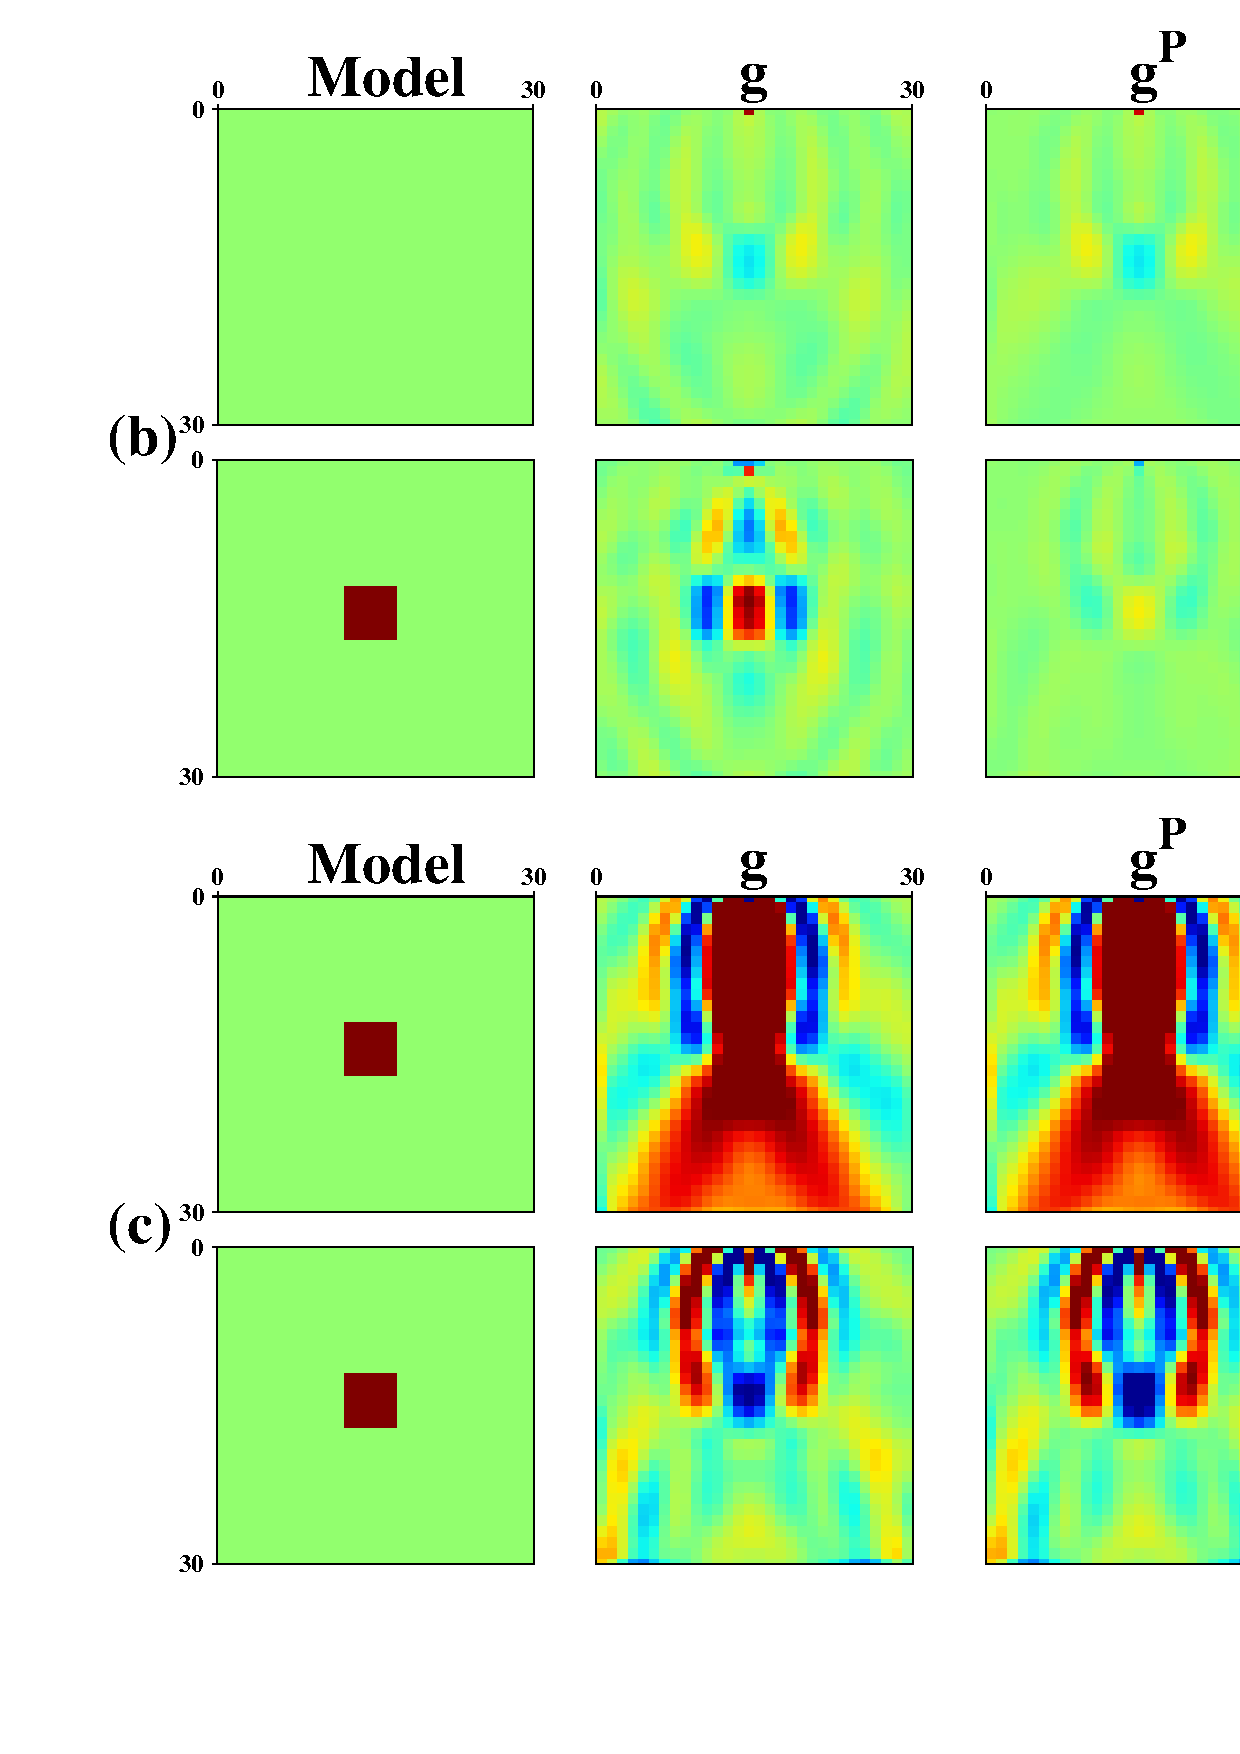
\includegraphics[width=14cm]{Figure/chapter02/Hessiantest/Fig/newepsall.pdf}
        \caption{
			PCG、GN以及MDPCG方法的第一次迭代梯度之间的对比。
    (a) $\delta V_p \neq 0$, $\delta V_s=0$; (b) $\delta V_p=0$, $\delta V_s\neq0$; and (c)
    $\delta V_p=10 \delta V_s$.
	从上到下为三个面板,每个面板中包含2行7列。第一行对应$V_p$,
	第二行对应$V_s$。7列从左到右依次为真实模型$\mathbf{m}=(\mathbf{V}_p,
    \mathbf{V}_s)$;
    PCG梯度$\mathbf{g}=(\mathbf{g}_{V_p},\mathbf{g}_{V_s})$,
    $\mathbf{g}^P=(\mathbf{g}^P_{V_p},\mathbf{g}^P_{V_s})$,
    $\mathbf{g^S}=(\mathbf{g}^S_{V_p},\mathbf{g}^S_{V_s})$;
    GN 梯度$\delta
    \tilde{\mathbf{m}}=(\delta\tilde{\mathbf{V}}_p,\delta\tilde{\mathbf{V}}_s)$;
        MDPCG梯度$\delta
        \tilde{\mathbf{m}}^P=(\delta\tilde{\mathbf{V}}^P_p,\delta\tilde{\mathbf{V}}^P_s)$
         $\delta
        \tilde{\mathbf{m}}^S=(\delta\tilde{\mathbf{V}}^S_p,\delta\tilde{\mathbf{V}}^S_s)$。
    }
    \label{fig:all}
    \end{center}
\end{figure}

在图\ref{fig:all}中,我们同样采用前文小模型实验来比较PCG、GN和MDPCG方法的梯度。
在模型中央放置三种不同类型、尺度为10$\times$10m的参数扰动组合,分别为:(a) $\delta V_p \neq 0$, $\delta V_s = 0$; (b) $\delta V_p = 0$,
$\delta V_s \neq 0$,和(c) $\delta V_p =10\delta
V_s$。初始模型为均匀的背景速度。在第一组实验中只有P波数据,可以看到原始的梯度($\mathbf{g}_{V_p}$和$\mathbf{g}_{V_s}$)中,有非常明显的参数耦合效应。
从图\ref{fig:all}a和b中可以看到,对于物理参数A而言,另一个参数B扰动会产生一个与B扰动方向相反的A的梯度。从图\ref{fig:all}b和c中$\mathbf{g}^{P}_{V_s}$看到,尽管P波数据残差可能携带了$\delta V_s$的信息,
常规梯度类方法用P波数据来反演$V_s$将会受到参数耦合的影响。在第三组实验中,由于参数耦合的影响,$\mathbf{g}^P_{V_s}$甚至提供了错误的更新方向。
由于S波残差只与$\delta
V_s$有关,因此正如我们所期望,$\mathbf{g}^S_{V_s}$总是能提供一个正确的更新方向。所以,$\mathbf{g}^P_{V_s}$是梯度中参数耦合部分的主导者。
一般来说,在以P波能量占主导的地震数据中,梯度中的这种耦合成分总是带来负面的影响,除非采用行之有效的预条件算子,例如图\ref{fig:all}中的GN梯度。

更重要的是,图\ref{fig:all}中最后三列在数值上验证了方程\eqref{eq:KeyPoint},同时也展示了模式解耦梯度法与GN方法之间的异同。与常规梯度法不同,
GN方法利用Hessian的逆以不同权重叠加三个解耦之后的梯度
($\mathbf{g}^P_{V_p}$、$\mathbf{g}^P_{V_s}$和$\mathbf{g}^S_{V_s}$),来实现P波速度梯度的最佳预条件。对于S波速度,GN方法实际上用
$\mathbf{G}$做为算子来对S波速度梯度($\mathbf{g}^S_{V_s}$)做预条件处理。算子$\mathbf{G}$近似等价于$[\mathbf{J}^{S}_{V_s}]^{\dagger}\mathbf{J}^{S}_{V_s}$的伪逆
(见方程\ref{eq:ResoOperS2})。正如方程\eqref{eq:Gradientmethod}所示,模式解耦梯度法也需要进一步的预条件来加速收敛。例如,预条件算子$\mathbf{Q}_2$
只需要考虑S波的照明补偿以及子波带宽效应即可,即近似$\mathbf{G}$的效果。因此,对
$V_s$反演,模式解耦梯度法几乎可看作是采用解耦的S波数据进行的单参数反演。相应地,预条件算子$\mathbf{Q}_2$要更廉价一些,比如利用单参数拟Hessian或者l-BFGS
方法。这种预条件方法为$V_s$反演近似提供了GN梯度同时又降低了迭代中的参数耦合,能够在不引入Hessian的情况下加速收敛。

\section{数值实验}
本节用两个理论合成数据的例子来验证模式解耦EFWI的有效性。实验中我们采用纯P波震源来合成多分量地震记录。
从较好的初始模型开始,$V_p$和$V_s$将同时被反演。在时间域对数据进行低通滤波,然后采用从低频到高频的多尺度策略来避免陷入局部极值。反演
分为四个不同的阶段:0-2Hz,0-4Hz,0-6Hz和0-10Hz。整个数值实验中,采用原始梯度的PCG与采用模式解耦梯度的MDPCG法都使用了随深度变化的照明补偿算子来进行预条件\cite[]{kohn:2012}。
\subsection{流体饱和模型}
图\ref{fig:smallmodel}定义了一个在砂岩背景模型中的流体饱和储层,背景模型参数为$V_p=3.14 km/s$, $V_s=1.56 km/s$以及$\rho=2000 kg/m^{-3}$。储层的上部含气饱和,参数为
$V_p=2.6 km/s$和$V_s=1.66 km/s$,下部含水,$V_p=3.0 km/s$和$V_s=1.66 km/s$。
储层的速度值根据砂岩岩石物理模型给出\cite[]{mavko2009rock}。在模型顶部放置炮点和检波器,合成32炮数据,炮间距为100m,每炮数据为400道记录,道间距为10m。反演以背景模型作为初始模型。
每阶段最大迭代次数限制为10次。从反演结果上看,常规EFWI方法能得到可接受的$V_p$模型,而$V_s$反演结果受参数耦合影响则非常糟糕。
这是因为在初始阶段,梯度会受到参数耦合的强烈影响,导致模型中长波长成分的重建受到严重干扰,因此在有限的迭代次数下反演最终收敛到了局部极值。
采用了模式解耦梯度的MDPCG之后,EFWI最后很好的重建了$V_p$和$V_s$模型。
\begin{figure}[!htb]
    \begin{center}
		\subfloat[]{\includegraphics[width=5cm]{Figure/chapter02/smallmodel/Fig/truevp.pdf}}
		\subfloat[]{\includegraphics[width=5cm]{Figure/chapter02/smallmodel/Fig/truevs.pdf}}\\
		\subfloat[]{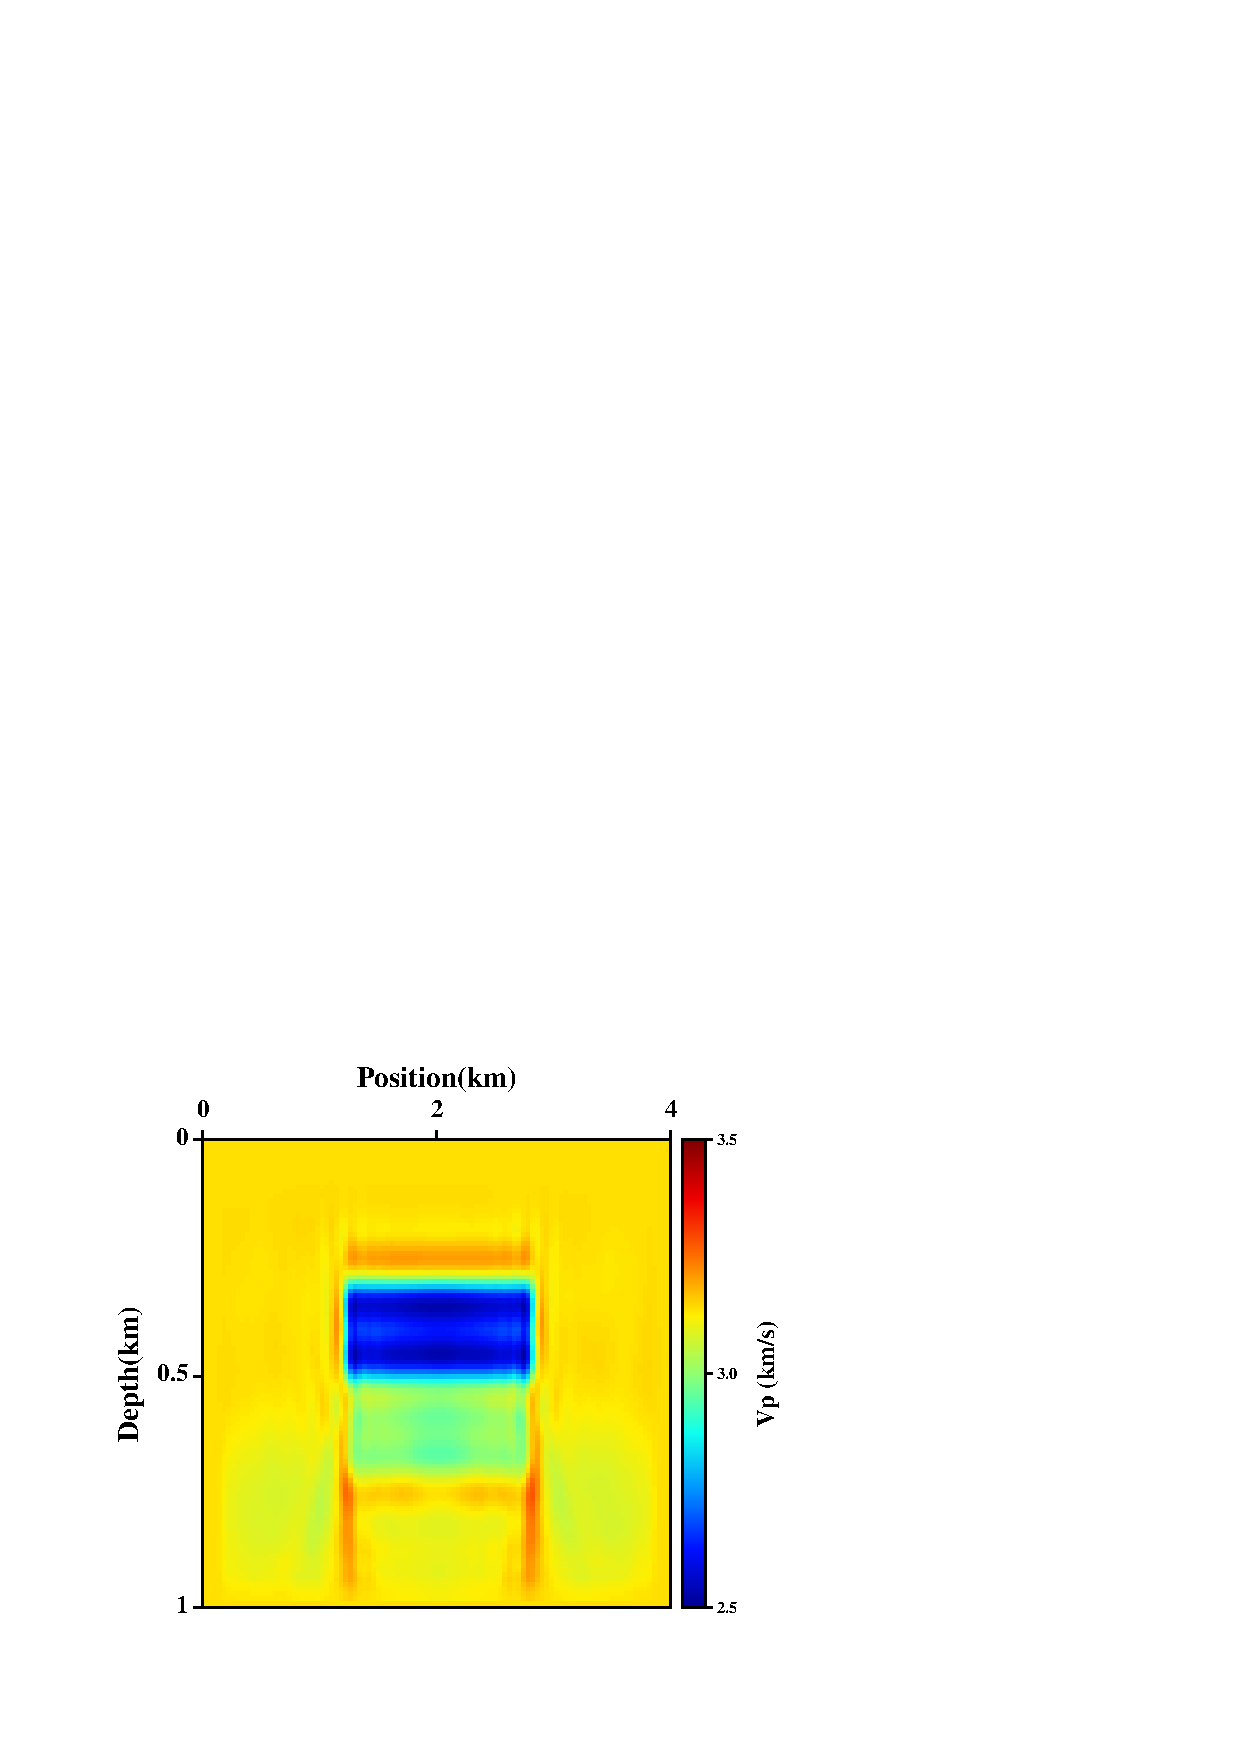
\includegraphics[width=5cm]{Figure/chapter02/smallmodel/Fig/nodecomvp.pdf}}
		\subfloat[]{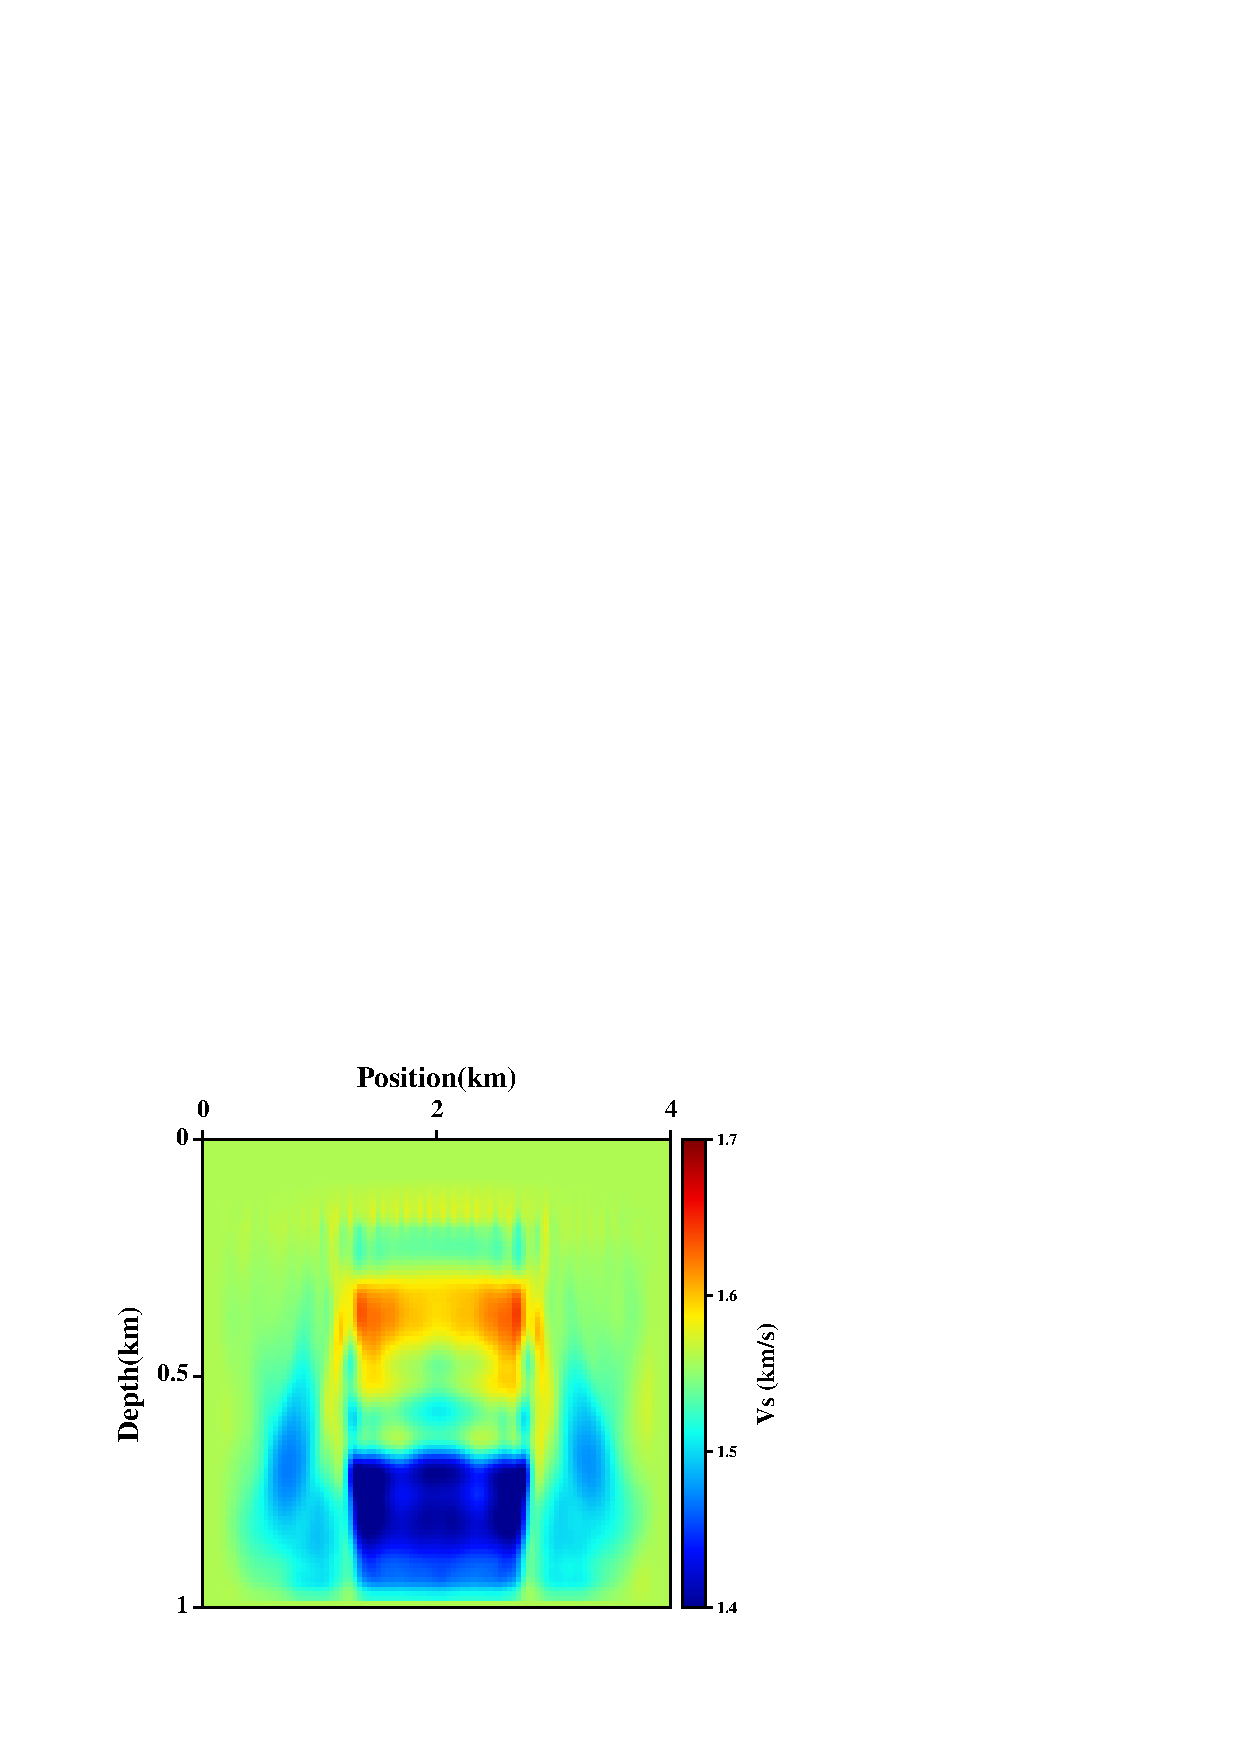
\includegraphics[width=5cm]{Figure/chapter02/smallmodel/Fig/nodecomvs.pdf}}\\
		\subfloat[]{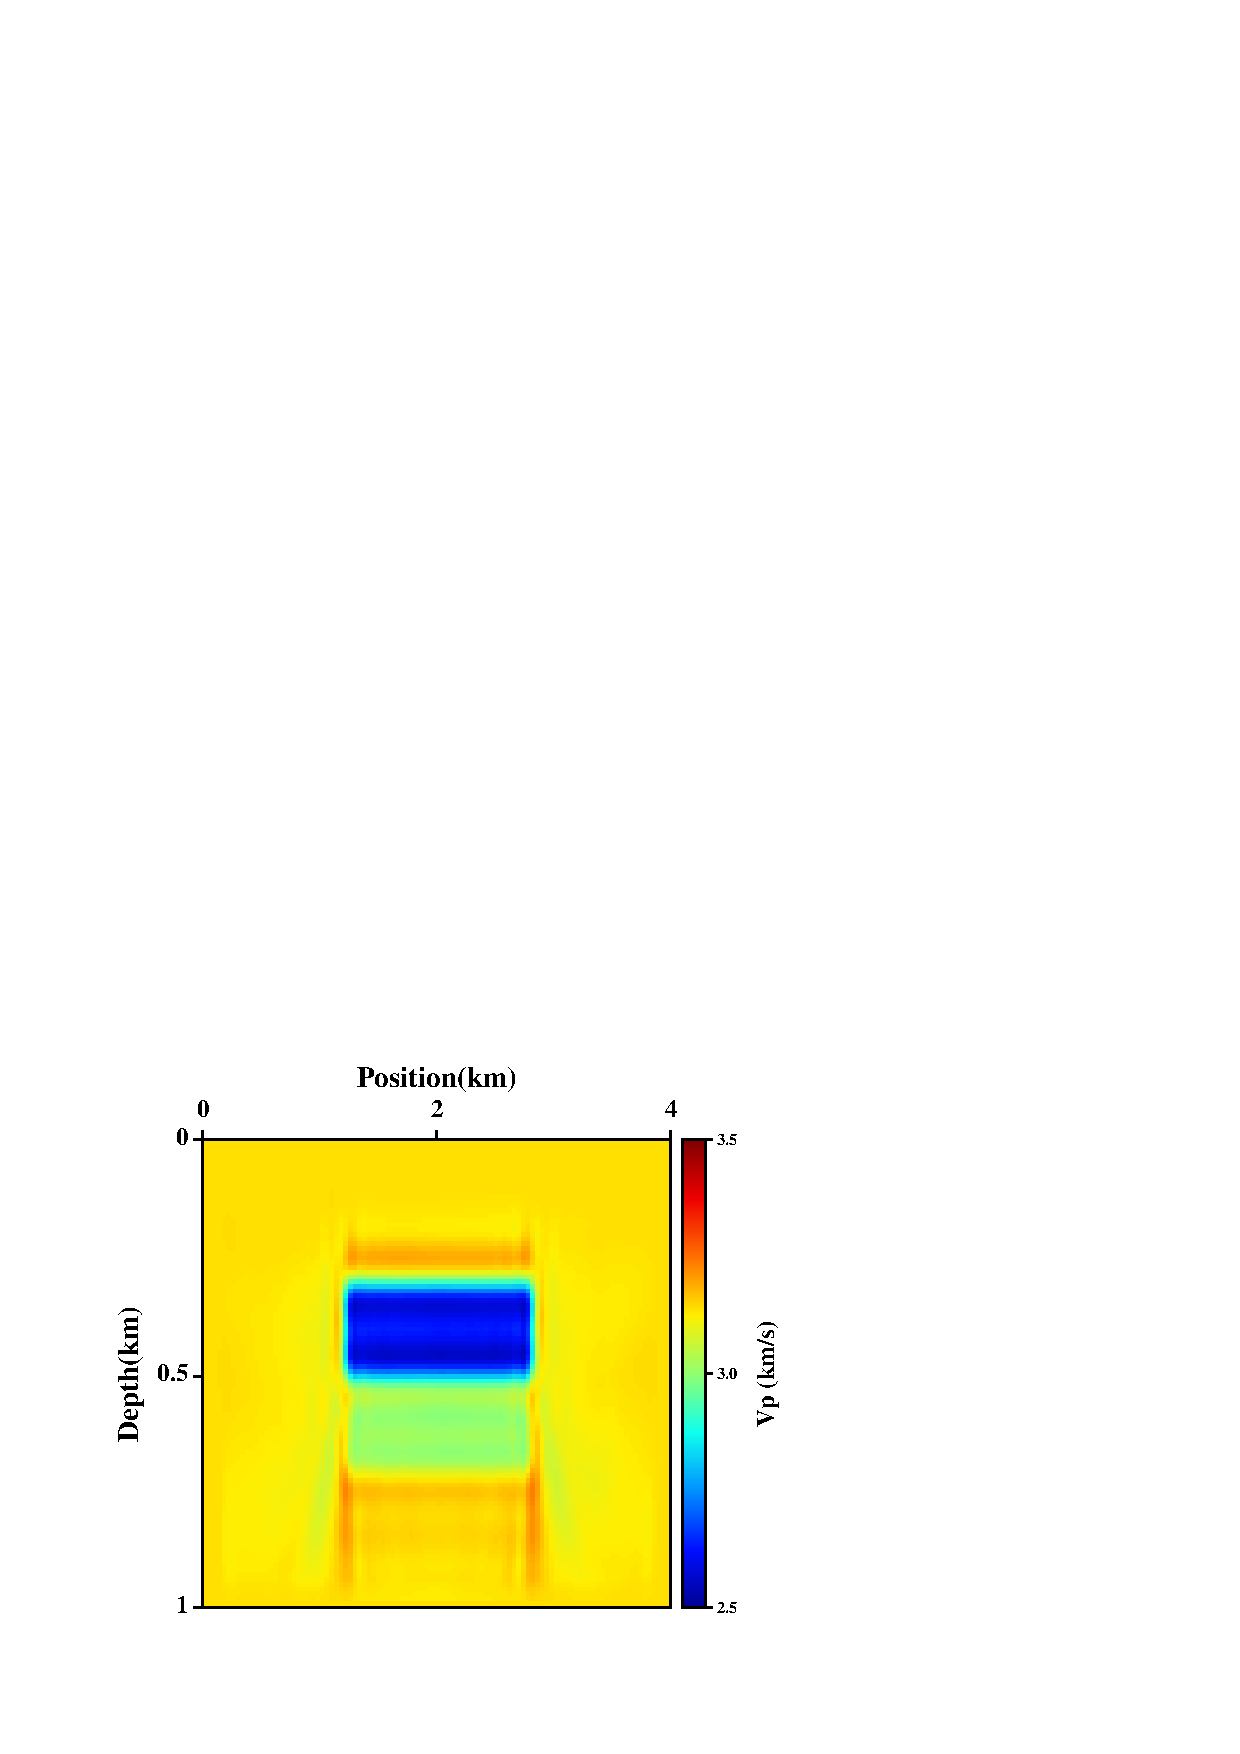
\includegraphics[width=5cm]{Figure/chapter02/smallmodel/Fig/decomvp.pdf}}
		\subfloat[]{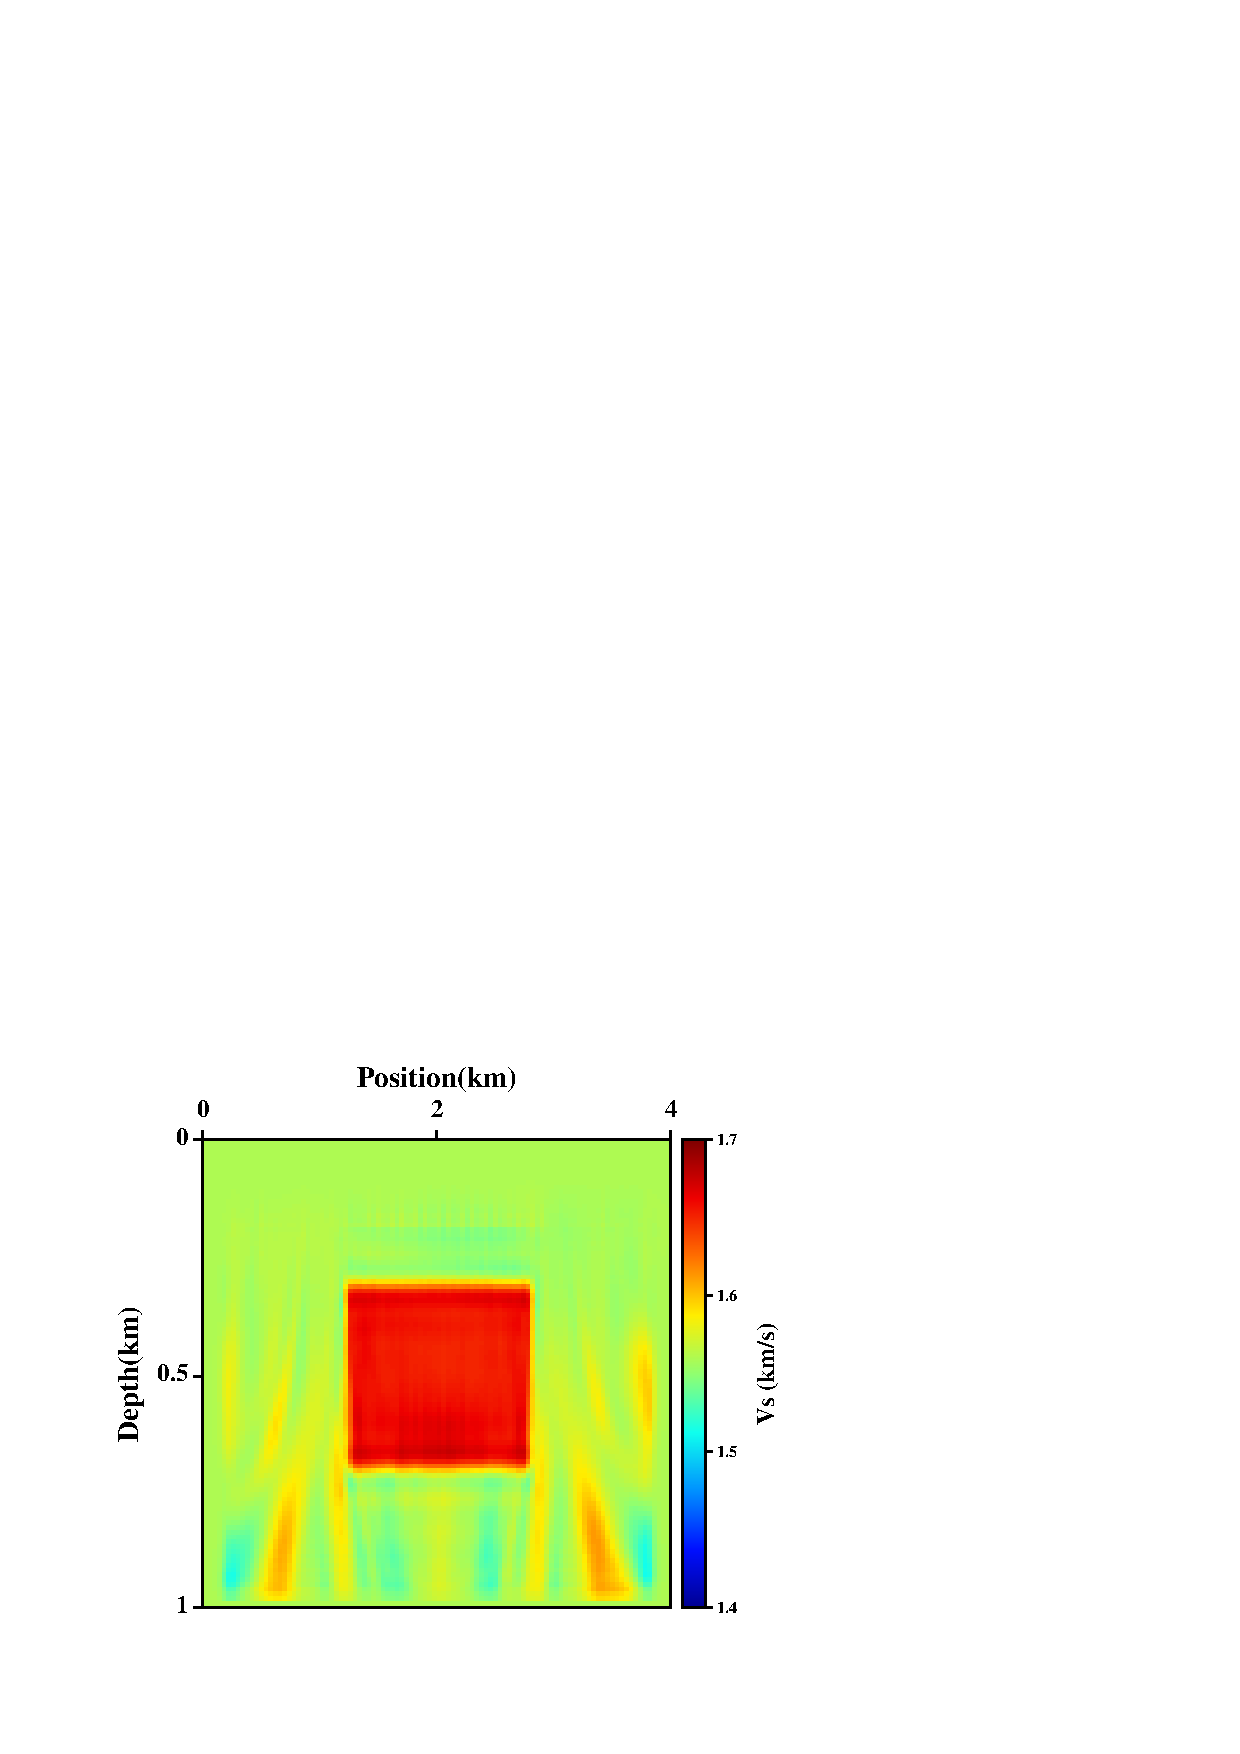
\includegraphics[width=5cm]{Figure/chapter02/smallmodel/Fig/decomvs.pdf}}
        \caption{
			流体饱和砂岩模型的EFWI结果:左侧为$V_p$,右侧为$V_s$;
			(a),(b)为真实模型;(c),(d)为常规PCG方法反演结果; (e), (f)为MDPCG方法反演结果。
    }
    \label{fig:smallmodel}
    \end{center}
\end{figure}
\subsection{Marmousi-II模型}
\begin{figure}[!htb]
    \begin{center}
		\subfloat[]{\includegraphics[width=7cm]{Figure/chapter02/tariqsugresult/Fig/truevp.pdf}}
		\subfloat[]{\includegraphics[width=7cm]{Figure/chapter02/tariqsugresult/Fig/truevs.pdf}}\\
		\subfloat[]{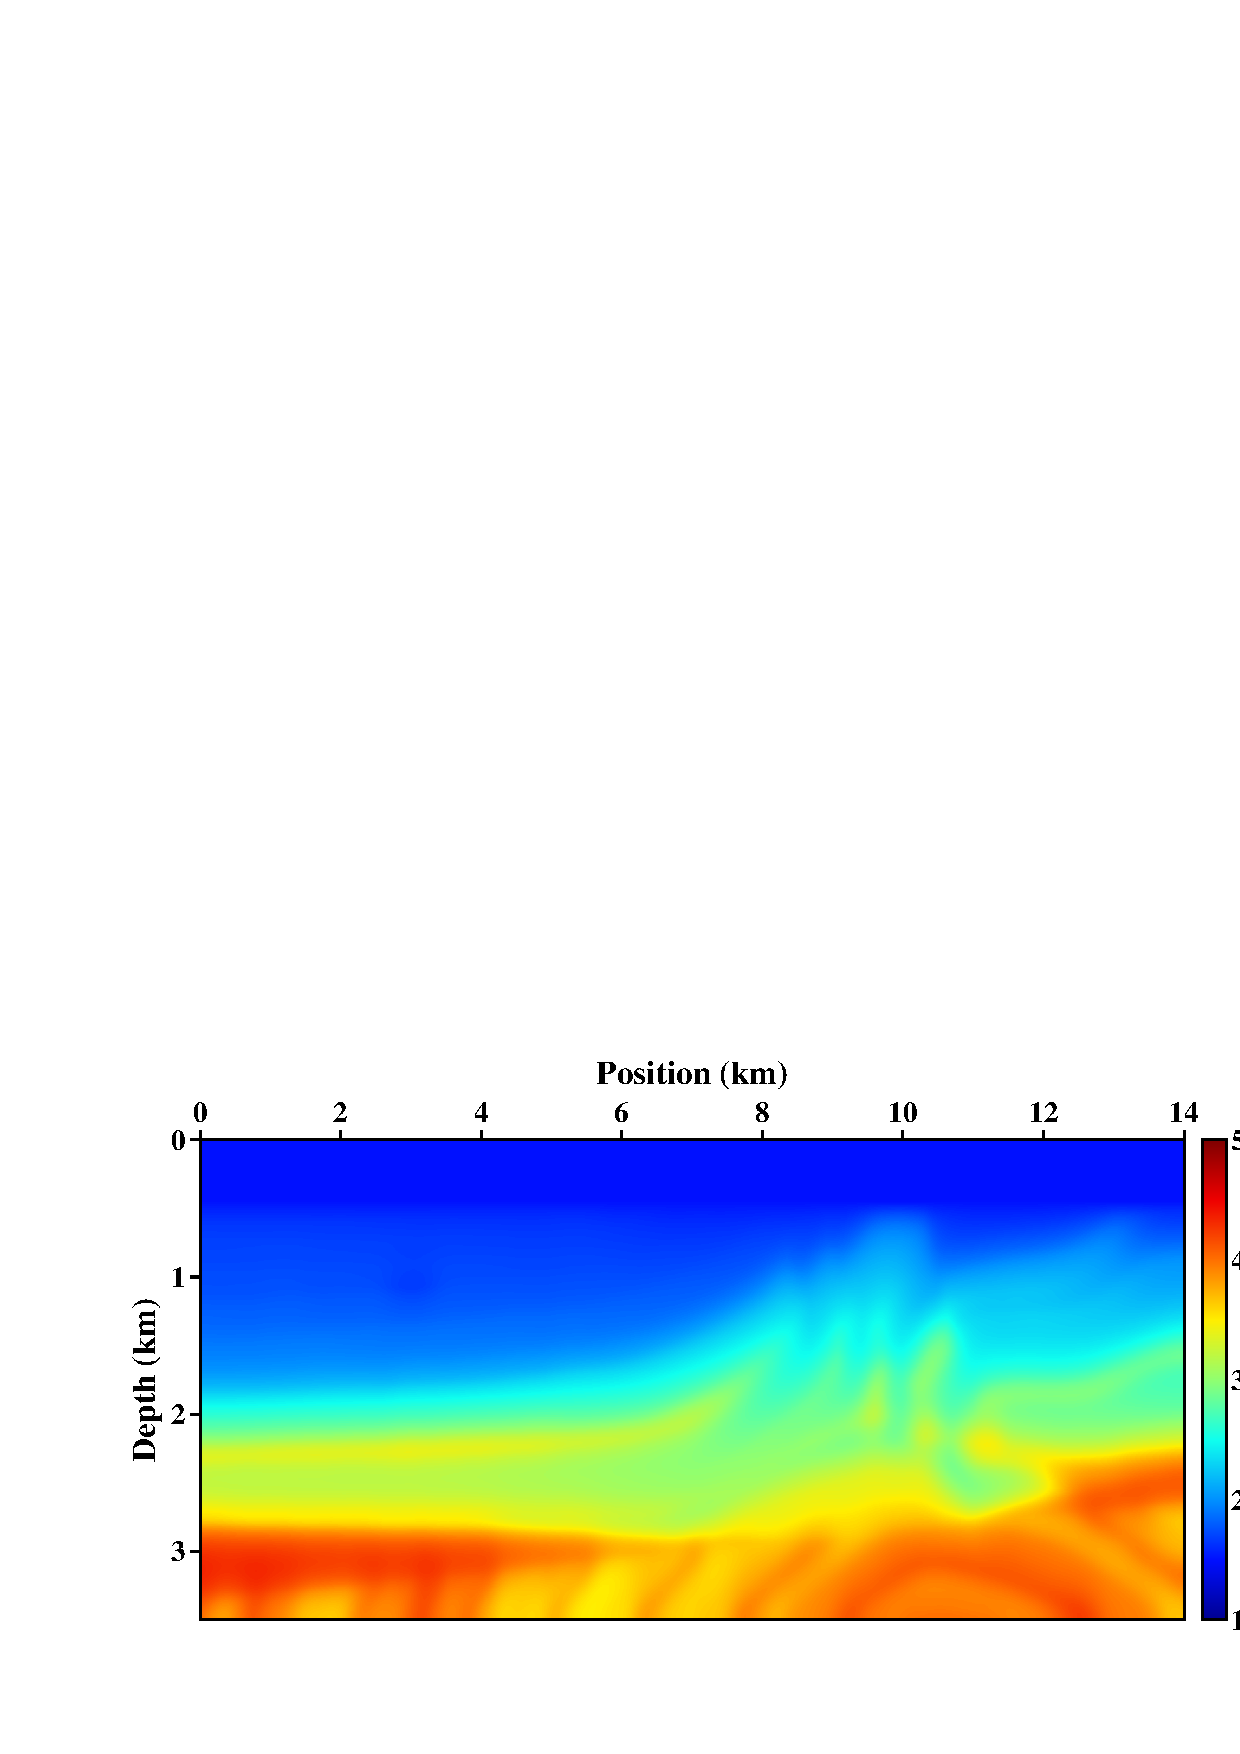
\includegraphics[width=7cm]{Figure/chapter02/tariqsugresult/Fig/initvp.pdf}}
		\subfloat[]{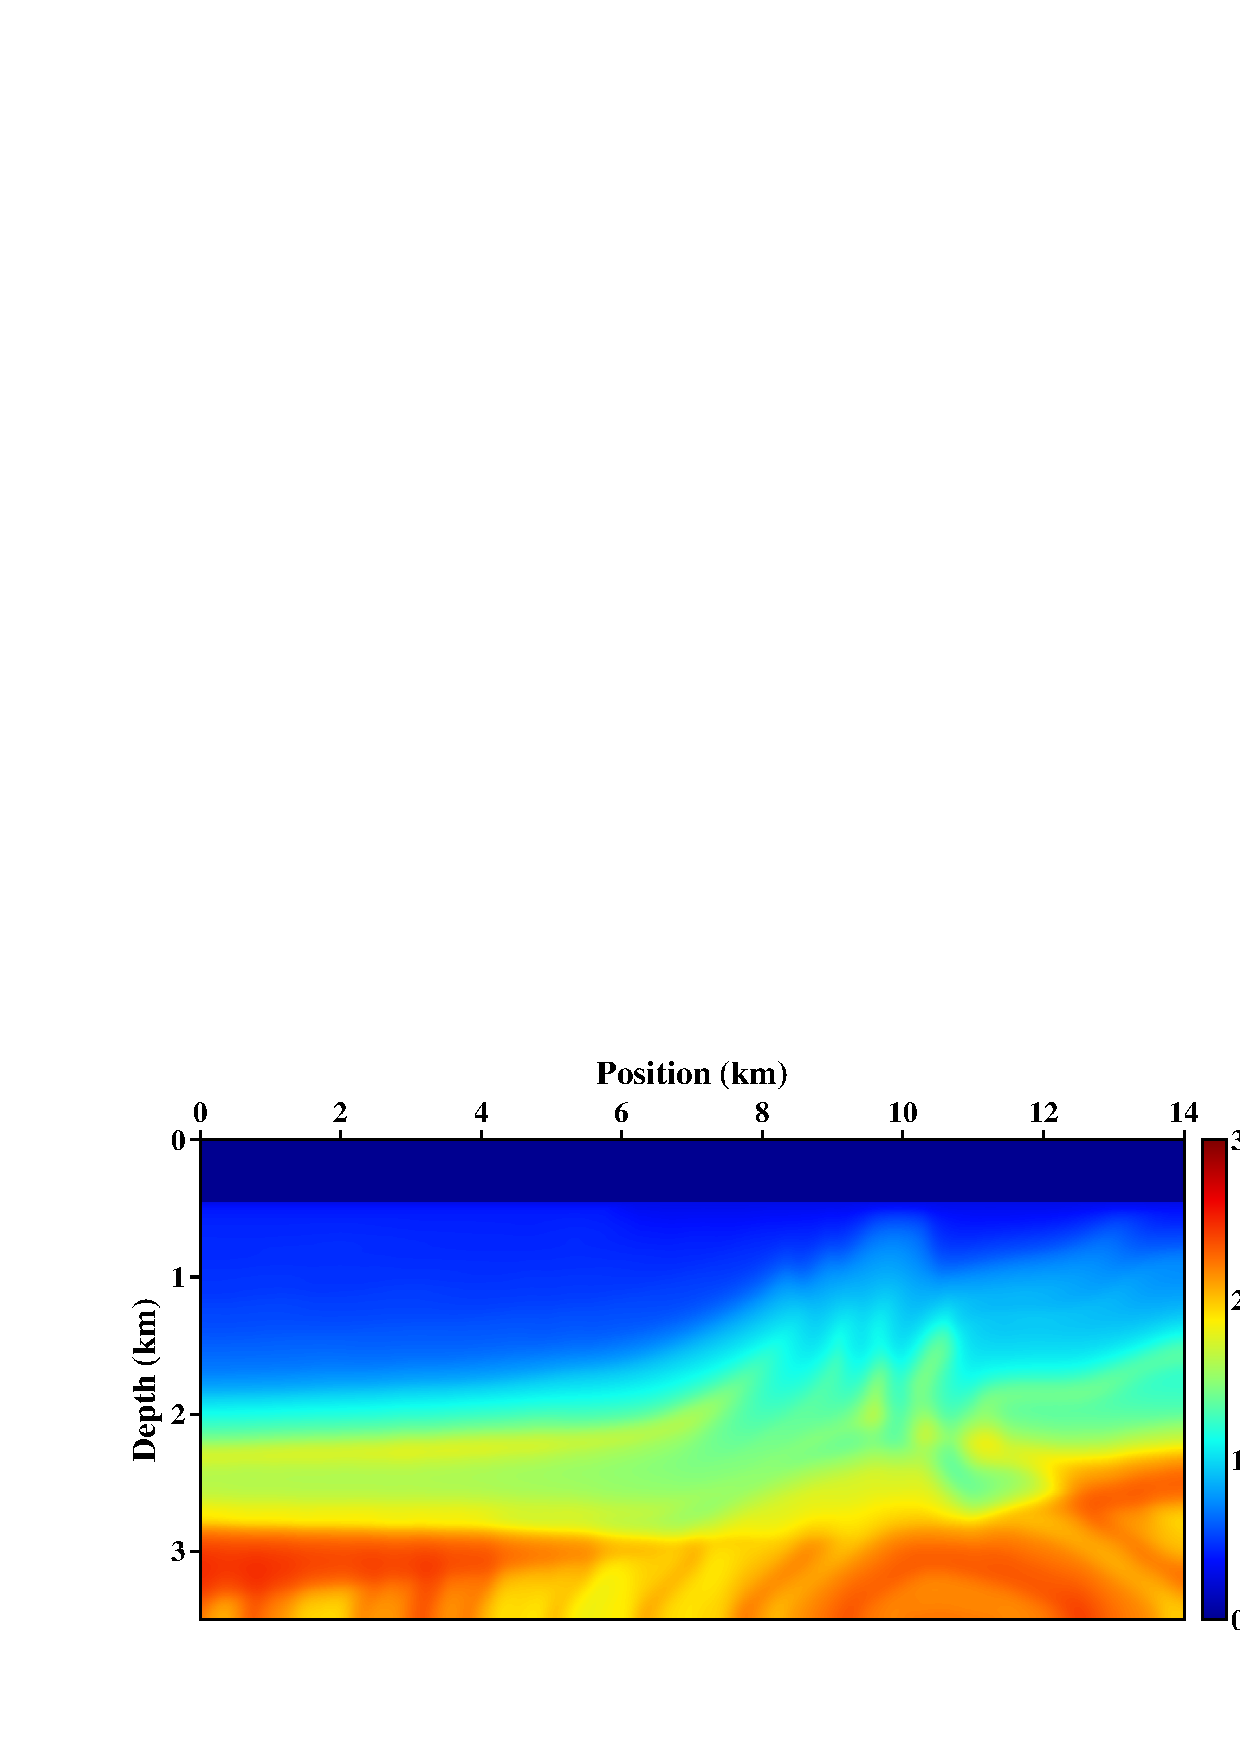
\includegraphics[width=7cm]{Figure/chapter02/tariqsugresult/Fig/initvs.pdf}}
        \caption{
			SEG Marmousii-II模型:(a), (b)分别为真实的$V_p$和$V_s$模型; (c),
			(d)分别为初始的$V_p$和$V_s$模型。注意,P波速度含有含气沙岩储层产生的速度异常以及S波速度
			中加入了高速薄层异常结构。
    }
    \label{fig:MarInitTrue}
    \end{center}
\end{figure}
\begin{figure}[!htb]
    \begin{center}
		\subfloat[]{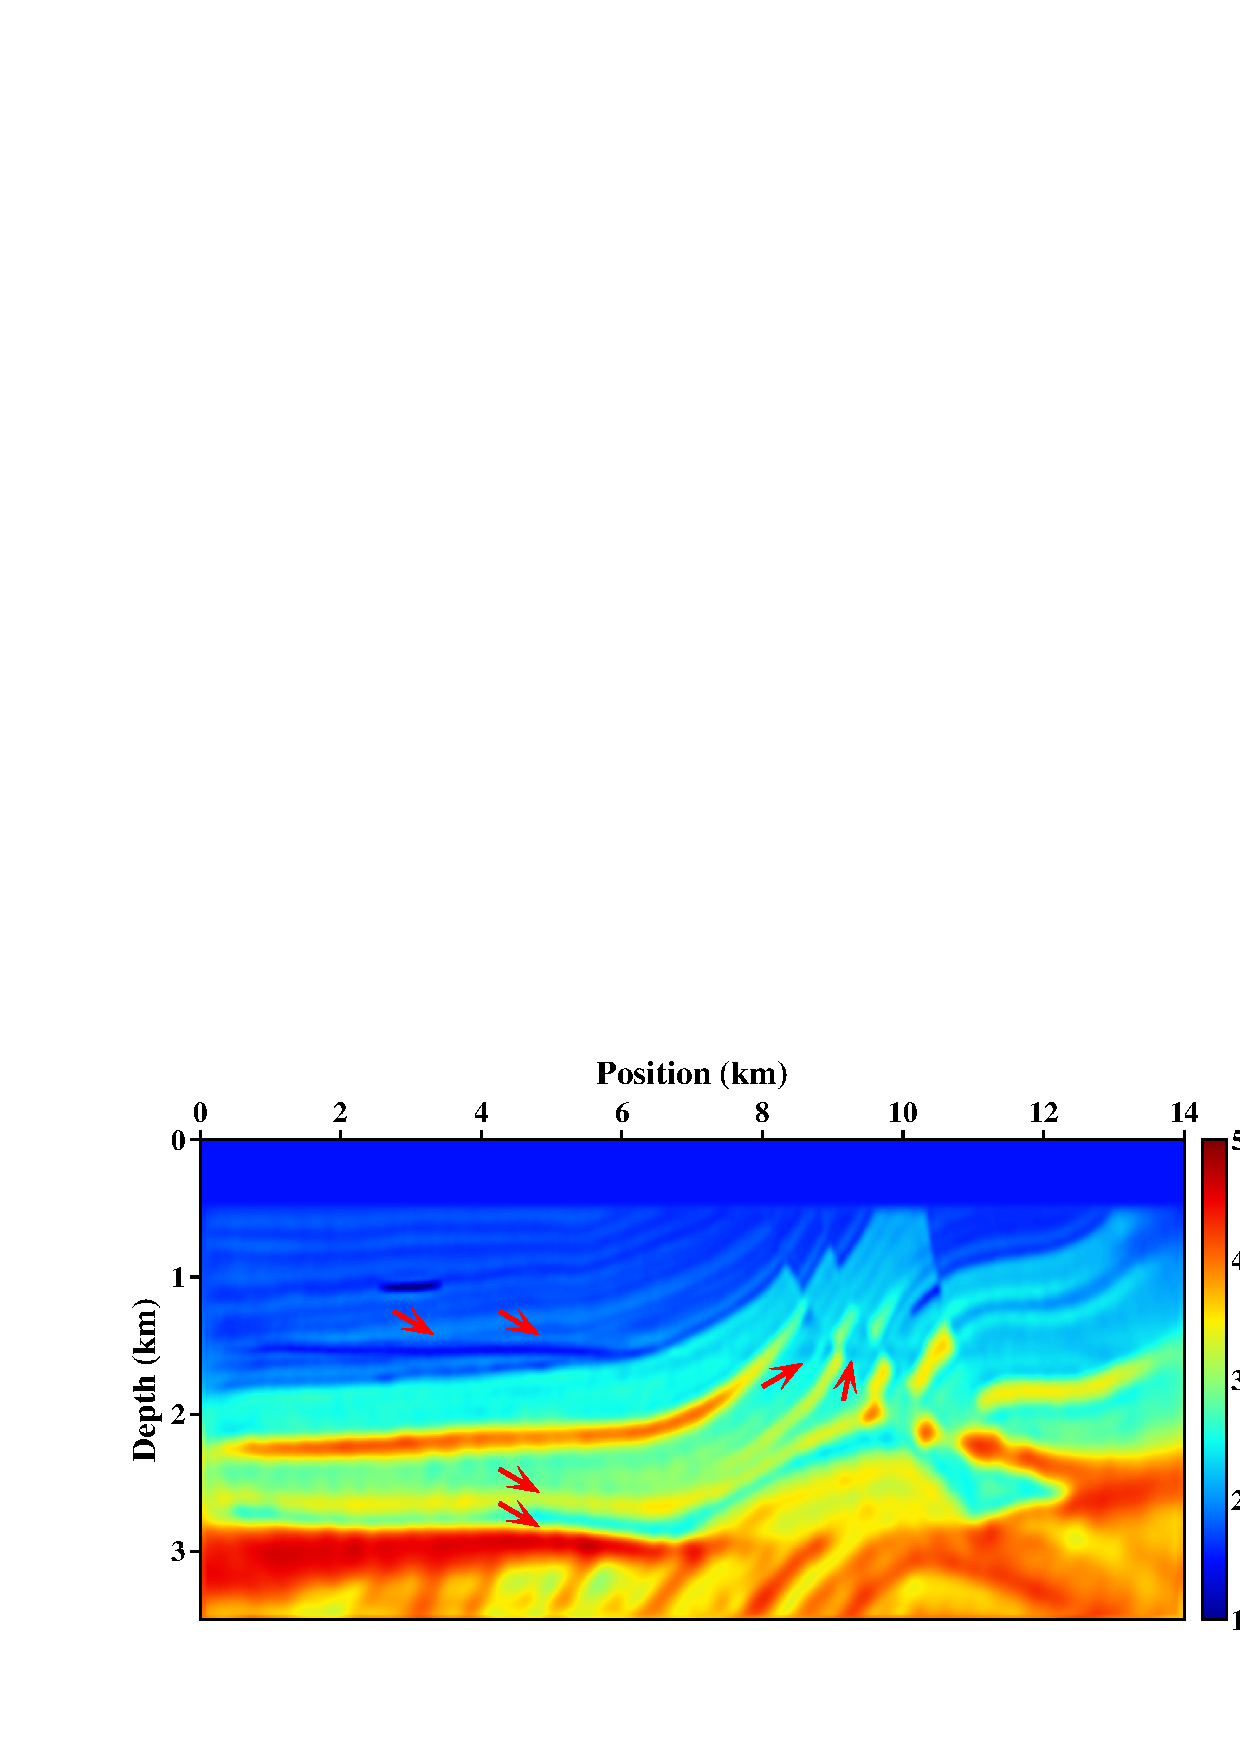
\includegraphics[width=7cm]{Figure/chapter02/tariqsugresult/Fig/nodevp.pdf}}
		\subfloat[]{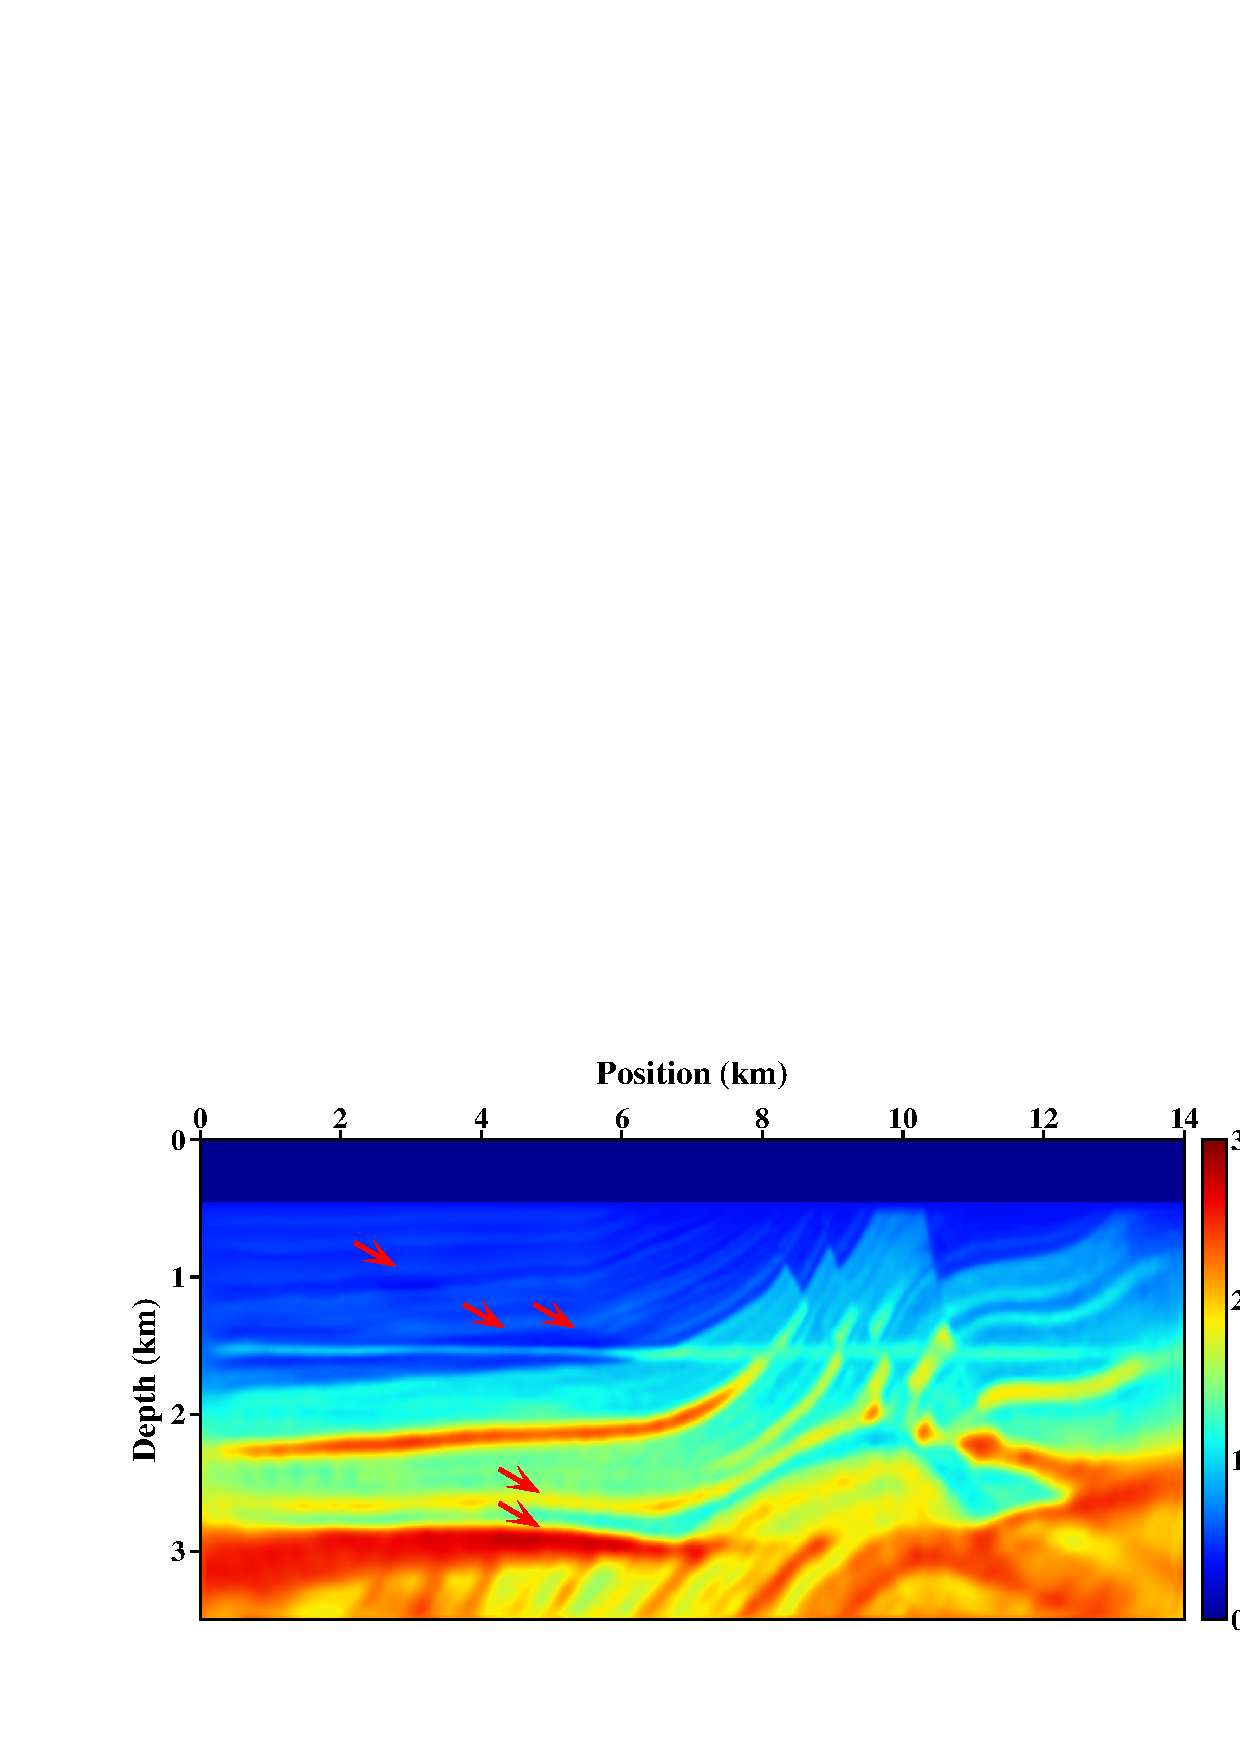
\includegraphics[width=7cm]{Figure/chapter02/tariqsugresult/Fig/nodevs.pdf}}\\
		\subfloat[]{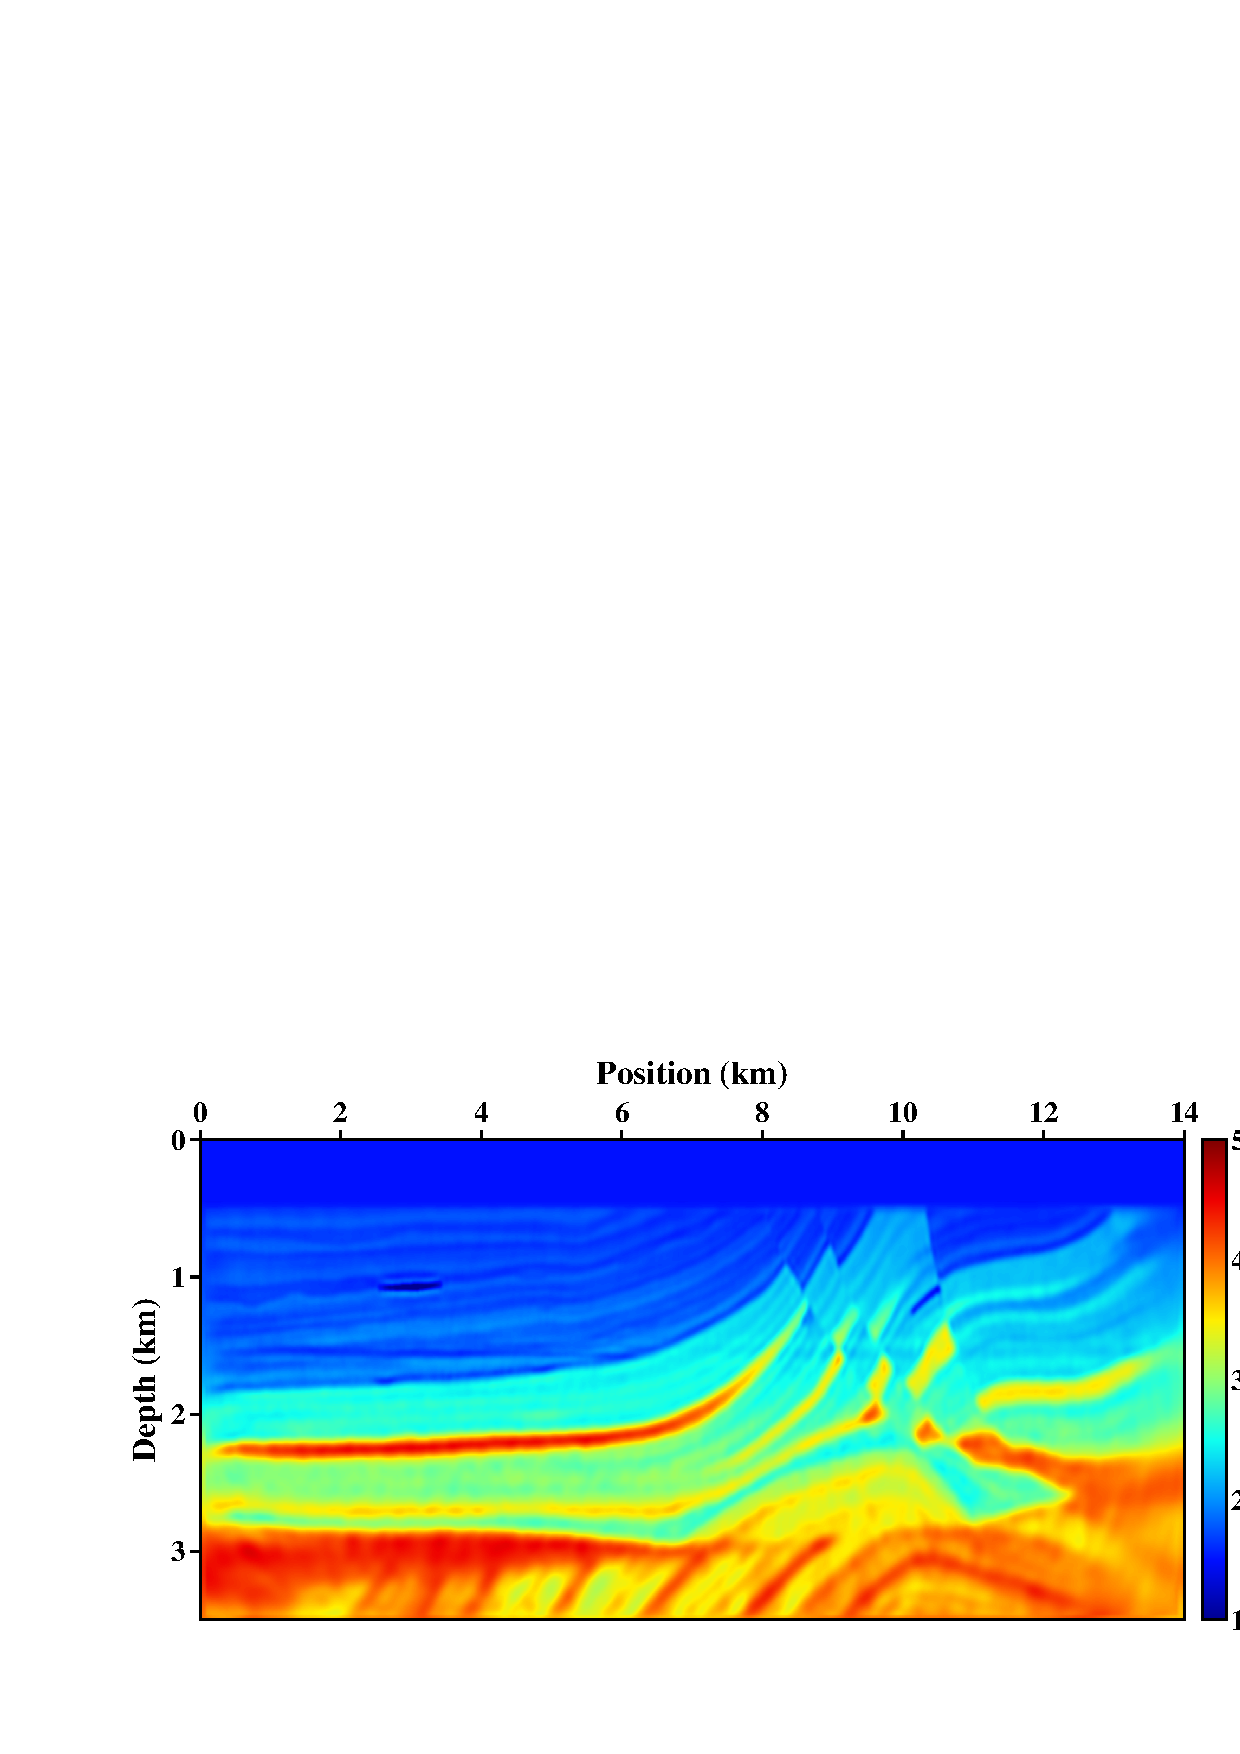
\includegraphics[width=7cm]{Figure/chapter02/tariqsugresult/Fig/devp.pdf}}
		\subfloat[]{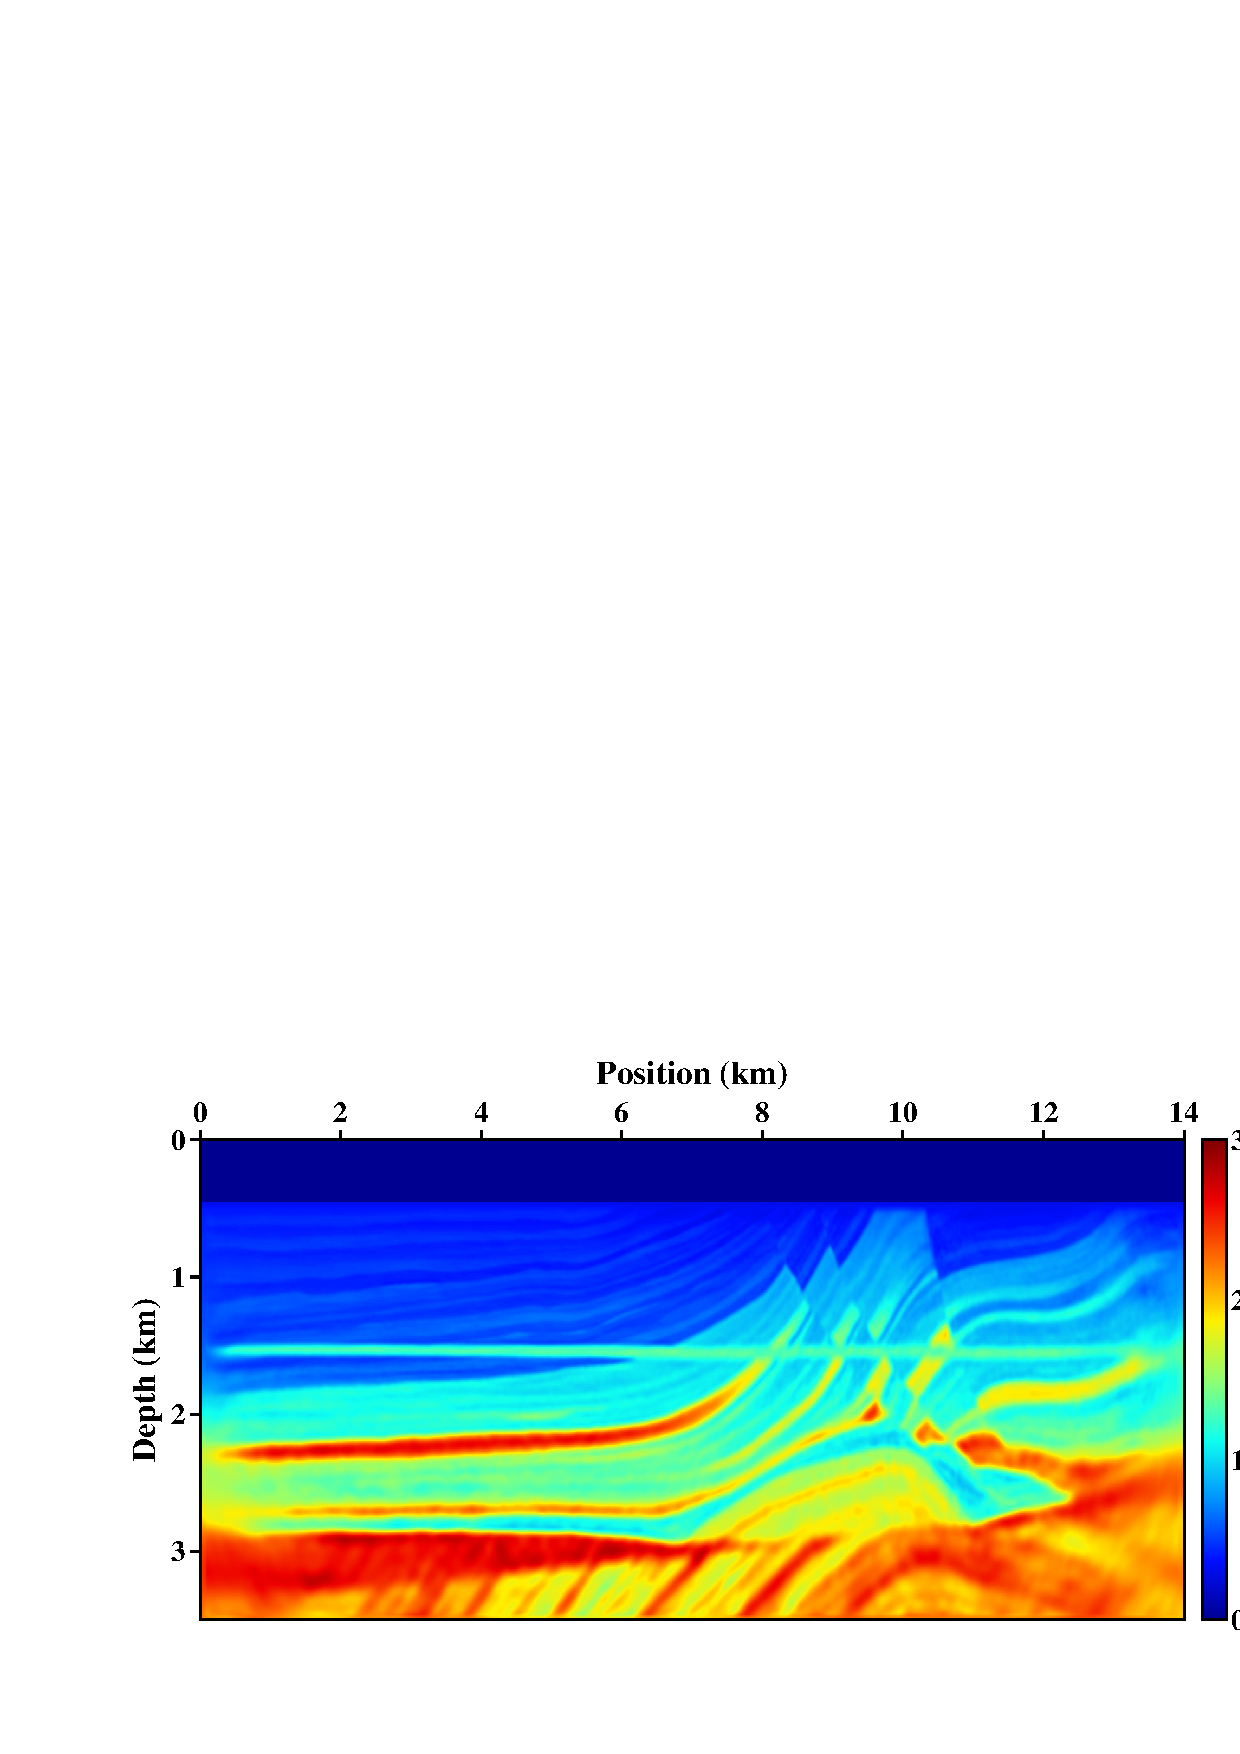
\includegraphics[width=7cm]{Figure/chapter02/tariqsugresult/Fig/devs.pdf}}
        \caption{
			反演的Marmousi-II模型:其中左侧为$V_p$,右侧为$V_s$. (a), (b)为常规PCG方法反演结果;(c), (d)为MDPCG方法反演结果。
%        The inverted Marmousi-II model: The inverted results using the PCG (a, b)
%            and the MD-based methods (c, d).
%        (a) and (c) are $V_p$ models while (b) and (d) are $V_s$ models.
    }
    \label{fig:MarInvert}
    \end{center}
\end{figure}
过去十年间,很多EFWI策略被用在了OBC地震数据中。在地震数据低频成分比较丰富的情况下,重建低Poisson比的模型(如硬海底)相对比较容易\cite[]{bae:2012}。
然而,软海底环境在现实中更为普遍。此时,PS转换能量非常有限,反演中的非线性程度以及参数间的耦合也
会变得更加严重。为了应对这种更真实的软海底情况,
如图\ref{fig:MarInitTrue}(a)和(b)所示,用Marmousi-II模型中的原始P波与S波速度来测试算法。不同参数间非一致的结构能更明显地调查参数间的耦合程度。
为了更好的展示本文方法的优势,在S波速度模型1.5km深处添加了一个高速的薄层。在反演中,我们采用交错网格有限差分法来计算正传与共轭波场,空间采样间隔为5m,
记录总时间为8s,时间采样间隔为0.5ms。共有40炮合成数据,炮点深度在20m的水深处,2800个检波点放置于海底来模拟OBC观测。初始模型通过SU软件中的smooth2函数
平滑真实模型产生,平滑半径为300m。采用与前一实验同样的多尺度策略,但是每阶段最大迭代次数扩大为40次。

图\ref{fig:MarInvert}的结果表明了MDPCG方法比常规PCG方法能提供更好的反演结果。
在模型浅部(约1.5km),两种方法都能很好的恢复$V_p$模型,而常规方法恢复的$V_s$模型
分辨率较低。S波速度模型中的高速异常薄层给反演造成了很大的挑战,如图\ref{fig:MarInvert}(a)和(b)中所示,反演结果存在很强的参数耦合
的干扰,尤其是在左侧的高速异常薄层附近。这就导致了该异常薄层下方构造的错位与不聚焦(如图中箭头所示)。然而,MDPCG方法很好地压制了这些参数耦合效应,
获得了模型的许多细节,包括中部的断层与背斜构造。模型的纵向“测井”曲线(图\ref{fig:VertiProfile})
进一步证明了模式解耦反演方法获得了比常规方法更准确的结果与更高的分辨率。
\begin{figure}[!htb]
	\begin{center}
		{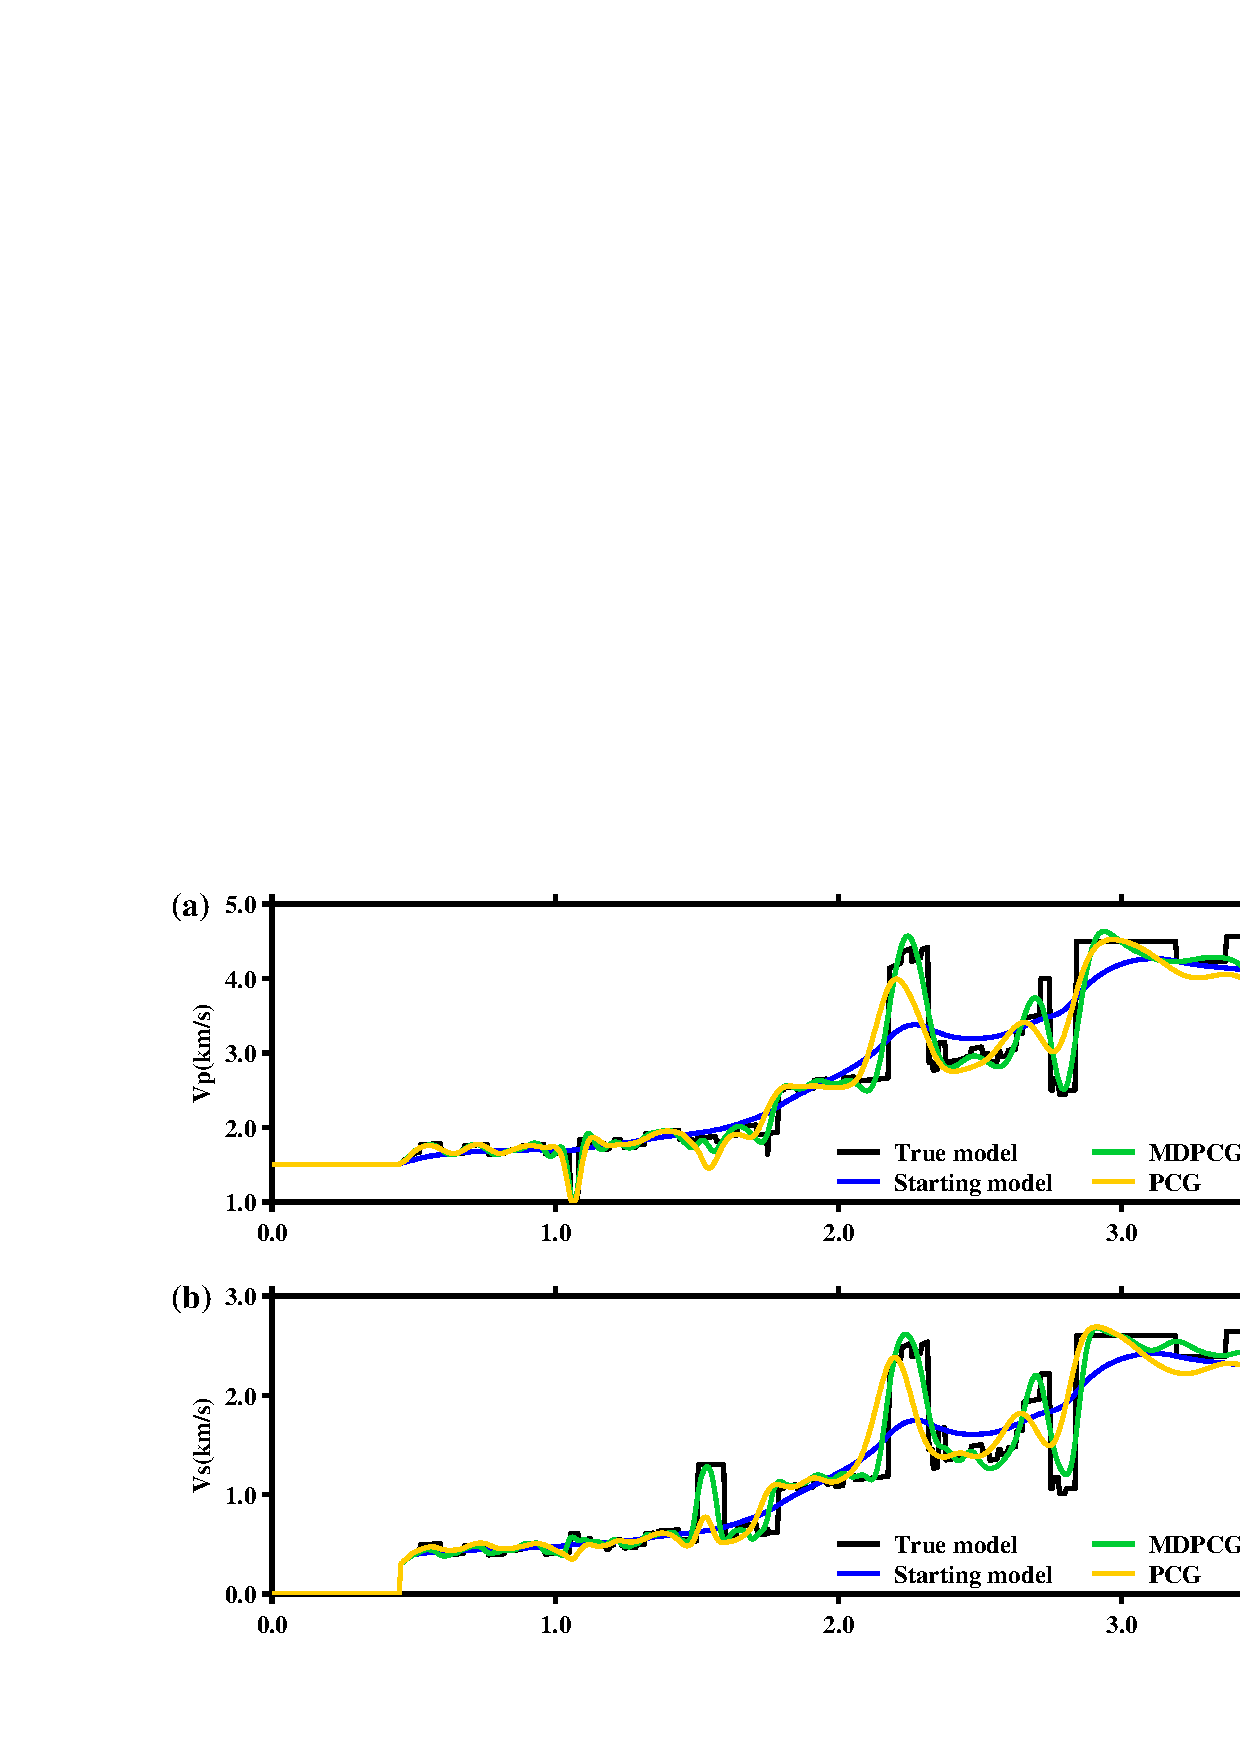
\includegraphics[width=10cm]{Figure/chapter02/tariqsugresult/Fig/new3km.pdf}}
		{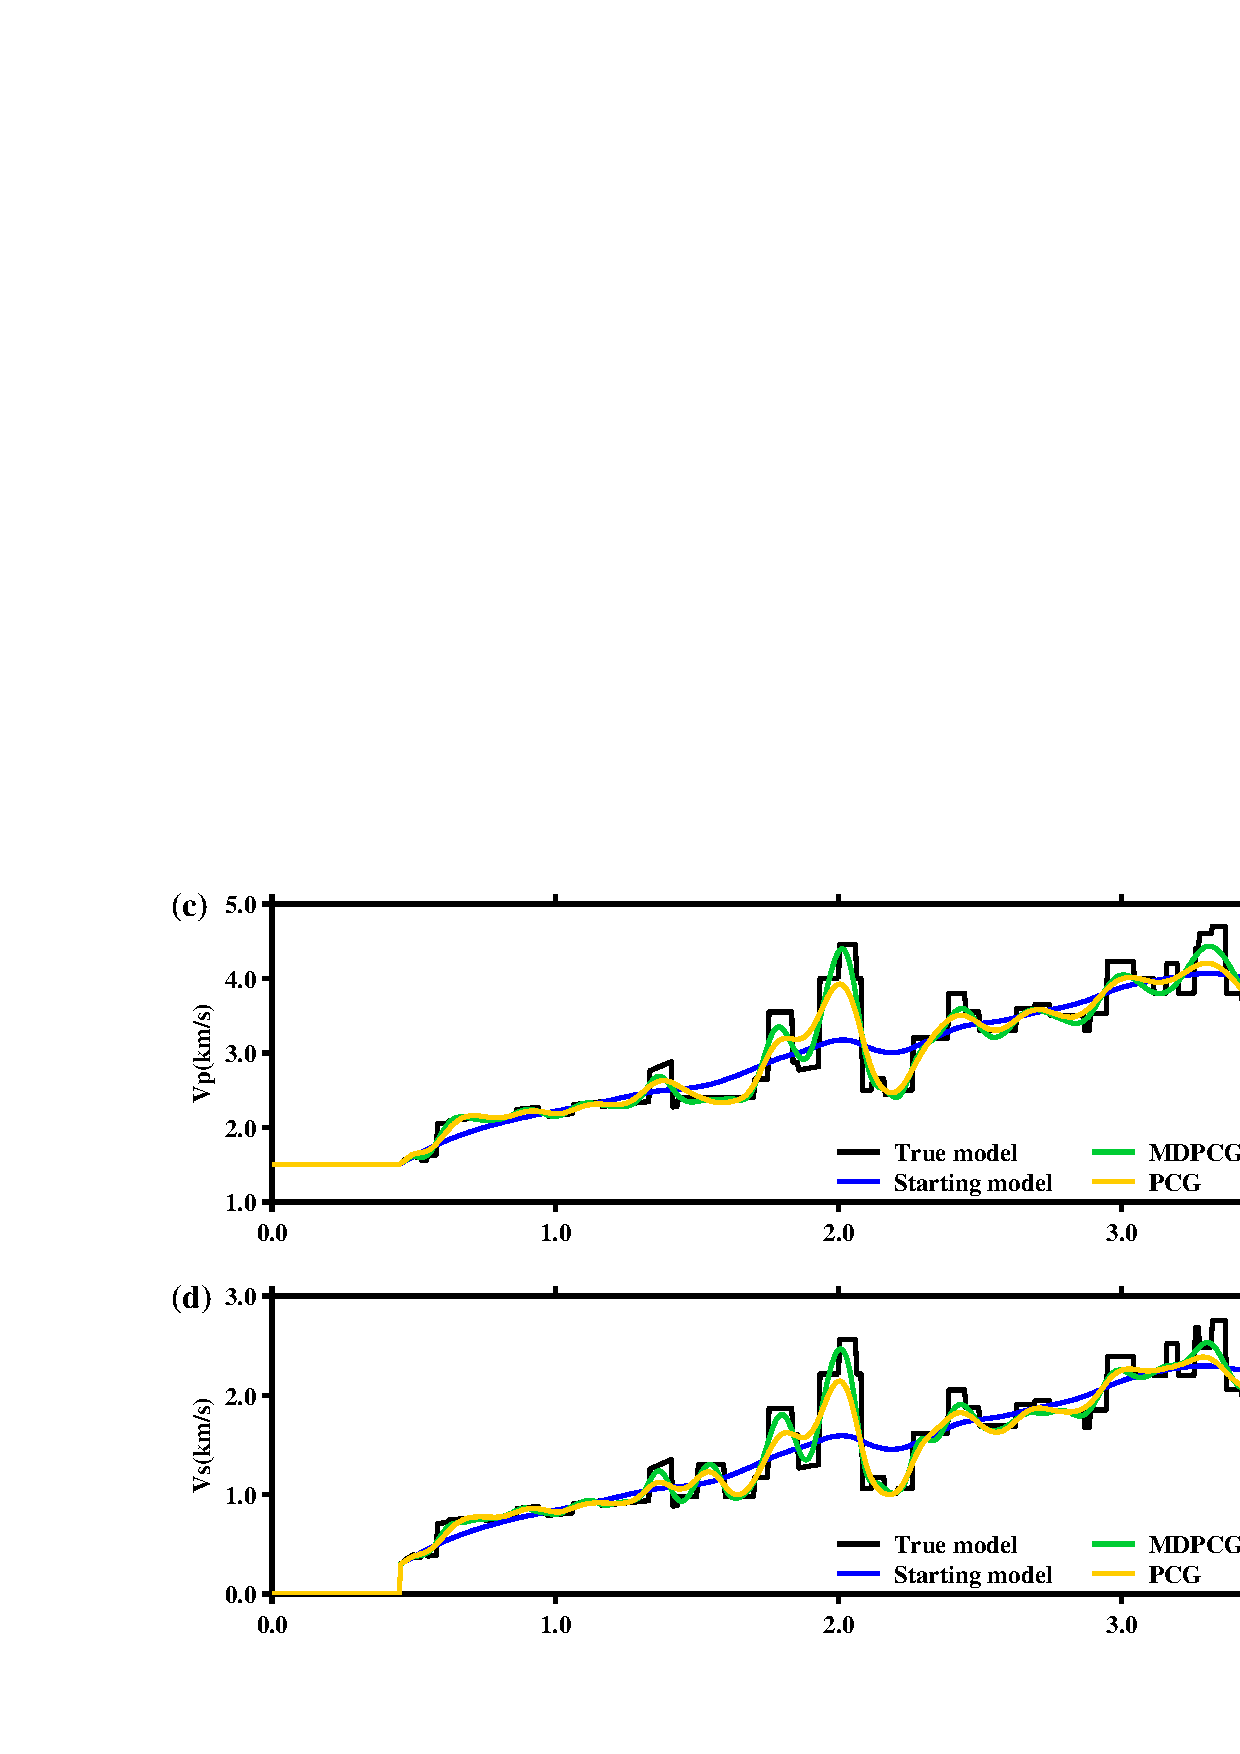
\includegraphics[width=10cm]{Figure/chapter02/tariqsugresult/Fig/new9km.pdf}}
		\caption{
		模型在3.0km(a,b)和9.0km(c,d)处的纵向剖面。黑线和蓝线分别代表真实和初始模型;黄线与绿线分别代表常规PCG和MDPCG方法反演结果。
%		The velocity profiles at 3.0 km (a, b) and 9.0 km (c, d) with the true models
%			(black),
%			the initial models (blue), the PCG-based (yellow) and MD-based (green)
%			inverted models.
	}
	\label{fig:VertiProfile}
	\end{center}
\end{figure}

\begin{figure}[!htb]
    \begin{center}
        \includegraphics[width=10cm]{Figure/chapter02/tariqsugresult/Fig/L2.pdf}
        \caption{
			归一化后的L2残差随迭代次数的变化。红色与蓝色代表第一和第二阶段的反演,虚线代表常规PCG方法
			实线代表MDPCG方法。
%            Normalized L2 norms as a function of iteration for the PCG-based (dash)
%            and MD-based (solid) inversions in the first (red) and second (blue)
%            stages.
    }
    \label{fig:L2}
    \end{center}
\end{figure}
图\ref{fig:L2}展示了在前两个阶段的反演中,归一化的目标函数值随迭代次数的下降曲线。可以看到,MDPCG方法要比常规PCG方法收敛更快。在第一个阶段,模式解耦
反演方法的数据拟合程度更高,获得了更准确的中低波数模型更新。在第二个阶段,常规PCG方法最终在25次迭代之后停止更新且数据残差仍相当大,而MDPCG方法
在22次迭代后数据残差快速下降达到终止条件。这些分析表明利用模式解耦对梯度做预条件可以很有效地在反演中降低参数耦合从而加速收敛。
\begin{table}[!htb]
    \caption{计算时间对比}
    \label{table:TotalComputime}
	\centering 
%   \begin{tabular}{|c|c|c|c|c|c|c|}
%   \begin{tabular}{|p{1.8cm}|c|c|c|c|p{2.2cm}p{2.3cm}p{2cm}|}
    \begin{tabular}{p{1.8cm}p{1.0cm}p{1.0cm}p{1.0cm}p{1.2cm}p{1.0cm}p{1.0cm}}
%    \begin{tabular}{|p{1.8cm}|p{1.0cm}p{1.0cm}p{1.0cm}p{1.2cm}|p{1.0cm}p{1.0cm}|}
    \hline
    \quad&\multicolumn{4}{c}{Iteration number}&\multicolumn{2}{c}{Time spent (hour)} \\
%   \quad&\multicolumn{4}{|c|}{Iteration number}&\multicolumn{2}{|c|}{Computing Time (hour)} \\
    \hline
%   Method & stage1 0-2Hz &stage2 0-4Hz&stage3 0-6Hz&stage4 0-10Hz&Total &Average \\
    \multirow{2}{*}{Method} & stage1 &stage2 &stage3 &stage4 &\multirow{2}{*}{Total}
    &\multirow{2}{*}{Average} \\
    & 0-2Hz &0-4Hz&0-6Hz&0-10Hz\\
    \hline
    Conventional&  40   &25&5& 7  &41.4&0.538\\
    MD-based &   40  & 22 &33 &13&68.3&0.632\\
    \hline
    \end{tabular}
\end{table}

表\ref{table:TotalComputime}
中列出了在8节点(每节点15核)的工作站上每个阶段的迭代次数和总的计算时间。每个阶段我们设定最大迭代次数为40次。因为当搜索不到合适步长的时候迭代会自动终止,所以
不同阶段的实际迭代次数并不相同。在常规方法中,严重的参数耦合效应会影响从低频数据中重建出合适的宏观模型,这就导致在高频阶段无法获得合理的梯度方向,使得迭代过早终止。而MDPCG方法可以一定程度压制参数耦合,在低频阶段能够重建出合适的宏观模型,从而使得高频阶段的梯度更合理。这也是为什么模式解耦方法能
获得更准确、分辨率更高的反演结果。总的来说,模式解耦方法需要更多的迭代次数,也因此耗费更多计算时间。就本例而言每次迭代的平均用时只增加了18\%左右。
\section{讨论}
\subsection{更进一步分解梯度的必要性}
理论上讲,可以对正传与反传波场分别解耦从而获得对应不同模式转换(也即PP、PS、SP和SS)的解耦梯度。但是,很难设计出一个单独使用某一模式转换数据的EFWI方法,因为地面
P/S分离算法无法区分入射波场的类型,即无法区分PP与SP(或PS与SS)。不然只能使用分解后的单模式地震数据来进行单参数反演。例如
Ren和Liu\cite{ren.liu:2016},在其四步反演策略的第二步中,当有很强的S波能量时,只采用分解的P波场来反演P波速度,或者在弱S波能量时仅仅拟合S波数据来反演S波速度。


需要注意的是,在梯度计算中正传波场解耦等价于次级源(或背景波场)的波模式解耦,而次级源又是Frech{$\acute{e}$}t导数中的一部分。因此可以将该线性问题写为:
\begin{equation}
    \mathbf{J}^{XY}\delta\mathbf{m}=\mathbf{\delta u}^{XY},
    \label{eq:JXY}
\end{equation}
其中$X$和$Y$分别表示次级源与散射Green's函数的波模式,$\mathbf{\delta u}^{XY}$则表示${X}{Y}$模式的扰动波场。根据方程\eqref{eq:ResoOperP}的推导方式,
可以获得相应的分辨率矩阵:
\begin{equation}
    \mathbf{R}^{XY}=\mathbf{H}_a^{-g}\mathbf{J}^{\dagger}\mathbf{J}^{XY}. 
    \label{eq:RXY}  
\end{equation}
图\ref{fig:ResoMN}展示了PP、PS、SP和SS模式的分辨率矩阵,其观测系统与图\ref{fig:Resolution}中一致,但是采用了P和S波的混合震源。图中的带对角形式是由于更加复杂的
波现象。可以看到,$\mathbf{R}^{PP}$ 与$\mathbf{R}^P$十分类似,而$\mathbf{R}^{SP}$却几乎为空矩阵。这表明用PP波数据来反演$V_p$会受到来自$V_s$的干扰。而SP波数据
则对两个参数的反演贡献都很小。从Ren和Liu\cite{ren.liu:2016}的例子中(见其文中图19与20),即使震源中含有足够强的S波能量,SP梯度也很弱且有很多噪音。一个
可能的解释就是如图\ref{fig:SPSS}所示,SP的散射能量很弱。此外,也难以
区分出PS和SS模式各自的贡献,因为从图\ref{fig:ResoMN}中看到,$\mathbf{R}^{PS}$和
$\mathbf{R}^{SS}$的非零元素分布非常一致。因此,通过正传波场解耦来进一步压制参数耦合效应的潜力非常有限,尽管这样会带来更多的计算量。这也是为什么本文只
分解反传波场来对梯度进行预条件。
\begin{figure}[!htb]
    \begin{center}
        \includegraphics[width=12cm]{Figure/chapter02/ResoOpera/Fig/resolutionMN.pdf}
        \caption{
			采用混合震源时不同模式数据转换的分辨率矩阵。
%            Resolution matrices associated with different mode conversion data using
%            mix-source:
            (a) $\mathbf{R}$, (b) $\mathbf{R}^{PP}$, (c) $\mathbf{R}^{PS}$, (d)
            $\mathbf{R}^{SP}$ 和(e)
            $\mathbf{R}^{SS}$.
    }
    \label{fig:ResoMN}
    \end{center}
\end{figure}

\begin{figure}[!htb]
    \begin{center}
        \includegraphics[width=5cm]{Figure/chapter02/radiationpattern/Fig/SPSS.pdf}
        \caption{
			归一化的SP模式(红色)和SS模式(蓝色)的辐射模式。
%            Radiation pattern of SP and SS modes with a same normalization: SP
%            mode (red) and SS mode (blue).
    }
    \label{fig:SPSS}
    \end{center}
\end{figure}
\subsection{密度模型的反演}
密度扰动同时散射P和S波,但是却几乎不影响两种波模式的相位或者走时。这些模式的散射能量大多与入射波场的传播方向相反\cite[]{wu.aki:1985,tarantola:1986}。因此,
密度作为一个次级效应参数,由于其微弱的敏感性和多参数的耦合效应\cite[]{tarantola:1986,forgues.lambare:1997},很难被准确重构。这也是为何很多EFWI的研究只考虑
常密度的情形\cite[]{shipp:2002,sears2008,brossier2009}。只有很少一部分的工作能够利用多尺度策略和(或)不同参数化方式的选取中获得较为合理的密度反演结果
\cite{jeong2012full}。最近,基于子空间方法\cite[]{kennett:1988},Xu和McMechan\cite{xu.mcmechan:2014}提出了一种多步长的梯度类方法来压制$V_p$, $V_s$和
$\rho$之间的串扰。Yang等\cite{Yang2016}采用改进的散射积分法(SI)通过Hessian的逆来改善声波FWI中$V_p$和$\rho$的估计。尽管Ren和Liu\cite{ren.liu:2016}提出了
基于波场解耦的四阶段多尺度策略来做EFWI,但是他们只是在第二阶段中采用了P/S分离来压制$V_p$和$V_s$之间的耦合,然后通过多步长的手段来改善三参数同时反演的效果。
在他们展示的overthrust模型中,密度的反演结果仍然偏离真实模型较远。因此,非常有必要进一步调查模式解耦预条件方法对改善密度反演的潜力。
\begin{figure*}
    \begin{center}
        \subfloat[]{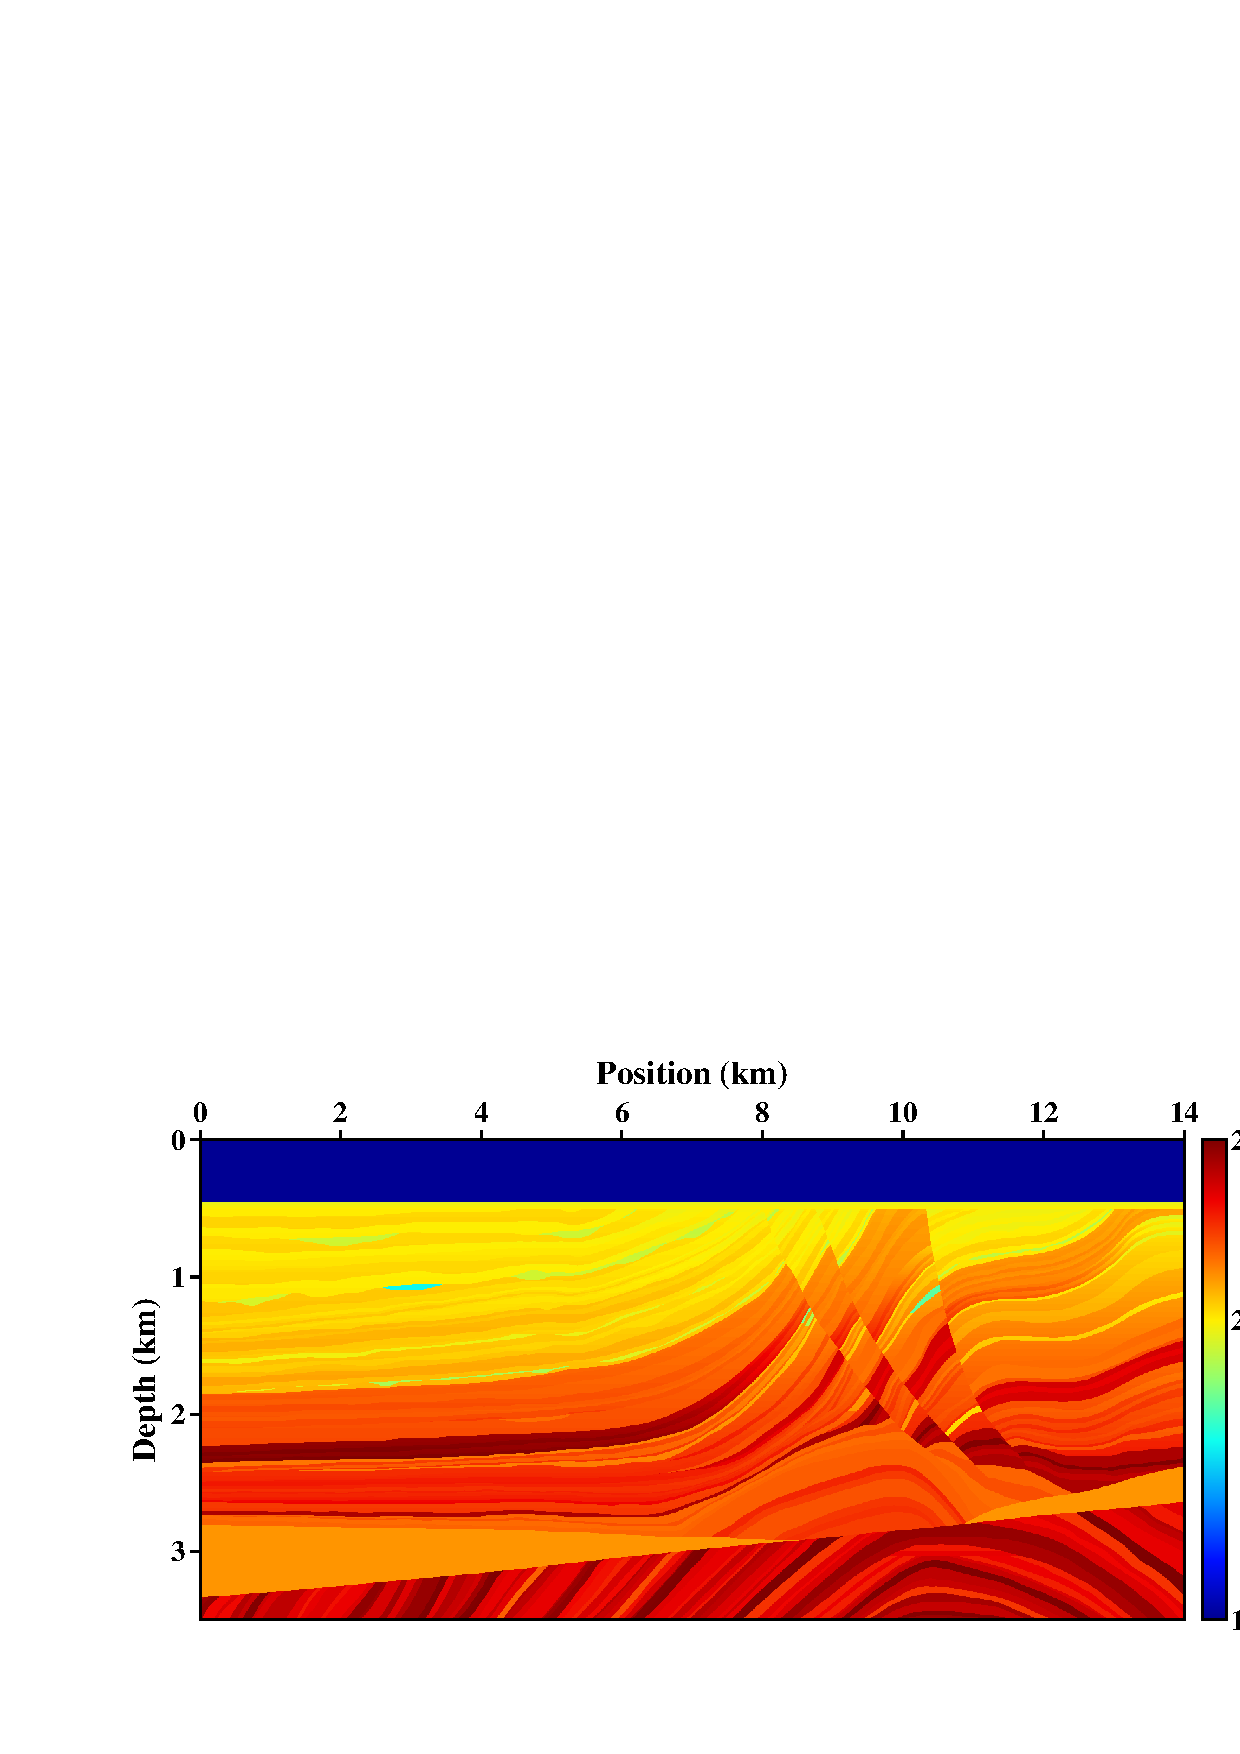
\includegraphics[width=7cm]{Figure/chapter02/tariqsugresult/Fig/truerho.pdf}}
        \subfloat[]{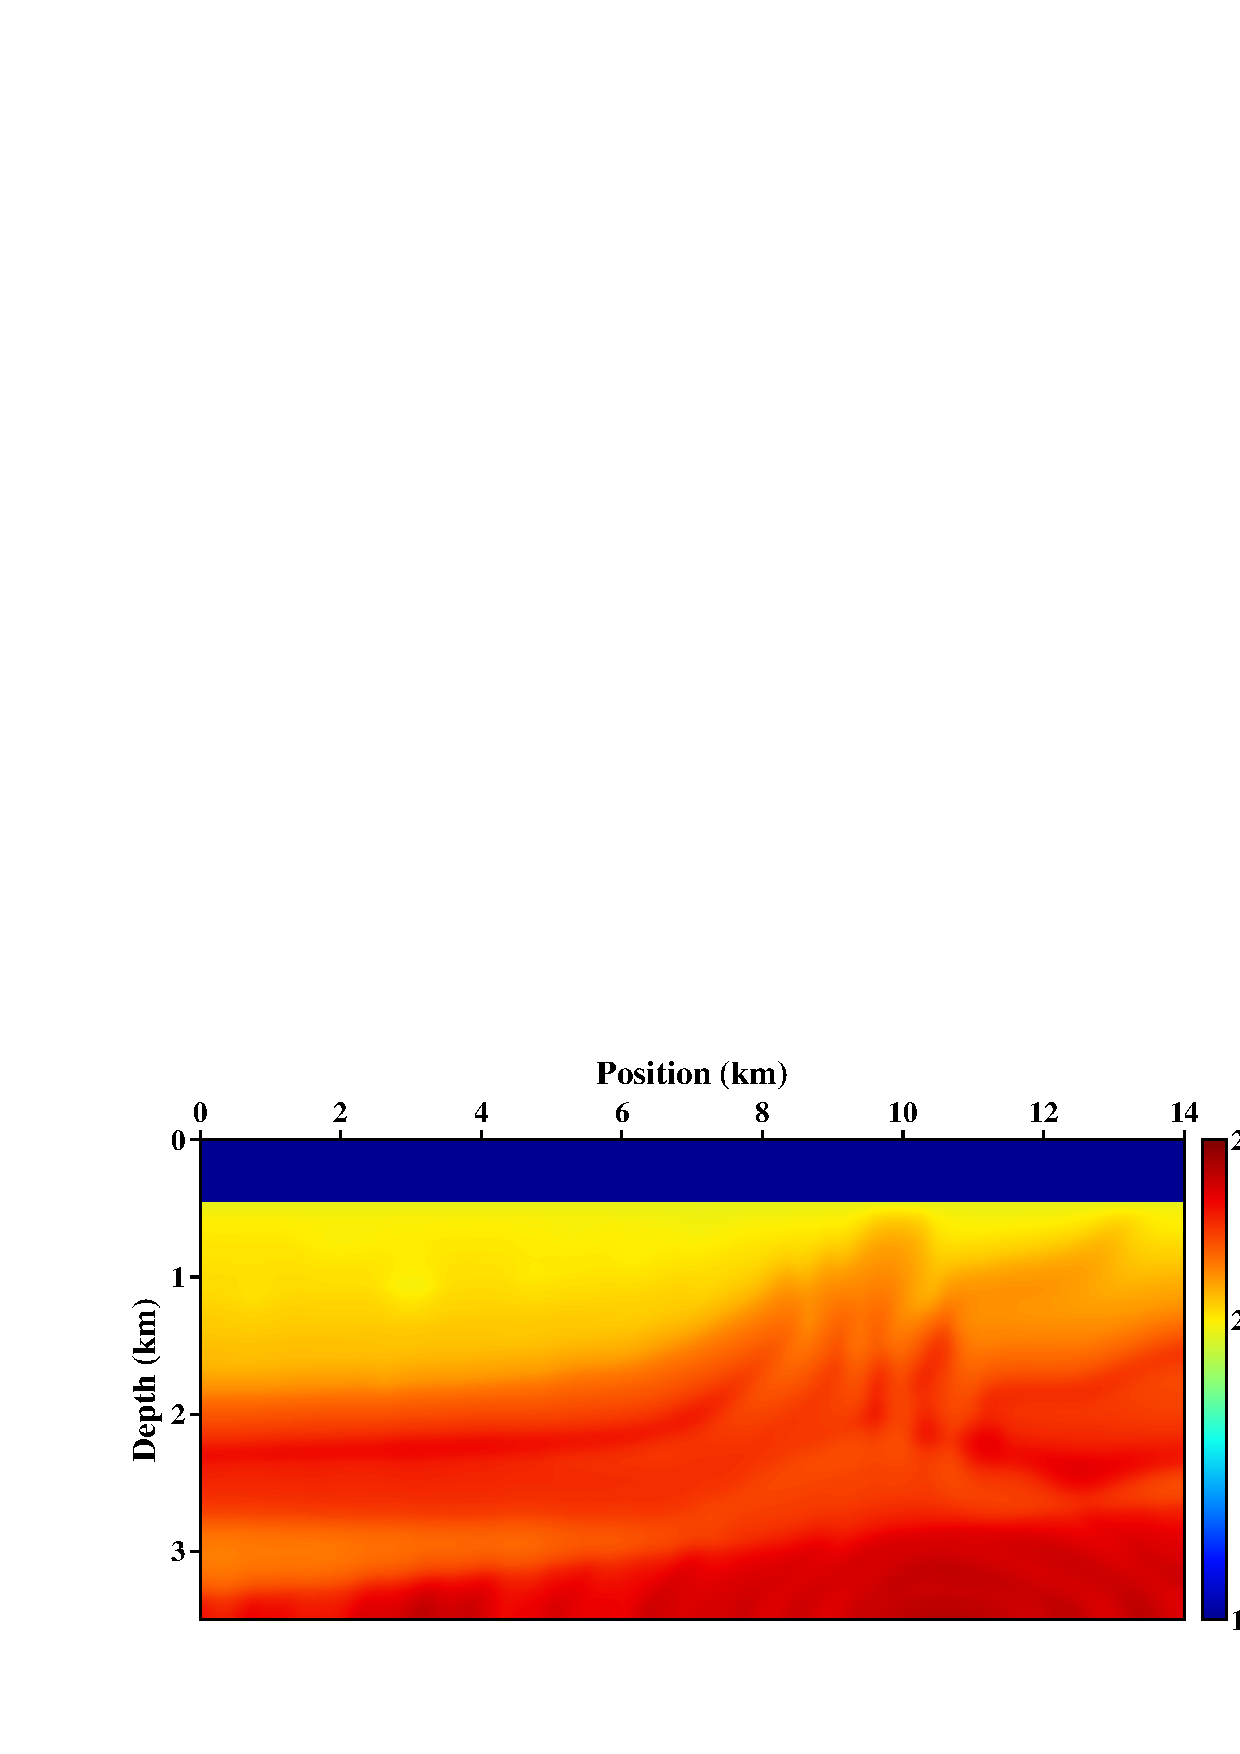
\includegraphics[width=7cm]{Figure/chapter02/tariqsugresult/Fig/initrho.pdf}}
    \caption{
		真实(a)和初始(b)Marmousi-II的密度模型
%                The true (a) and initial (b) density Marmousi-II model.
    }
    \label{fig:Marrho}
    \end{center}
\end{figure*}

采用速度-密度参数化方式,密度的梯度公式可以表示为\cite[]{mora:1987,kohn:2012}:
\begin{equation} 
    \hat{\mathbf{g}}_{\rho}=(V^2_p-2V^2_s)\mathbf{g}_{\lambda}+V^2_s\mathbf{g}_{\mu}+\mathbf{g}_{\rho},
    \label{eq:Gradient_rho} 
\end{equation}
其中$\mathbf{g}_{\lambda}$, $\mathbf{g}_{\mu}$和$\mathbf{g}_{\rho}$为采用$\rho$-$\lambda$-$\mu$参数化时的梯度,也即:
    \begin{equation} 
        \begin{split}
                \mathbf{g}_{\lambda}&=-\int_{0}^{T}\frac{\partial u_i}{\partial
        x_j}\frac{\partial \psi_k}{\partial x_l}
        \delta_{ij}\delta_{kl}dt,\\
                \mathbf{g}_{\mu}&=-\int_{0}^{T}\frac{\partial u_i}{\partial
        x_j}\frac{\partial \psi_k}{\partial x_l} 
        (\delta_{ik}\delta_{jl}+\delta_{il}\delta_{jk})dt,\\
                \mathbf{g}_{\rho}&=-\int_{0}^{T}\frac{\partial^2 u_i}{\partial
        t^2}\psi_idt.
        \end{split}
        \label{eq:DeGradient_vpvsrho}
    \end{equation}
如前文所述,在Born近似下,S波数据对$V_s$的扰动更敏感,基于以上事实前文采用了解耦梯度的方式来同时反演$V_p$和$V_s$。然而,考虑密度反演时,由于密度扰动
同时产生P与S波散射数据,因此上述逻辑就不再成立。联合方程\eqref{eq:DeGradient_vpvs}和\eqref{eq:Gradient_rho}来进行三参数同时反演。采用同样的
观测系统和反演策略并引入原始Marmousi密度模型来进行数值实验。

如图\ref{fig:InvertWithRho}所示,由于强烈的参数耦合效应,采用PCG优化的常规EFWI方法对三个参数都未能获得合理的重建。在模型左侧软海底较厚的区域,在引入密度变化后,
反演的病态性变得更强。$V_p$和$V_s$之间的耦合甚至导致反演结果中结构的错位。在采用模式解耦预条件之后, $V_p$和$V_s$的反演都获得了很大的改善,但是密度的反演
结果仍然不准确,包含了较多来自$V_s$扰动的“脚印”。不管如何,可以看到模式解耦可以降低反问题病态程度并提高反演模型的分辨率。若想进一步改善密度反演,
就需要用到更多的多尺度策略以及Hessian的逆来更好的压制参数耦合效应。
\begin{figure*}
    \begin{center}
        \subfloat[]{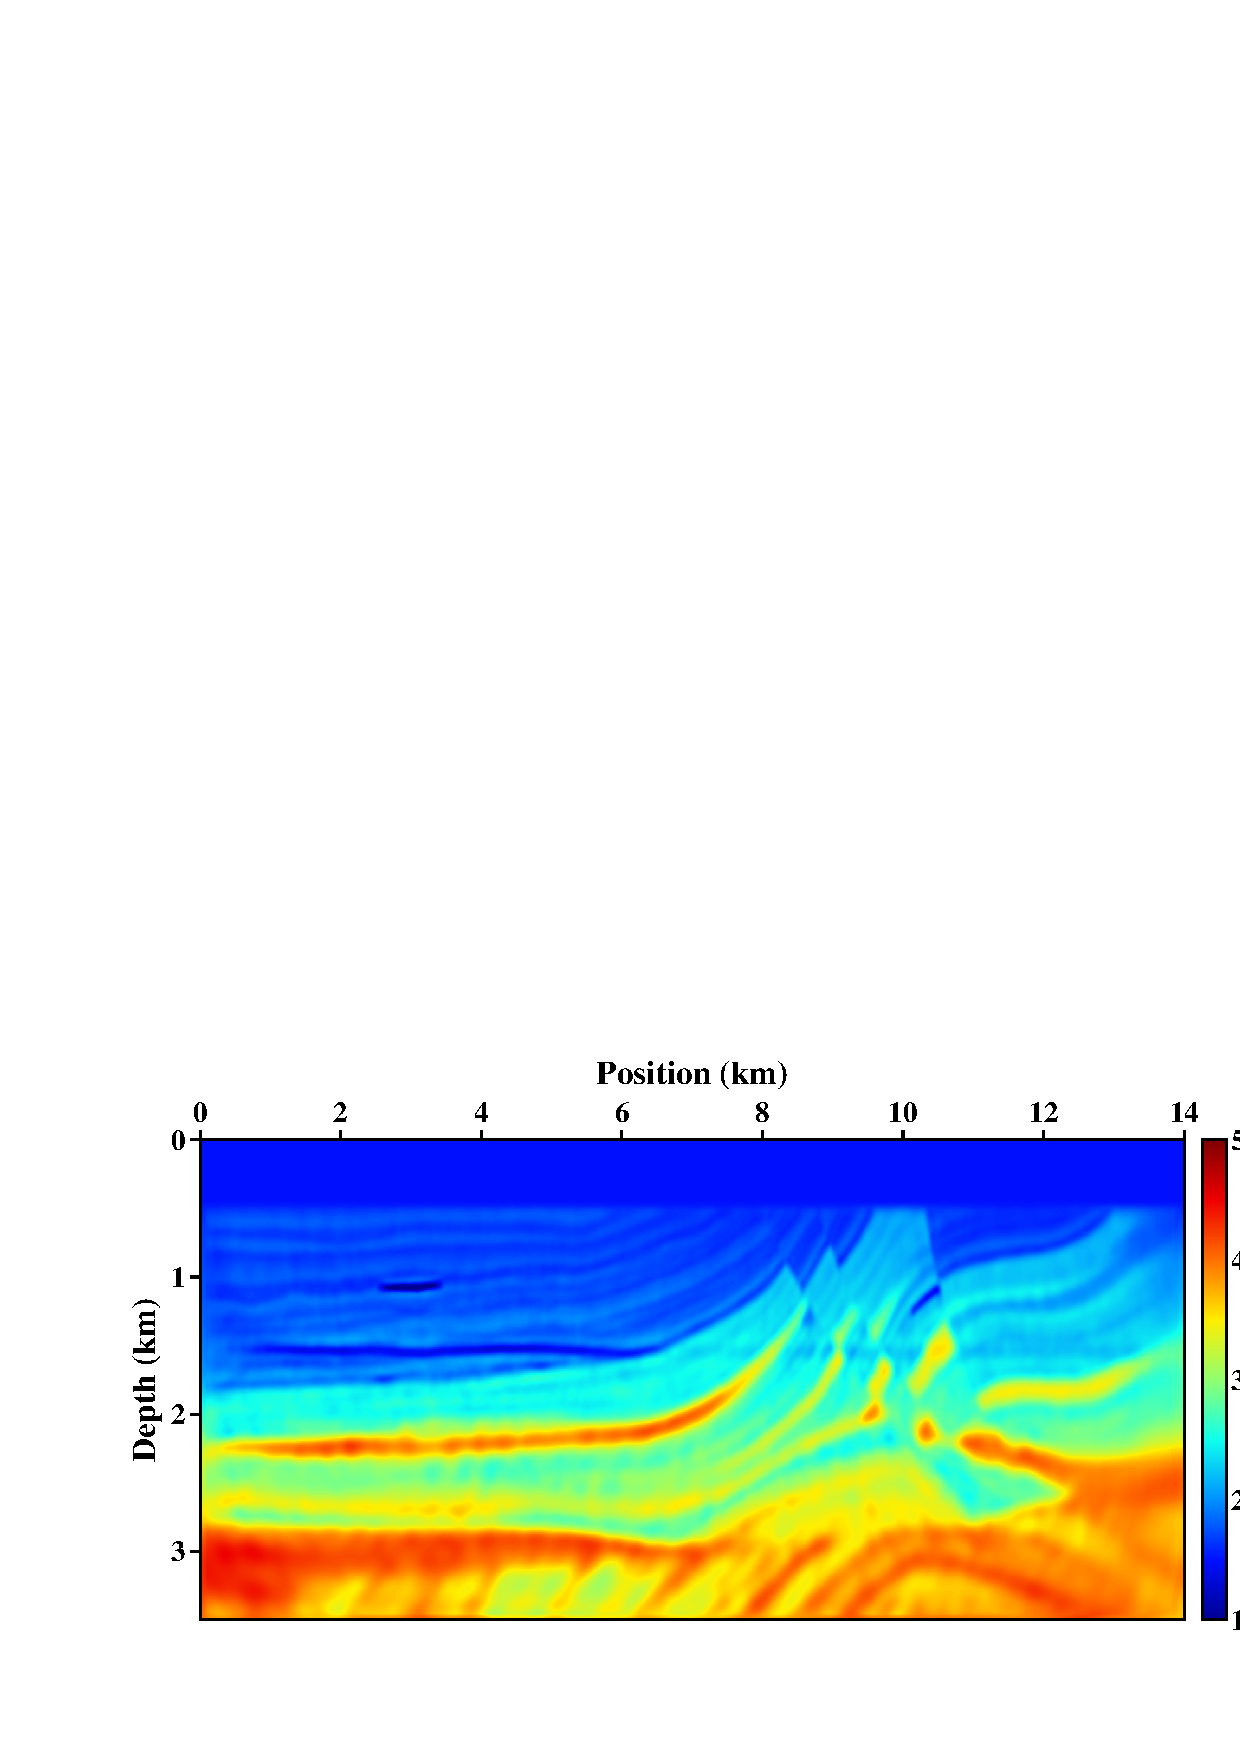
\includegraphics[width=7cm]{Figure/chapter02/tariqsugresult/Fig/1nodevp.pdf}}
        \subfloat[]{\includegraphics[width=7cm]{Figure/chapter02/tariqsugresult/Fig/1devp.pdf}}\\
        \subfloat[]{\includegraphics[width=7cm]{Figure/chapter02/tariqsugresult/Fig/1nodevs.pdf}}
        \subfloat[]{\includegraphics[width=7cm]{Figure/chapter02/tariqsugresult/Fig/1devs.pdf}}\\
        \subfloat[]{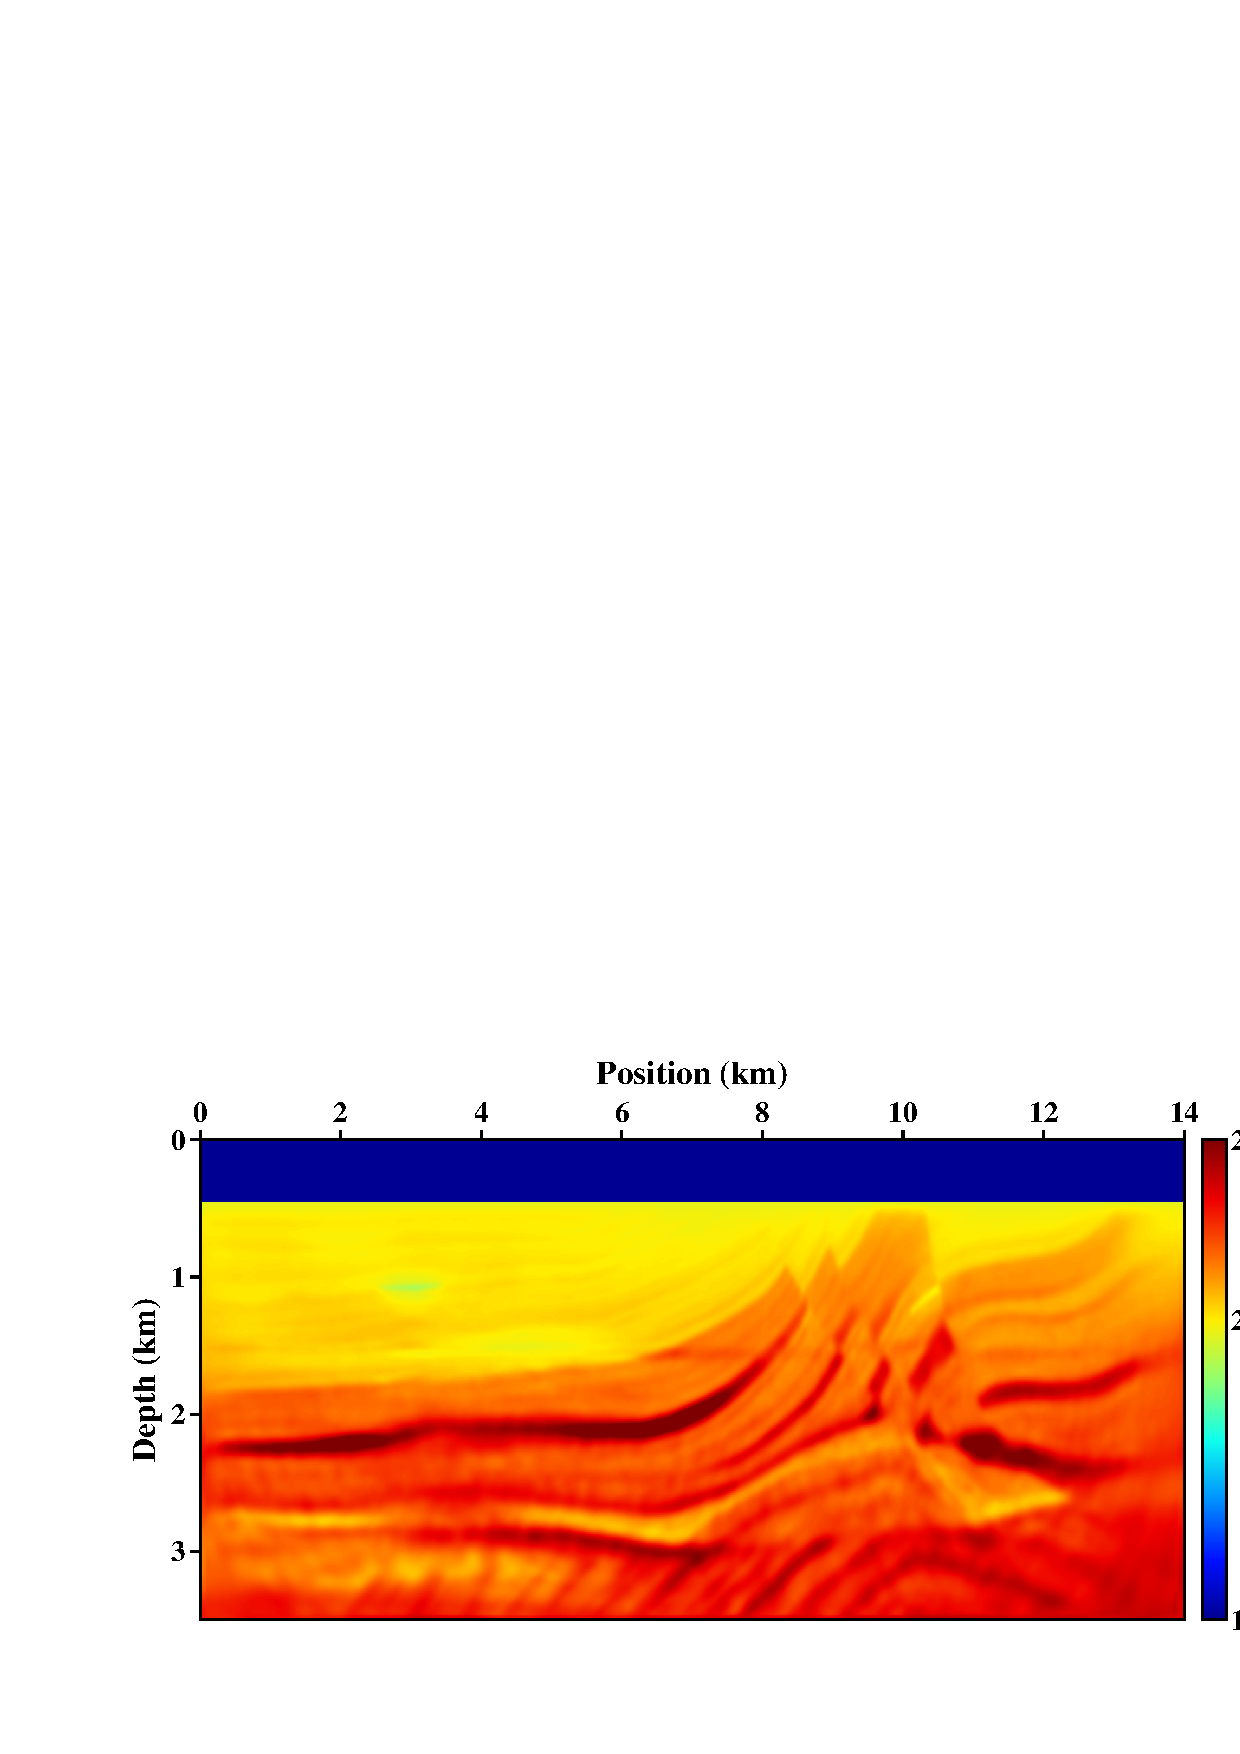
\includegraphics[width=7cm]{Figure/chapter02/tariqsugresult/Fig/1noderho.pdf}}
        \subfloat[]{\includegraphics[width=7cm]{Figure/chapter02/tariqsugresult/Fig/1derho.pdf}}
        \caption{
			密度变化时常规和模式解耦的EFWI结果对比。左侧为常规PCG方法反演结果,右侧为MDPCG方法反演结果。
			其中(a),(b)为$V_p$; (c), (d)为$V_s$; (e), (f)为$\rho$。
%			Comparison between conventional and MD-based method with density
%            variation: (a) - (c) are the inverted $V_p$, $V_s$ and $\rho$ with
%            conventional method, (d) - (f) are the inverted $V_p$, $V_s$ and $\rho$
%            with MD-based method. 
		}
    \label{fig:InvertWithRho}
    \end{center}
\end{figure*} 
\begin{figure*}
    \begin{center}
        {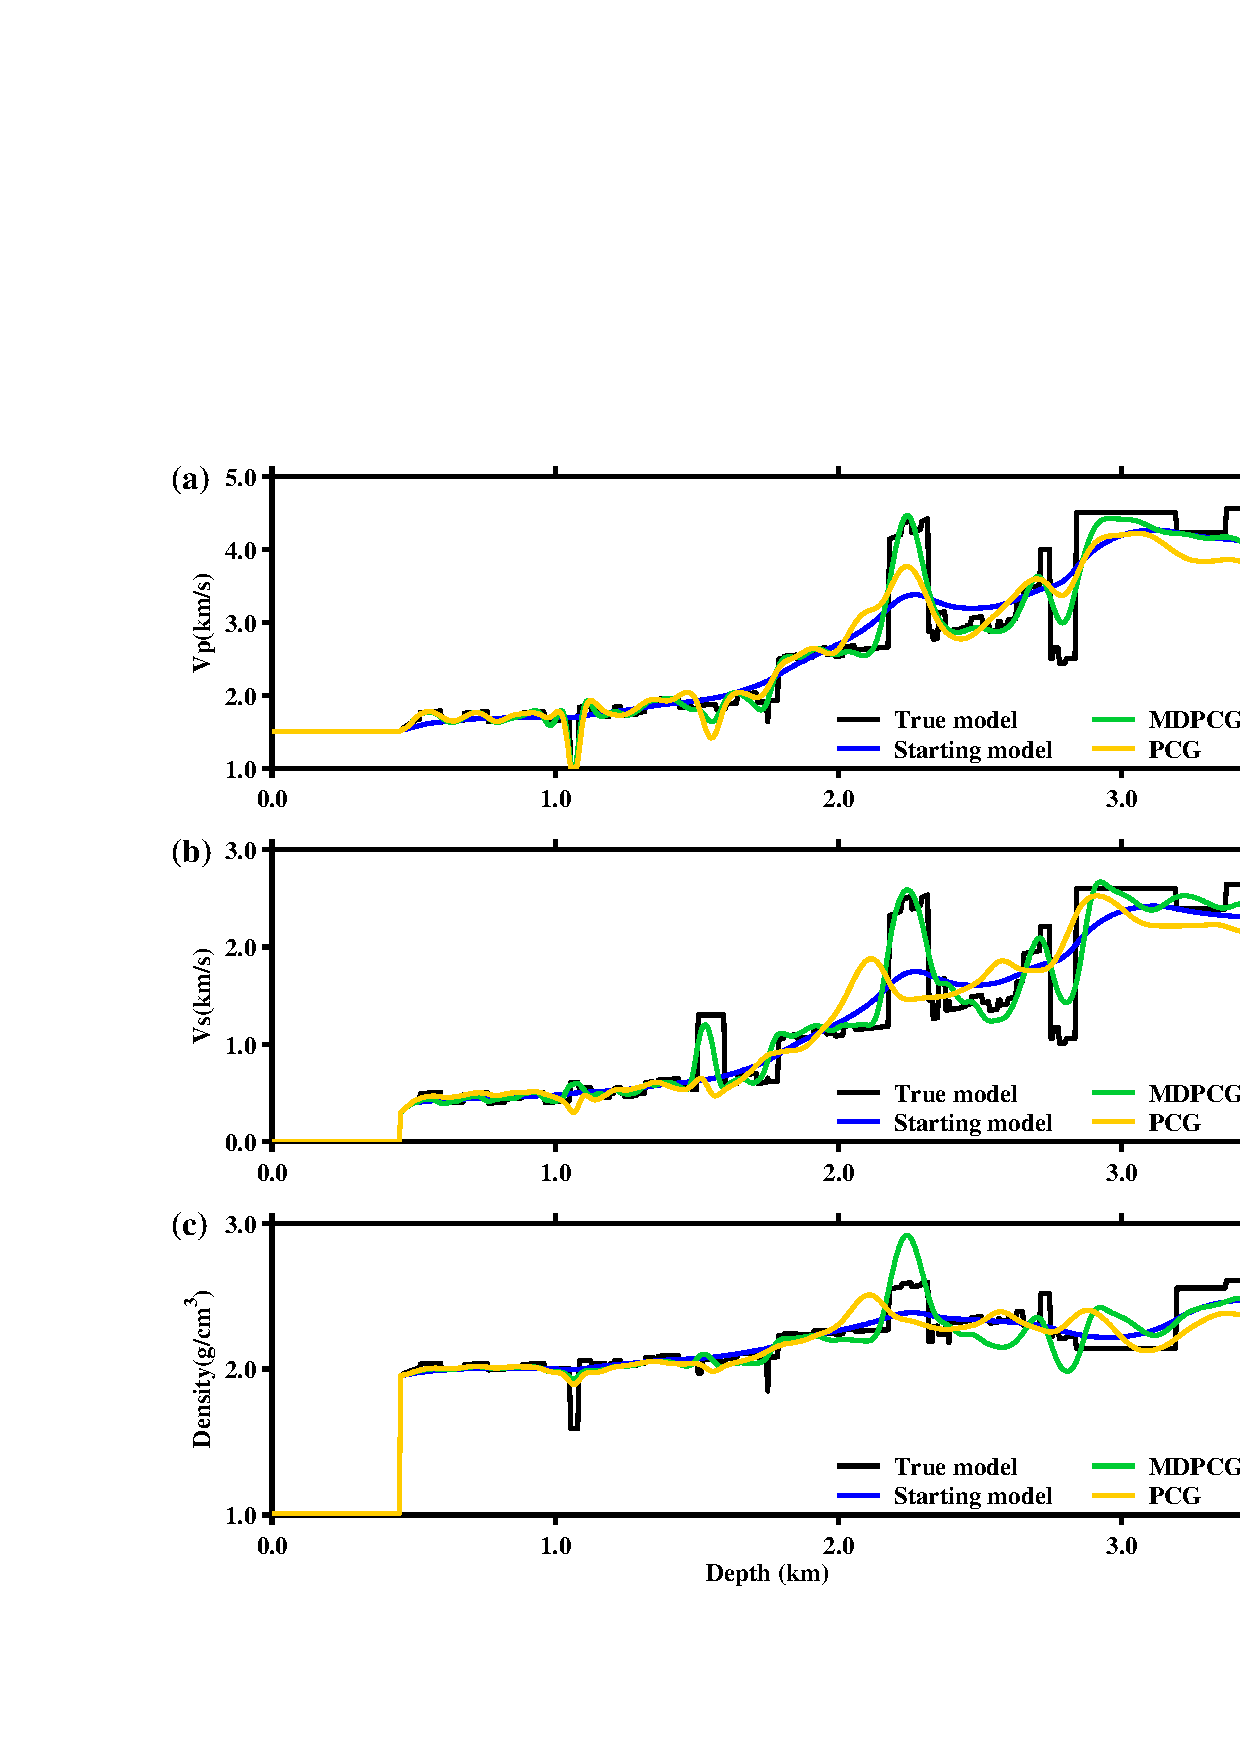
\includegraphics[width=10cm]{Figure/chapter02/tariqsugresult/Fig/3kmrho.pdf}}
        \caption{
			速度与密度模型在3.0km处的纵向剖面。
			黑线和蓝线分别代表真实和初始模型;黄线与绿线分别代表常规PCG和MDPCG方法反演结果。
%        The velocity and density profiles at 3.0 km (a, b)  with the true models
%            (black),
%            the initial models (blue), the PCG-based (yellow) and MD-based (green)
%            inverted models.
    }
    \label{fig:RhoProfile3km}
    \end{center}
\end{figure*}
\begin{figure*}
    \begin{center}
        {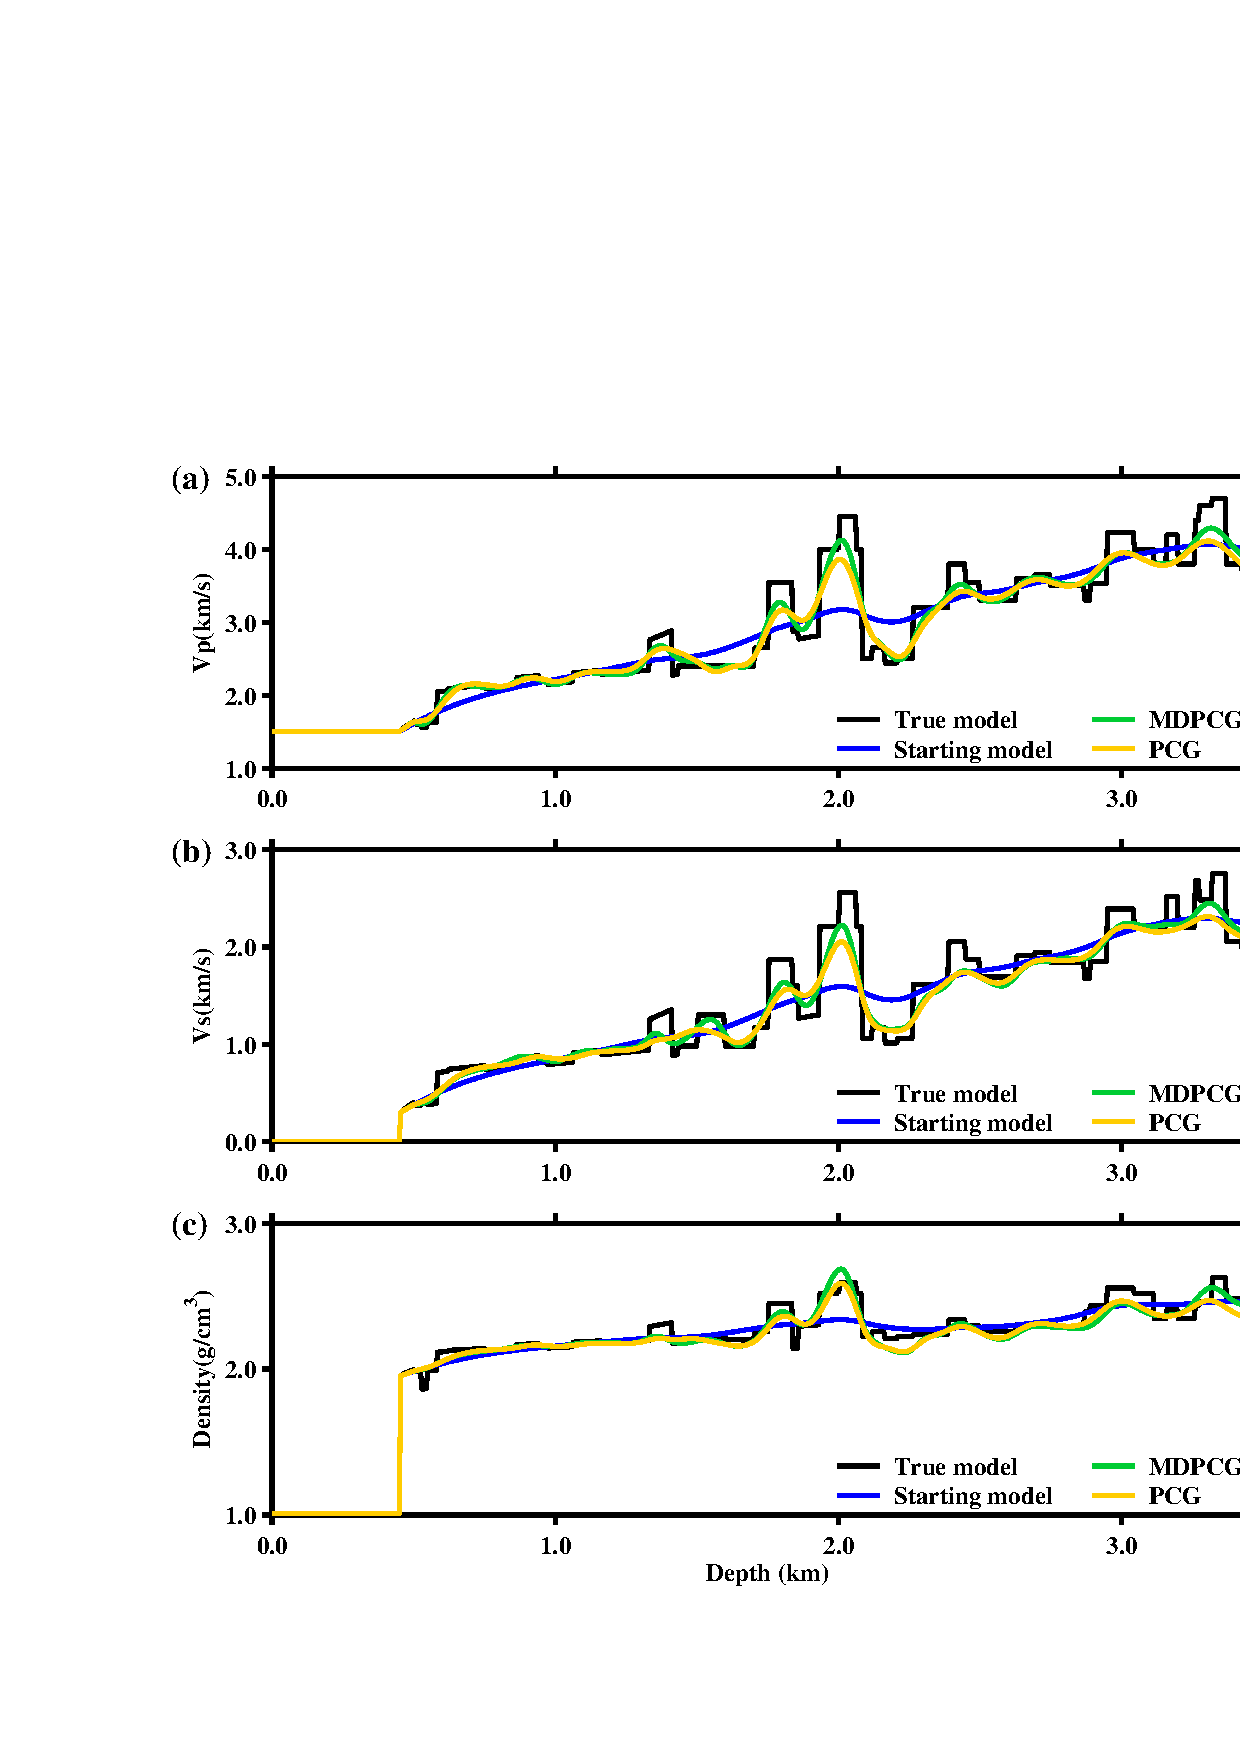
\includegraphics[width=10cm]{Figure/chapter02/tariqsugresult/Fig/9kmrho.pdf}}
        \caption{
			速度与密度模型在9.0km处的纵向剖面。
			黑线和蓝线分别代表真实和初始模型;黄线与绿线分别代表常规PCG和MDPCG方法反演结果。
%        The velocity and density profiles at 9.0 km (a, b)  with the true models
%            (black),
%            the initial models (blue), the PCG-based (yellow) and MD-based (green)
%            inverted models.
    }
    \label{fig:RhoProfile9km}
    \end{center}
\end{figure*} 

\section{本章小结}
多参数耦合效应使得常规梯度类EFWI受到很大挑战,即使是只考虑P和S波速度的反演。辐射模式表明两种速度扰动都会产生P波数据扰动从而导致在特定散射角范围内的
重叠效应。相反,S波扰动波场则只与S波速度扰动相关。通过引入弹性波模式解耦,本文发现在解耦之后,不同波模式的Frech{$\acute{e}$}t和数据残差之间的互相关对梯度
的贡献非常微弱。通过该交叉项近似,导出了基于模式解耦的梯度,该梯度可以通过伴随状态法快速计算得到。利用解耦之后的Frech{$\acute{e}$}t导数,调查了
Hessian以及分辨率矩阵对应于P波与S波数据的有关分量。这些调查确认了在S波速度的梯度计算中丢弃P波分量可以降低参数耦合效应。因此,采用基于模式解耦的方法
来反演$V_s$等价于采用S波数据的单参数反演。借助较好的预条件算子消除S波数据的照明以及有限带宽效应,就能获得近似GN方法的收敛速度而不涉及
任何Hessian相关的计算。对于双参数同时反演,$V_s$反演的改善可以明显提高$V_p$的反演精度。数值实验尤其是包含软海底结构的Marmousi模型实验,表明模式解耦方法
对压制参数耦合、加速收敛是有效的。

到目前为止,通过波形反演来重建可靠的密度模型仍然非常困难。正如我们所看到的那样,模式解耦并未改善密度反演结果。但是在引入密度扰动后,反演病态性明显加剧后,采用MDPCG方法的EFWI仍能保证
获得比较合理的$V_p$和$V_s$结果。

%\chapter{弹性波波动方程反射走时反演}

\section{引言}
%尽管常规FWI在长偏移距,宽方位数据中有着令人满意的效果,但是在这种观测系统下,
目前FWI应用成功的案例中,主要利用了长偏移距透射波以及临界反射波等来更新速度模型的
中低波数分量。中深部的模型更新则主要集中在偏移响应对应的高波数部分。
在中深部区域,即使以目前大偏移距、宽方位的观测技术也难以保证有足够的透射波穿过。
如何利用现有数据准确反演中深部速度模型的中低波数成分是人们非常关心的课题。

反射波可以更好地照明深部结构。
受MBTT方法的启发,Xu et al
(2012)\cite{xu:2012}提出了反射波波形反演方法(RWI),
通过反射波来产生类似透射路径的信息来获得中低波数成分的更新。
RWI基于波动理论建立中深部背景模型的思路立即获得了广泛的关注(Wang et al., 2013\cite{Wang2013}; Wu and Alkhalifah, 2015; 
Zhou et al., 2015\cite{zhou:2015}; Guo and Alkhalifah, 2016\cite{Guo2016})。
它实质是通过最小平方偏移等手段获取“真振幅”的反射率,然后利用反偏移预测出反射波数据,并将它与观测数据的波形残差
反投影到Born波路径上进行背景速度更新。
%近期,Irabor and
%Warner(2016)\cite{Irabor2016}和Wang et
%al(2016)\cite{WangFangEtAl2016}在初始模型中加入高频扰动并通过上下形波分离来获取常规FWI中能够更新背景速度的梯度分量,实质上也利用了反射波波路径的信息。
%然而波形匹配并非是RWI中最合适的拟合方式。
尽管RWI的目的在于更新背景速度,
当初始模型偏离真值较远时,反射波波形匹配也会受到cycle-skipping影响。这时分频等多尺度策略会有助于避免cycle-skipping现象\cite{Wang2013}。此外,利用
走时信息构建目标函数也可以较好地避免上述问题。

在成像域利用反射波更新背景速度的方法由来已久,如射线层析\cite{Stork1992}。波动方程速度偏移分析(WEMVA)近年来也获得了长足的发展(
Sava and
Fomel(2006)\cite{SavaEtAl2006}; Yang and Sava(2011)\cite{YangEtAl2011}; Almomin and
Biondi(2012)\cite{Almomin2012}; Sun and Symes(2012)\cite{SunEtAl2012})。
WEMVA通常需要引入扩展成像条件,采用各类准则衡量成像残差,例如叠加能量最大(SI)\cite{ChaventEtAl1995}、微分相似优化(DSO)\cite{SymesEtAl1991}
和差异剩余偏移(DRM)\cite{SavaEtAl2004}等来实现背景模型的更新。
但WEMVA受困于昂贵的计算代价,尤其在三维问题中。
%针对反射走时,Luo et
%al(2016)\cite{Luo2016}用时间轴方向的扩展成像与Rytov近似结合,导出了全走时反演(FTI)方法,获得了不错的反演效果。该方法实质上也是一种成像域的反演方法。

为了克服振幅拟合有关的目标函数带来的非线性,本章采用与背景速度更加线性相关的
走时信息来构建目标函数。通过动态图像识别(DIW)技术来获取模拟与观测反射数据之间的时移量\cite{ma2013},提出了弹性波波动方程反射走时反演(EWERTI)方法。
相比互相关提取时移(空移)量的方式\cite{chi2015,Wang2015},DIW能更准确地获取局部的走时差异。
%Ma and
%Hale(2013)\cite{ma2013}采用动态图像识别(DIW)来获得模拟与观测反射数据之间的时移,从而导出了波动方程反射走时反演(WERTI)。Chi
%et al (2015)\cite{chi2015}和Wang et al
%(2015)\cite{Wang2015}采用互相关类的方法来获取时移(或空移)。
此外,弹性波走时反演中需要处理模式转换产生的虚假反射波路径的问题,即
需要根据对应的PP波与PS波波路径(假设P波震源)更新$V_p$与$V_s$模型。
文中将联合地面P/S分离+DIW获取不同波模式的走时残差,并通过空间波场模式解耦预条件梯度来降低非线性程度、压制参数耦合等。
在此基础上,设计出两步的反演流程来实现稳健的EWERTI方法。Sigsbee2A模型的数值实验将验证EWERTI方法的有效性。
%但尽管如此,RWI中的强非线性问题仍然存在,尤其是在使用波形匹配的目标函数时。
%虽然波形信息能提高反演精度,但是走时信息对模型的低波数成分扰动更敏感,二者之间具有更好的线性关系。
%因此我们使用走时残差的$L_2$范数
%作为目标函数,而走时信息则采用DIW获取。
%由于PP与PS走分别包含在在P波与S波地震记录中,因此还需要采用地面数据分离的方式
%分解出P或S波数据,才能保证准确获取PP和PS波走时信息。%本章中采用EWERTI的方式,通过两步法的策略建立$V_p$与$V_s$的背景模型。
%所以,采用走时反演来为常规FWI建立合适的含有长波长信息的初始
%%模型会更加稳健有效\cite[]{Ma2013, Chi2015, Luo2016}。然而在弹性介质中,这中思路会受到限制,
%因为弹性波场中存在复杂的模式转换,这就导致很难获得单一波模式的走时
%信息。
\section{弹性波波动方程反射走时反演}
利用拟合反射波来反演模型参数就需要预测出反射波数据,再与观测数据进行匹配。
弹性反射波的模拟通常采用偏移/反偏移的方式实现。
在EWERTI中,需要匹配反射波数据的走时信息,
并将走时残差反投影到反射波路径上更新背景速度模型。下面从弹性波方程出发导出EWERTI的梯度公式。
反演过程中,
同样假设在背景弹性介质($c_{ijkl}$)中有参数扰动$\delta c_{ijkl}$,则背景波场与扰动波场分别满足以下方程:
\begin{equation}
    \rho \frac{\partial u^2_i}{\partial t^2}  -
    \frac{\partial}{\partial x_j}\left[ 
        c_{ijkl}\frac{\partial u_{k}}{\partial
        x_l}\right]=f_i,
    \label{eq:WE_3} 
\end{equation}
和
\begin{equation}
    \rho \frac{\partial \delta u^2_i}{\partial t^2}  -
    \frac{\partial}{\partial x_j}\left[ 
        c_{ijkl}\frac{\partial \delta u_{k}}{\partial
        x_l}\right]=\frac{\partial}{\partial x_j}\left[\delta c_{ijkl}\frac{\partial u_{k}}{\partial x_l}\right],
    \label{eq:DeltaWE} 
\end{equation}
这里$\delta u_i$可以看作是用ERTM或其他方法获得的成像结果($\delta c_{ijkl}$)进行反偏移构建的反射波数据。
观测数据$\mathbf{d}^{o}$与模拟数据$\mathbf{d}^{c}$之间的走时残差需要达到最小,则目标函数写成:
\begin{equation}
	\left\{
		\begin{aligned}
			&\tau(\mathbf{x_r},t;\mathbf{x_s})=\mathop{\arg\min}_{\tau}
			\parallel\mathbf{d}^{c}(\mathbf{x}_r,t;\mathbf{x}_s)-\mathbf{d}^{o}(\mathbf{x}_r,t+\tau;\mathbf{x}_s)\parallel^2\\
    &E=\frac{1}{2}\int\tau^2(\mathbf{x_r},t;\mathbf{x_s})dtd\mathbf{x_r}d\mathbf{x_s},
		\end{aligned}
	\right.
    \label{eq:Objectivefunction} 
\end{equation}
其中走时残差$\tau(\mathbf{x_r},t;\mathbf{x_s})$可以通过DIW技术来获取。通过类似Ma and
Hale (2013)\cite{ma2013}的推导(见附录\ref{cha:AdjointForEWERTI}),本文导出了如下梯度公式:
\begin{equation}
    \frac{\partial E}{\partial c_{ijkl}}=-\int (\frac{\partial u_{i}}{\partial
    x_j}\frac{\partial \delta \psi_{k}}{\partial x_l}+\frac{\partial \delta u_{i}}{\partial
    x_j}\frac{\partial \psi_{k}}{\partial x_l}),
    \label{eq:GradientCijkl}
\end{equation}
其中,$\psi_i$和$\delta \psi_i$是共轭的背景波场和散射波场,满足:
\begin{equation}
    \rho \frac{\partial \psi^2_i}{\partial t^2}  -
    \frac{\partial}{\partial x_j}\left[ 
        c_{ijkl}\frac{\partial \psi_{k}}{\partial
        x_l}\right]=\tau(\mathbf{x_r},t;\mathbf{x_s})\frac{\dot{d}^o_i(\mathbf{x_r},t+\tau;\mathbf{x_s})}{h_i(\mathbf{x_r},t;\mathbf{x_s})},
    \label{eq:AdjointWE} 
\end{equation}
和
\begin{equation}
    \rho \frac{\partial \delta \psi^2_i}{\partial t^2}  -
    \frac{\partial}{\partial x_j}\left[ 
        c_{ijkl}\frac{\partial \delta \psi_{k}}{\partial 
        x_l}\right]=\frac{\partial}{\partial x_j}\left[\delta c_{ijkl}\frac{\partial
        \psi_{k}}{\partial x_l}\right], 
    \label{eq:AdjointDeltaWE} 
\end{equation}
式中$h_i(\mathbf{x_r},t;\mathbf{x_s})=(\dot{d}^o_i(\mathbf{x_r},t+\tau;\mathbf{x_s}))^2-\ddot{d}^o_i(\mathbf{x_r},t+\tau;\mathbf{x_s})
(d^c_i(\mathbf{x_r},t;\mathbf{x_s})-d^o_i(\mathbf{x_r},t+\tau;\mathbf{x_s}))$,而$\dot{d}$则代表$d$的时间导数。
需要注意的是,上式伴随源的分母中包含有地震记录的二阶导数,会导致除法的不稳定,这里采用时间方向的积分
$h^{'}_i(\mathbf{x_r};\mathbf{x_s})=\int h_i(\mathbf{x_r},t;\mathbf{x_s})dt$
来代替原有的分母项(付继有等,2015\cite{Fu2015})。
在方程\eqref{eq:GradientCijkl}的右端
,第一和第二项分别表示震源端和检波点端的反射波路径。可以通过链式法则导出P波与S波速度的梯度公式:
\begin{equation}
\begin{split}
    &\frac{\partial E}{\partial V_p}=2\rho V_p\frac{\partial E}{\partial
        c_{ijkl}}\delta_{ij}\delta_{kl}, \\
    &\frac{\partial E}{\partial V_s}=2\rho V_s\frac{\partial
    E}{\partial c_{ijkl}}(-2\delta_{ij}\delta_{kl}+\delta_{ik}\delta_{jl}+
    \delta_{il}\delta_{jk}).
\end{split}
    \label{eq:GradientVel}
\end{equation}

\section{弹性波反射波路径核函数}
反射波反演的关键是将预测的与观测的反射波之间的残差反投影到反射波路径上,从而实现对模型的更新。因此,反射波波路径的计算将是反演中
的核心任务。由于弹性波中存在各种模式转换,所以反射波波路径的复杂程度远大于声波中的情况。首先分析弹性波反射波路径的性态,并尝试通过
模式解耦克服反演中遇到的部分困难。
由附录\ref{cha:AdjointForEWERTI}推导可看出,不同的目标函数只影响共轭状态方程的伴随震源项,并不影响最终梯度的互相关方式。
因此分析弹性反射波波路径的核函数性态将有助于理解模式耦合引起的问题,从而为压制梯度中的假象并帮助设计新的反演策略提供理论依据。
\begin{figure}[!htb]
   \centering
   \subfloat[]{\includegraphics[width=0.50\textwidth]{Figure/chapter03/Kernel/1vp.pdf}}
   \subfloat[]{\includegraphics[width=0.50\textwidth]{Figure/chapter03/Kernel/1vs.pdf}}\\
   \subfloat[]{\includegraphics[width=0.50\textwidth]{Figure/chapter03/Kernel/Vponlyvp.pdf}}
   \subfloat[]{\includegraphics[width=0.50\textwidth]{Figure/chapter03/Kernel/Vsonlyvp.pdf}}\\
   \caption{单$V_p$界面的反射波路径。(a) $V_p$模型,(b) $V_s$模型,(c) $V_p$敏感核函数,(d) 
   $V_s$敏感核函数.}
   \label{fig:kernel1_vp}
\end{figure}

为了简化表达,将式\eqref{eq:GradientCijkl}重新写作:
\begin{equation}
    \nabla E(
    \mathbf{m}_0)=-\int(
    \mathbf{u}\cdot\delta \boldsymbol{\psi}
    +\delta
    \mathbf{u}\cdot{\boldsymbol{\psi}})
    \label{eq:kernelgradient} 
\end{equation} 
其中$\mathbf{u}$和$\boldsymbol{\psi}$为背景介质的正传与共轭波场,$\delta\mathbf{u}$和$\delta \boldsymbol{\psi}$为正传与共轭的散射场。
这里统一用$\cdot$表示波场分量的互相关。上式只示意性表达出反射波路径的计算方式,而不同参数化方式相应的具体计算公式需要参照链式法则获得。
上式中第一项表示震源到反射界面的波路径,第二项表示从反射界面到检波点的波路径。考虑到
波场解耦,上式的梯度也可以分解成P或S波数据组合的分量:
\begin{equation}
    K_m^{MN}     
    =-\int(\mathbf{u}^M\cdot\delta \boldsymbol{\psi}^N
    +\delta  \mathbf{u}^M\cdot\boldsymbol{\psi}^N),\\
    \label{eq:decompkernel} 
\end{equation}
其中$m\in\{V_p, V_s\}$,$M,N\in\{P,S\}$。

为了观察弹性波反射波路径(敏感核函数),先在单界面模型中计算反射波波路径。假定只有$V_p$的扰动界面(如图\ref{fig:kernel1_vp}a和b)。
%\begin{figure}
%   \centering
%   \subfloat[]{\includegraphics[width=0.38\textwidth]{Figure/chapter03/Kernel/1vp.pdf}}
%   \subfloat[]{\includegraphics[width=0.38\textwidth]{Figure/chapter03/Kernel/1vs.pdf}}\\
%   \caption{单独$V_p$扰动界面。左侧为$V_p$,右侧为$V_s$.}
%   \label{fig:KernelModel1}
%\end{figure}
由于没有$V_s$扰动,因此没有模式转换能量而只有PP波反射,非常接近于声波情况。
采用该模型获得的反射波波路径如图\ref{fig:kernel1_vp}c和d。可以看到,$V_p$的反射波
路径分为震源端以及检波点端左右两支,与声波波路径非常接近。同时,$V_s$也会有相应的波路径能量,但是主要集中在边缘部分,第一菲涅尔带中央区域
能量较弱。原因可能是这部分波路径信息是与PP波反射能量对应的,对$V_s$背景信息并不敏感。
%如果换做$\lambda$和$\mu$的参数化方式,其产生的波路径如图\ref{Kernel1_lambda}所示
%\begin{figure}
%   \centering
%   \subfloat[]{\includegraphics[width=0.30\textwidth]{Figure/chapter03/Kernel/lambdaonlyvp.pdf}}
%   \subfloat[]{\includegraphics[width=0.30\textwidth]{Figure/chapter03/Kernel/muonlyvp.pdf}}\\
%   \caption{图\ref{fig:KernelModel1}模型$\lambda$参数化时的反射波路径。左侧为$\lambda$,右侧为$\mu$.}
%   \label{fig:kernel1_lambda}
%\end{figure}
\begin{figure}[!htb]
   \centering
   \subfloat[]{\includegraphics[width=0.50\textwidth]{Figure/chapter03/Kernel/2vp.pdf}}
   \subfloat[]{\includegraphics[width=0.50\textwidth]{Figure/chapter03/Kernel/2vs.pdf}}\\
   \subfloat[]{\includegraphics[width=0.50\textwidth]{Figure/chapter03/Kernel/Vponlyvs.pdf}}
   \subfloat[]{\includegraphics[width=0.50\textwidth]{Figure/chapter03/Kernel/Vsonlyvs.pdf}}\\
   \caption{单$V_s$界面的反射波路径。(a) $V_p$模型,(b) $V_s$模型,(c) $V_p$敏感核函数,(d) 
   $V_s$敏感核函数.}
%   \caption{单独$V_p$扰动界面。左侧为$V_p$,右侧为$V_s$.}
   \label{fig:kernel2}
\end{figure}

然后,考虑$V_s$模型存在界面的情况(图\ref{fig:kernel2}a和b)。此时波场就会变得十分复杂
,在正传及反传波场中会同时存在P波与S波,导致反射波路径变得更加复杂。
%\begin{figure}
%   \centering
%   \subfloat[]{\includegraphics[width=0.30\textwidth]{Figure/chapter03/Kernel/Vponlyvs.pdf}}
%   \subfloat[]{\includegraphics[width=0.30\textwidth]{Figure/chapter03/Kernel/Vsonlyvs.pdf}}\\
%   \caption{单独$V_p$扰动时的反射波路径。左侧为$V_p$,右侧为$V_s$.}
%   \label{fig:kernel2}
%\end{figure}
\begin{figure}[!htb]
   \centering
   \subfloat[]{\includegraphics[width=0.50\textwidth]{Figure/chapter03/Kernel/VsonlyvsPP.pdf}}
   \subfloat[]{\includegraphics[width=0.50\textwidth]{Figure/chapter03/Kernel/VsonlyvsPS.pdf}}\\
   \subfloat[]{\includegraphics[width=0.50\textwidth]{Figure/chapter03/Kernel/VsonlyvsSP.pdf}}
   \subfloat[]{\includegraphics[width=0.50\textwidth]{Figure/chapter03/Kernel/VsonlyvsSS.pdf}}
   \caption{$K_{V_s}$敏感核函数的四个分量:(a) $K_{V_s}^{PP}$, (b) $K_{V_s}^{PS}$, (c) $K_{V_s}^{SP}$, (d) $K_{V_s}^{SS}$.}
   \label{fig:kernel2_vs_decomp}
\end{figure}
图\ref{fig:kernel2}中$V_p$敏感核函数与图\ref{fig:kernel1_vp}有所不同,这是因为当存在$V_s$反射界面时,反传的散射波场在界面处产生“非物理”的SP转换波,
这部分波场与背景场中的P波互相关就会产生一些假象。而在$V_s$的敏感核函数中,可以看到多种模式转换导致的多个波路径叠加,使得核函数十分复杂。
但是可以观察到其中的P波路径的能量总是占主导地位。
如果直接采用该核函数来计算目标函数关于$V_s$的梯度,一定会因为这些严重的cross-talk对反演带来更多的麻烦。

根据公式\eqref{eq:decompkernel},将原始的$V_s$核函数分解为四个部分。
如图\ref{fig:kernel2_vs_decomp}所示,$K_{V_s}^{PP}$与图\ref{fig:kernel2}c中
的$V_p$核函数十分类似,但是主要能量的符号相反(在第二章图\ref{fig:all}中有类似现象);$K_{V_s}^{PS}$与$K_{V_s}^{SP}$则包含非常多的高频信息,
它们主要是不同模式的正传与反传波场之间的偏移脉冲响应;$K_{V_s}^{SS}$则与其他三者有些不同,只包含了检波点端的单支反射路径,这是由于
采用了P波震源,在震源端的波场中不包含S波数据($K_{V_s}^{SS}$的震源端项会是0)。这样的话,$K_{V_s}^{SS}$就几乎不受到P波路径的影响。
如果利用这些后核函数分量的这些特征,
将会非常有助于背景$V_s$的反演。
\section{反射走时反演流程}
弹性介质中P波震源情况下,不同模式的转换波(主要是PP与PS波)同相轴之间会互相叠加、互相交叉。在用DIW提取走时残差的时候,这些交叉点的位置就会变成一些奇异点带来很大麻烦
。因此,如果直接用原始多分量数据的话,拾取到的$\tau(\mathbf{x_r},t;\mathbf{x_s})$就会不准确,这也是为什么式\eqref{eq:AdjointDeltaWE}中的梯度很难直接应用。
为了解决这个问题,本文将观测与模拟地震数据分解为P波与S波两部分。该模式分解只作用于地面地震数据\cite[]{Li2016a},可以快速地获得每一炮数据分解之后的矢量
P波或S波地震记录。这样,走时残差就可以被分成P波与S波两部分,使得弹性波WERTI变得可行。于是,设计出一个两阶段的反演流程,先P波阶段后S波阶段。
由于DIW提取走时的方式对数据的频率成分并不敏感,因此EWERTI中的多尺度策略主要体现在参数反演先后顺序上,并不需要过多考虑分频的策略。

$\quad$

$\quad$

$\quad$
\subsection{$V_p$反演}
在这个阶段主要采用PP反射波来建立P波速度的背景模型。首先,从ERTM中获得P波速度的扰动,即$\delta V_p$。
因为在速度不准的情况下大偏移距数据的偏移/反偏移结果会
造成模拟的反射波零偏移距走时误差,进而增加反演的非线性程度。
这里为了确保模拟数据与观测数据中零(小)偏移距反射走时相匹配,只采用小偏移距的数据
获取$\delta V_p$。
此外,由于在EWERTI中只考虑走时,可以只进行ERTM成像
而不是ELSRTM来估计反射率。
这也降低了反演中对反射系数估计的依赖程度。因此,目标函数变为最小化PP反射波的走时残差:
\begin{equation}
    E_{pp}=\frac{1}{2}\int\tau^2_{pp}(\mathbf{x_r},t;\mathbf{x_s})dtd\mathbf{x_r}d\mathbf{x_s}.
    \label{eq:ObjectivefunctionPP} 
\end{equation}
这样,采用分离的P波记录来计算方程\eqref{eq:AdjointWE}的右端项,并用$\delta V_p$替换方程\eqref{eq:DeltaWE}和\eqref{eq:AdjointDeltaWE}中的$\delta c_{ijkl}$,
就可以计算得到$V_p$的梯度($\frac{\partial E}{\partial V_p}$)。与EFWI一样,该梯度中的互相关项自动隐含了散度算子。因此,在
计算时只利用了PP反射波,所以不需要额外施加空间域的模式解耦。这个PP波走时反演本质上接近于声波反射走时反演,区别在于需要将地
面多分量地震记录进行数据域模式分离。注意,在分离后的数据中可能包含部分SP模式的转换波,它们对$V_p$的反演可能造成不利的影响,这需要今后更深入的研究。

\subsection{$V_s$反演}
接下来将对PS反射波采用类似的反演。相应地,目标函数变为:
\begin{equation}
    E_{ps}=\frac{1}{2}\int\tau^2_{ps}(\mathbf{x_r},t;\mathbf{x_s})dtd\mathbf{x_r}d\mathbf{x_s}.
    \label{eq:ObjectivefunctionPS} 
\end{equation}
值得一提的是,PS反射波的模拟(预测)方式与前一阶段略有不同。这里有两种方式来模拟PS反射波:

方式\uppercase\expandafter{\romannumeral1}: 采用反演好的$V_p$以及初始$V_s$模型来实现PS波偏移成像,然后使用该成像结果进行反偏移;

方式\uppercase\expandafter{\romannumeral2}: 由于$V_p$的背景速度在前一阶段已经被较好地恢复,此时PP波成像结果应该比较接近准确位置。考虑到大多数情况下,地
下介质中$V_p$与$V_s$的界面是比较一致的,因此也可以采用PP波成像结果作为界面来模拟PS反射波。

经过测试,发现第一种方式产生的近偏移距走时
对$V_p$模型的误差非常敏感,即使$V_p$模型在真值附近扰动也有可能获得方向错误的走时残差。
对于非对称的PS反射波的路径,假定地下存在如图\ref{fig:PS_refl}所示的单界面PS波反射。
由几何关系以及Snell定律,存在如下关系
%入射角$\theta_1$与反射角$\theta_2$之间以及深度、偏移距与该角度之间的关系为:
\begin{equation}
%\begin{split}
    \frac{sin\theta_1}{V_p}=\frac{sin\theta_2}{V_s},\qquad
    h(tan\theta_1+tan\theta_2)=X,
%\end{split}
    \label{eq:Snell_PS} 
\end{equation}
\begin{figure}
   \centering
   \subfloat{\includegraphics[width=0.40\textwidth]{Figure/chapter03/PS_problem/PS_refl.pdf}}
   \caption{单界面PS反射波示意图。}
   \label{fig:PS_refl}
\end{figure}
其中$\theta_1$和$\theta_2$分别为入射和反射角,$h$为界面深度,则PS波时距曲线关系为:
\begin{equation}
	t=\frac{h}{cos\theta_1V_p}+\frac{h}{cos\theta_2V_s}.
    \label{eq:TravelTime_PS} 
\end{equation}
方式\uppercase\expandafter{\romannumeral1}与方式\uppercase\expandafter{\romannumeral2}的差异在于速度不准时,确定界面深度的过程不同。
这里数值分析时使用零(小)偏移距的图偏移获得界面深度,然后带入到
式\eqref{eq:TravelTime_PS}中来近似获得错误速度下反偏移预测的反射数据时距关系。

方式\uppercase\expandafter{\romannumeral1}
中,在图偏移时零偏移距走时保持不变,则偏移后的深度位置满足:
\begin{equation}
	\frac{h_{1}}{V^{'}_p}+\frac{h_{1}}{V^{'}_s}=\frac{h}{V_p}+\frac{h}{V_s},
    \label{eq:Mapmigration_PS} 
\end{equation}
其中$V^{'}_p$和$V^{'}_s$为错误的偏移速度。可以求得图偏移的深度:
\begin{equation}
	{h_{1}}=\frac{V^{'}_s(V_p+V_s)}{V_s(V^{'}_p+V^{'}_s)}h.
    \label{eq:ZerooffMig_PS} 
\end{equation}
而采用方式\uppercase\expandafter{\romannumeral2}时,在$V_p$存在误差时图偏移求得界面的深度为:
\begin{equation}
	{h_{2}}=\frac{V^{'}_p}{V_p}h.
    \label{eq:ZerooffMig_PP} 
\end{equation}
通常情况下
$V_p>V_s$因此$\frac{V_p+V_s}{V^{'}_p+V^{'}_s}$中$V^{'}_p$的小偏差也会带来很大的影响,
因此PS波零(小)偏移距成像界面的深度会同时受到$V_p$与$V_s$速度误差的影响。
下文将使用式\eqref{eq:Snell_PS}-\eqref{eq:ZerooffMig_PP}测试反偏移重建的反射数据的时距关系对$V^{'}_p$和$h$的敏感性。

这里将以下几个参数固定为$V_p=2500m/s$, $V_s=1500m/s$, $V^{'}_s=1300m/s$, 而$V^{'}_p$选取$2450,
2500, 2550m/s$三个扰动值。
从图\ref{fig:Sens_vp}可以看到,采用方式\uppercase\expandafter{\romannumeral1}时获取的反射数据对$V_p$的误差非常敏感,
在$\pm50m/s$范围内就会引起反偏移数据的走时残差改变方向
。相反,如果采用方式\uppercase\expandafter{\romannumeral2},其走时残差方向都是正确的。
\begin{figure}[h]
   \centering
   \subfloat[]{\includegraphics[width=0.5\textwidth]{Figure/chapter03/PS_problem/h1000.pdf}}
   \subfloat[]{\includegraphics[width=0.5\textwidth]{Figure/chapter03/PS_problem/h500.pdf}}
   \caption{不同界面深度时方式\uppercase\expandafter{\romannumeral1}(黑色虚线)与
   方式\uppercase\expandafter{\romannumeral2}(蓝色虚线)反偏移获得PS波走时曲线
   与真实值(红色实线)之间的对比。数字1,2,3分别代表不同$V^{'}_p$速度的结果。(a) 界面深度$h=1000$; (b) 界面深度$h=500$.}
   \label{fig:Sens_vp}
\end{figure}

所以,本文采用较为准确的PP成像($\delta V_p$)结果
%而不
%是$\delta V_s$
来产生PS反射波。
但这样做也存在两个弊端:
第一、产生的PS反射无法保证振幅的准确性,幸运的是这并不会给DIW拾取走时残差带来大的
困扰;第二、来自深部的PS反射可能由于时差太大使得DIW拾取受到cycle-skipping困扰。
不过这个问题可以采用“层剥离”的方式,通过照明能量补偿的控制,先使用浅部的反射走时残差来更新浅层,
再使用深部的走时残差更新深部的速度。这样即使初始阶段深部的反射走时残差拾取错误也不影响浅部的速度更新。
在浅部更新较好后,深部的反射走时残差也能保证拾取得较为准确。
%先更新浅层$V_s$
%然后更新深层来避免。
%但方式\uppercase\expandafter{\romannumeral2}也存在问题,
%即在界面深度较深时,Born模拟的走时偏离真值较远,如果存在多个同相轴就会难以进行震相间的匹配,这样即使DIW也会受到
%cycle-skipping影响,但幸运的是界面深度较浅时,Born模拟走时与观测数据偏离并不远,这样的话可以层剥离的方式来从浅到深反演
%解决深层反射的震相匹配问题。

此外,正如前文核函数分析提到,PS反射中震源端波路径只与P波速度相关,
因此在计算$\frac{\partial E}{\partial V_s}$时可以丢掉方程\eqref{eq:GradientCijkl} 
右端项的第一部分。同时,波模式分解也会施加在梯度的计算过程中来确保只有S波能量参与计算,即:
\begin{equation}
    \frac{\partial E_{ps}}{\partial V_s}=-2\rho V_s
    \int (\frac{\partial \delta u^S_{i}}{\partial
    x_j}\frac{\partial \psi^S_{k}}{\partial x_l})
    (\delta_{ik}\delta_{jl}+
    \delta_{il}\delta_{jk}).
    \label{eq:GradientVel_S}
\end{equation}
该模式解耦的梯度与Wang et al.
(2015)\cite{wang:2015}提出的EFWI预条件方式类似,可以在$V_s$的反演中降低参数耦合的影响

\section{局部倾角导引正则化}
数据域的WERTI与成像域射线走时层析有一些相似特性。通常,射线走时层析由于射线路径覆盖不均匀、反射界面深度与速度之间存在耦合等问题会导致反演的多解性,
所以射线层析通常不收敛或者很难收敛到正确的速度模型。
常规各向同性平滑算子的正则化约束可以一定程度上降低上述多解性的困扰,但是也很难保证反演收敛到具有地质含义的物理模型。
在偏移后,成像结果可以提供地下界面大致的倾角信息,由此设计正则化算子来沿地层倾角对反演进行约束可以
有效地应对多解性的问题,从而加快收敛速度、改善反演结果。由于采用波动方程作为波场传播引擎,WERTI采用波路径信息来反投影走时残差,因而所面临的多解性挑战要
小于射线走时层析。不过,对于一些照明不足或者
反射路径覆盖不均匀的区域同样也会产生多解性问题。因此,WERTI中采用局部倾角导引的正则化同样可以加速
收敛,并获得具有地质意义的反演结果。

Hale (2009)\cite{Hale2009Structure}采用结构张量来估计地层倾角。对于2D的图像,结构张量是$2\times2$的矩阵:
\begin{equation}
        \mathbf{S}=
        \begin{pmatrix}
                < s^2_1 > \quad <s_1s_2 >\\
                < s_1s_2 > \quad < s^2_2 >\\
        \end{pmatrix},
        \label{eq:StructureTensor}
\end{equation}
其中$s_1$和$s_2$表示图像垂直和水平方向的方向导数,$<\dot>$表示2D的Gaussian平滑函数。上式对应的特征值问题可以表示为:
\begin{equation}
	\mathbf{S}=\lambda_u\mathbf{u}\mathbf{u}^T+\lambda_v\mathbf{v}\mathbf{v}^T
        \label{eq:EigenValueVector}
\end{equation}
其中$\lambda_u$和$\lambda_v$分别为特征向量$\mathbf{u}$和$\mathbf{v}$对应的特征值。定义$\lambda_u\ge\lambda_v\ge0$,这样的话$\mathbf{u}$指示梯度最大的
方向,即与线性结构垂直的方向,而$\mathbf{u}$则指示与线性结构平行的方向。Hale(2009)\cite{Hale2009Structure}指出,可以设置$\lambda_u(\mathbf{x})=0$
和$\lambda_v(\mathbf{x})=1$,保证图像中每一处平滑都会沿倾角方向。于是,沿倾角平滑的滤波器可以通过以下方程求解:
\begin{equation}
	(\mathbf{B}^T\mathbf{B}+\mathbf{A}^T\mathbf{S}^{\prime}\mathbf{A})\mathbf{h}=\mathbf{B}^T\mathbf{B}\mathbf{f}
        \label{eq:SparseMatrixSystem}
\end{equation}
其中$\mathbf{S}^{\prime}$为新构造的结构张量,$\mathbf{B}$和$\mathbf{A}$分别为求和算子以及差分算子对应的矩阵,$\mathbf{f}$为输入图像,$\mathbf{h}$
为输出的平滑后图像。该方程可以通过共轭梯度法快速求解,这样就可以采用以上方式对EWERTI的梯度进行正则化约束,大大缩小反演的零空间,保证收敛到更合理的结果。

\section{数值实验}
\subsection{目标函数性态分析}
事实上,除了DIW提取走时之外,空间或者时间方向上的互相关也经常用来作为提取走时拟合差的方法\cite{vanLeeuwen:2010,chi2015,Wang2015},其目标函数为:
\begin{equation}
\left\{
	\begin{aligned}
		&\Delta t(h)=\mathop{\arg\min}_{\Delta t}\int d^{o}(t+\Delta t,h)d^{c}(t,h)dt,\\
	&E_t=\frac{1}{2}\sum\parallel \Delta t(h)\parallel ^2
	\end{aligned}
	\right.
    \label{eq:Obj_TimeCorr} 
\end{equation}
或
\begin{equation}
\left\{
	\begin{aligned}
		&\Delta h(t)=\mathop{\arg\min}_{\Delta h}\int d^{o}(t,h+\Delta h)d^{c}(t,h)dt,\\
	&E_h=\frac{1}{2}\sum\parallel \Delta h(t)\parallel ^2
	\end{aligned}
	\right.
    \label{eq:Obj_SpatialCorr} 
\end{equation}
互相关提取的时差反映每一道或每一时刻数据的全局平均效果。
如果数据中反射同相轴比较多时,互相关反映出来的时差并不能体现局部某一个同相轴的运动学趋势。这就导致在模型复杂的时候,很难应对多震相的问题。
对比式\eqref{eq:Objectivefunction}可以发现,DIW衡量的则是局部的走时差异,具备更高的分辨能力。

下面将对比
在不同模型复杂程度下以上三种目标函数的性态差异。
由于PS波走时匹配需要采用层剥离逐步逼近,该过程较为复杂,因此这里只对PP波走时目标函数性态进行分析。采用常速背景+反射
系数的方式通过Born正演获得反射波数据,然后扰动背景速度,通过偏移/反偏移的方式模拟反射数据并由此计算目标函数值。
\begin{figure}
   \centering
   \subfloat[]{\includegraphics[width=0.5\textwidth]{Figure/chapter03/DIW_L2/1layer.pdf}}
   \subfloat[]{\includegraphics[width=0.5\textwidth]{Figure/chapter03/DIW_L2/1layerL2.pdf}}\\
   \subfloat[]{\includegraphics[width=0.5\textwidth]{Figure/chapter03/DIW_L2/3layer.pdf}}
   \subfloat[]{\includegraphics[width=0.5\textwidth]{Figure/chapter03/DIW_L2/3layerL2.pdf}}\\
   \subfloat[]{\includegraphics[width=0.5\textwidth]{Figure/chapter03/DIW_L2/Sigsbee.pdf}}
   \subfloat[]{\includegraphics[width=0.5\textwidth]{Figure/chapter03/DIW_L2/complexL2.pdf}}
   \caption{不同模型及对应的PP波走时目标函数变化曲线。红色,蓝色和黑色分别对应DIW,时间互相关与空间互相关走时提取方式。}
   \label{fig:DIW_L2}
\end{figure}
三种不同模型对应的目标函数性态如图\ref{fig:DIW_L2}。
可见,在单界面时,反射同相轴单一,可区分度很高。由于DIW为局部数据匹配,其计算也会受到cycle-skipping影响。
此时,时间和空间互相关的目标函数表现要优于DIW。在三层模型中,由于反射同相轴变多,空间和时间互相关的目标函数准确性下降。空间互相关方式在
真值附近出现了局部极值,而时间互相关由于更难反映出时差随深度的变化,
其极值点出现在了错误的数值附近。但是DIW方式的稳定性并未随之明显降低,只是在速度偏大时对速度变化
不敏感,这也是由于受到cycle-skipping影响。

最后使用更为复杂的Sigsbee2A模型(局部)来试验(图\ref{fig:DIW_L2}e、f)。
可以看到时间互相关目标函数的极值点仍然偏离准确值较远,
空间互相关目标函数也变得对初始模型更加敏感,而基于DIW的目标函数的性态在复杂构造下仍然变化不大,尤其在速度偏高时的表现要优于相关类的目标函数,
说明它的收敛性相对更加稳健。
以上分析结果表明DIW方式构建走时残差目标函数在复杂区域更可靠,但是也会一定程度上受到cycle-skipping的影响。

\begin{figure}[!htb]
   \centering
   \subfloat[]{\includegraphics[width=0.5\textwidth]{Figure/chapter03/sigbee2/Fig/cuttruevp.pdf}}
   \subfloat[]{\includegraphics[width=0.5\textwidth]{Figure/chapter03/sigbee2/Fig/cuttruevs.pdf}}\\
   \subfloat[]{\includegraphics[width=0.5\textwidth]{Figure/chapter03/sigbee2/Fig/cutinitvp.pdf}}
   \subfloat[]{\includegraphics[width=0.5\textwidth]{Figure/chapter03/sigbee2/Fig/cutinitvs.pdf}}
   \caption{Sigbee2A真实$V_p$(a)和$V_s$(b)模型与初始$V_p$ (c)和$V_s$(d)模型。}
   \label{fig:TrueAndInitial}
\end{figure}
\subsection{Sigsbee2A模型}
为了验证EWERTI算法的有效性,本节采用Sigsbee2A模型的一部分来进行实验(如图\ref{fig:TrueAndInitial}a和\ref{fig:TrueAndInitial}b),
$V_s$模型通过固定的泊松比由$V_p$模型变换产生。
图\ref{fig:TrueAndInitial}c和\ref{fig:TrueAndInitial}d展示了$V_p$和$V_s$的初始模型,
速度值随深度线性增加。可以看到,初始模型中$V_p$比真实值偏低而$V_s$则偏高,
但这两者都偏离真实值较远。
观测数据模拟采用交错网格有限差分求解方程\eqref{eq:WE_3}。
水平和深度方向上空间采样均为16m,时间采样为1.2毫秒,接收时间为3.6s。
36个炮点均匀的分布在地表,检波点也布放在地表,最大偏移距为4km,震源子波主频为15Hz。实验中采用纯P波震源。
%初始模型的成像结果

\begin{figure}[!htb]
   \centering
   \subfloat[]{\includegraphics[width=0.5\textwidth]{Figure/chapter03/sigbee2/Fig/cutimage_initvp.pdf}}
   \subfloat[]{\includegraphics[width=0.5\textwidth]{Figure/chapter03/sigbee2/Fig/cutimage_initvs.pdf}}\\
   \subfloat[]{\includegraphics[width=0.5\textwidth]{Figure/chapter03/sigbee2/badinitvp.pdf}}
   \subfloat[]{\includegraphics[width=0.5\textwidth]{Figure/chapter03/sigbee2/badinitvs.pdf}}\\
   \caption{初始模型下的ERTM与EFWI结果:(a)和(b)分别为小偏移距PP与PS波ERTM结果,(c)和(d)分别为EFWI估计的$V_p$与$V_s$}
   \label{fig:Results_init}
\end{figure}
\begin{figure}[!htb]
   \centering
   \subfloat[]{\includegraphics[width=0.5\textwidth]{Figure/chapter03/sigbee2/Fig/newinit3vp.pdf}}
   \subfloat[]{\includegraphics[width=0.5\textwidth]{Figure/chapter03/sigbee2/Fig/newinit3vs.pdf}}\\
   \caption{EWERTI反演模型:(a) $V_p$, (b) $V_s$.}
   \label{fig:InvertedModel_WERTI}
\end{figure}
%由于我们采用的初始模型随深度线性增大,其偏离真实值较远。
图\ref{fig:Results_init}为基于初始模型的ERTM与EFWI结果。可以看到小偏移距ERTM成像结果中界面位置全部错位,绕射波没有收敛。
%PP与PS波成像结果都无法估计准确反射界面位置。
如果采用该初始模型进行EFWI,
在浅部区域由于透射波的贡献还能够恢复出部分速度结构,但是随着深度的增加,速度中低波数成分不正确导致cycle-skipping问题严重,EFWI很快
陷入局部极值。

从上述不太好的初始模型出发,按照前文所设计的工作流程进行EWERTI,其反演结果如
图\ref{fig:InvertedModel_WERTI}。
在经过每个阶段40次迭代之后,EWERTI较好地恢复了模型中深部的中低波数成分,加之由于倾角导引正则化的贡献,
反演模型在宏观上与真实模型更吻合。但是模型两侧反射数据覆盖较少的区域以及最底部无反射波穿过的区域,
%由于缺乏反射波路径信息
EWERTI也无法对背景速度进行更新。
\begin{figure}[!htb]
   \centering
   \subfloat[]{\includegraphics[width=0.5\textwidth]{Figure/chapter03/sigbee2/Fig/cutimage_truevp.pdf}}
   \subfloat[]{\includegraphics[width=0.5\textwidth]{Figure/chapter03/sigbee2/Fig/cutimage_truevs.pdf}}\\
   \subfloat[]{\includegraphics[width=0.5\textwidth]{Figure/chapter03/sigbee2/Fig/cutimage_wertivp.pdf}}
   \subfloat[]{\includegraphics[width=0.5\textwidth]{Figure/chapter03/sigbee2/Fig/cutimage_wertivs.pdf}}
   \caption{真实模型与EWERTI反演模型的ERTM结果对比:(a)和(b)分别为真实模型PP与PS波ERTM结果;(c)和(d)分别为EWERTI模型PP与PS波ERTM结果。}
   \label{fig:ERTM_comparison}
\end{figure}
\begin{figure}[!htb]
   \centering
   \subfloat[]{\includegraphics[width=0.33\textwidth]{Figure/chapter03/sigbee2/Fig/DataPP_true.pdf}}
   \subfloat[]{\includegraphics[width=0.33\textwidth]{Figure/chapter03/sigbee2/Fig/DataPP_init.pdf}}
   \subfloat[]{\includegraphics[width=0.33\textwidth]{Figure/chapter03/sigbee2/Fig/DataPP_werti.pdf}}\\
   \subfloat[]{\includegraphics[width=0.33\textwidth]{Figure/chapter03/sigbee2/Fig/DataPS_true.pdf}}
   \subfloat[]{\includegraphics[width=0.33\textwidth]{Figure/chapter03/sigbee2/Fig/DataPS_init.pdf}}
   \subfloat[]{\includegraphics[width=0.33\textwidth]{Figure/chapter03/sigbee2/Fig/DataPS_werti.pdf}}
   \caption{真实反射数据(左),初始模型反偏移反射数据(中)与EWERTI之后反偏移反射数据(右)之间的比较:(a),(b)和(c)为地面分离后的PP记录,(d),(e)和(f)为地面分离后的PS记录
   。}
   \label{fig:Data_comparison}
\end{figure}

采用上述模型重新进行ERTM成像,发现随着模型中深部波数成分的恢复,PP波与PS波的成像结果得到了很大的改善,绕射波也基本收敛。模型右侧
部分由于界面倾角以及观测孔径限制,反射波信息不足,EWERTI未能很好地恢复模型中低波数成分,成像结果不是十分聚焦。
此外,也将EWERTI前后模拟的反射数据与真实反射数据进行了对比。如图\ref{fig:Data_comparison}所示,可以看到经过EWERTI之后,主要反射同相轴
位置与真实数据已经相差无几。
如果采用该模型进行波形残差匹配,就不会出现cycle-skipping效应。因此在EWERTI之后考虑利用ERWI进一步恢复模型中低波数成分也未尝不可。
\begin{figure}[!htb]
   \centering
   \subfloat[]{\includegraphics[width=0.5\textwidth]{Figure/chapter03/sigbee2/LSF_Gra_vp.pdf}}
   \subfloat[]{\includegraphics[width=0.5\textwidth]{Figure/chapter03/sigbee2/NoLSF_Gra_vp.pdf}}\\
   \subfloat[]{\includegraphics[width=0.5\textwidth]{Figure/chapter03/sigbee2/Fig/newinit3vp.pdf}}
   \subfloat[]{\includegraphics[width=0.5\textwidth]{Figure/chapter03/sigbee2/NoLSF_vp.pdf}}\\
   \caption{局部倾角滤波约束效果展示。(a)和(c)分别为倾角滤波约束下的首次迭代$V_p$梯度与最终反演结果,
   (b)和(d)分别为不加约束时首次迭代的$V_p$梯度与最终反演结果}
   \label{fig:LSF_comparison}
\end{figure}

\begin{figure}[!htb]
   \centering
   \subfloat[]{\includegraphics[width=0.5\textwidth]{Figure/chapter03/sigbee2/Fig/nodevp.pdf}}
   \subfloat[]{\includegraphics[width=0.5\textwidth]{Figure/chapter03/sigbee2/Fig/nodevs.pdf}}
   \caption{
	   采用EWERTI结果作为初始模型EFWI的反演结果。(a)为$V_p$, (b)为$V_s$。
%	   Inverted results of WERTI and EFWI. (a) and (b) are inverted $V_p$ and
%       $V_s$ model through two-stage elastic WERTI with the linearly increased models
%       as initial models. (c) and (d) are inverted $V_p$ and $V_s$ through EFWI using
%   (a) and (b) as starting models.
   }
   \label{fig:EWERTI+EFWI}
\end{figure}

局部倾角导引正则化对降低反演的多解性有着至关重要的作用。
在EWERTI过程中,每次迭代的梯度都采用该轮迭代中的ERTM图像来进行局部倾角约束滤波。从图\ref{fig:LSF_comparison}b中可以看到,
尽管EWERTI的梯度很光滑
,但是不加倾角约束滤波的梯度中包含了反射波的照明脚印,采用该梯度进行更新最后会得到图\ref{fig:LSF_comparison}d的反演结果,
将导致很难进一步地更新$V_s$模型。
而采用倾角约束滤波后,EWERTI获得了更加合理的反演结果,也为后续的$V_s$更新提供了较好的$V_p$初始模型。需要注意的是,虽然在$V_s$反演中,
采用PP波反射界面进行反偏移,但是仍然基于不断修正的PS波成像剖面进行局部倾角约束滤波对梯度进行平滑处理。

\begin{figure}[!htb]
   \centering
   \subfloat[]{\includegraphics[width=0.5\textwidth]{Figure/chapter03/sigbee2/Fig/1km.pdf}}
   \subfloat[]{\includegraphics[width=0.5\textwidth]{Figure/chapter03/sigbee2/Fig/3km.pdf}}
   \caption{
	   1.4km (a) 和3km (b) 处EWERTI和EFWI的垂向剖面对比。黑线和蓝线分别代表真实模型与初始模型,绿线与黄线分别代表WERTI和EFWI的结果。
%	   Vertical profiles of elastic WERTI and EFWI results at 1.4km (a) and
%       3km (b). The black and blue lines indicate the true and linearly increased
%       initial model. The green and yellow lines indicate the WERTI and EFWI results,
%       respectively.
   }
   \label{fig:Profiles}
\end{figure}

采用WERTI的反演结果作为初始模型,重新进行了
常规EFWI反演。这里EFWI的反演仍然采用从低频到高频的多尺度策略。在恢复了模型中低波数成分的情况下,EFWI不再受到cycle-skipping的
困扰。反演结果如图\ref{fig:EWERTI+EFWI}a和\ref{fig:EWERTI+EFWI}b所示,$V_p$和$V_s$模型的浅部以及
中深部都得到了很好的重建。但是模型右侧和底部中低波数分量未能很好的恢复,因此EFWI在此区域未能达到令人满意的反演效果,原因前文已经给出。
%在于地面观测下
%,模型右侧的反射波覆盖不够导致WERTI不能准确的恢复该区域速度的长波长分量。而且在模型最底部,由于缺乏反射波路径覆盖EWERTI并未起效
%,EFWI也最终无法恢复这部分的速度。
图\ref{fig:Profiles}也展示了1.4km和3km处
的“测井”曲线。从图中可以看出,
弹性WERTI能够提供可靠的包含长波长分量的初始模型,以此为基础的EFWI反演可以比较有效地恢复准确的弹性速度模型。

通常,cycle-skipping问题与数据中的低频及初始模型中的中低波数成分密切相关。数据中有效的低频成分可以降低FWI对初始模型的依赖程度,
而较好地包含中低波数成分的初始模型则可以降低FWI对低频数据的依赖。实际数据中,由于低频分量中常常含有许多噪音干扰,使得FWI更依赖于良好
的初始模型。这里将进一步测试EWERTI+EFWI串级反演流程对数据中低频成分的依赖性。

$\quad$
$\quad$

$\quad$

采用图\ref{fig:InvertedModel_WERTI}中的结果作为初始模型,将分别从3Hz,5Hz和7Hz开始进行常规EFWI,
低于门槛值的频率成分将通过滤波切除,反演仍然遵循从低频到高频的多尺度策略,以观察EFWI在该初始模型下对数据中低频成分的依赖性。
实验结果如图\ref{fig:LowFreqCut_EFWI}所示,可见在滤掉3Hz以下的低频分量时,EFWI仍然可以获得较为满意的反演结果。左侧区域在截频达到7Hz的时候仍
能得到可以接受的反演结果。
但是随着低频门槛值的增大,
EFWI受到越来越严重的困扰,尤其是在EWERTI未能恢复中低波数的右侧区域。这表明,受观测孔径影响模型右侧比左侧更依赖数据中的低频信息。
%事实上在左侧区域,由于背景速度已经基本恢复准确,高频数据的EFWI反演已经接近于最小平方成像的过程。我们将在下一章对
%该问题做详细讨论。
\begin{figure}[!thb]
   \centering
   \subfloat[]{\includegraphics[width=0.5\textwidth]{Figure/chapter03/sigbee2/3Hzvp.pdf}}
   \subfloat[]{\includegraphics[width=0.5\textwidth]{Figure/chapter03/sigbee2/3Hzvs.pdf}}\\
   \subfloat[]{\includegraphics[width=0.5\textwidth]{Figure/chapter03/sigbee2/5Hzvp.pdf}}
   \subfloat[]{\includegraphics[width=0.5\textwidth]{Figure/chapter03/sigbee2/5Hzvs.pdf}}\\
   \subfloat[]{\includegraphics[width=0.5\textwidth]{Figure/chapter03/sigbee2/7Hzvp.pdf}}
   \subfloat[]{\includegraphics[width=0.5\textwidth]{Figure/chapter03/sigbee2/7Hzvs.pdf}}\\
   \caption{数据滤掉不同门槛的低频后EFWI的反演结果。(a), (c), (e)为$V_p$,(b), (d), (f)为$V_s$。
   第1,2,3行的低频截频分别为3Hz,5Hz和7Hz.}
   \label{fig:LowFreqCut_EFWI}
\end{figure}



\section{本章小结}
本章利用DIW拾取走时残差,将WERTI方法扩展到了弹性介质。由于模型的长波长成分与走时之间更趋于线性关系,
因此相对于采用波形拟合的目标函数,走时残差目标函数对规避cycle-skipping问题有着明显的优势,
可以更稳健地反演模型的长波长分量。相对空间或时间互相关提取走时残差的方法而言,DIW在模型复杂时更加稳健可靠。

针对弹性波场中复杂的模式转换问题,本文采用多分量地震数据的P/S分离技术分别获得PP与PS反射波数据,
进而提取模拟数据与观测数据之间的走时残差,采用空间波场模式解耦的方式来获得更具有物理含义的
PS反射波核函数来更新$V_s$模型。为了降低反演中的非线性程度,文中设计了两步法的策略,先反演$V_p$后反演$V_s$。通过局部倾角导引正则化约束,采用PP
波界面反偏移获取PS反射波,结合“层剥离”等手段来对反演进行控制,从而确保其收敛性。实验表明,本文EWERTI获得了较为可靠的包含中低波数成分的模型,为EFWI提供了良好的初始模型。

%%%% Local Variables:
%%% mode: latex
%%% TeX-master: t
%%% End:
\chapter{基于模式解耦的弹性波最小平方逆时偏移}
\label{cha:MD-ELSRTM}
\section{引言}
前一章内容中我们将模型分解为高波数与低波数成分,并通过弹性波WERTI方式来恢复模型的低波数成分。常规的FWI算法可以恢复模型的高波数成分,但是会受到许多因素干扰,
如cycle-skipping问题,信噪比低,地震子波未知,正演算子不准确等等。除此之外,我们通常也会通过最小平方偏移(LSM)来实现高波数成分的重构。
早在1993年,Schuster(1993)\cite{Schuster1993}提出了针对井间数据的LSM算法,而Nemeth et al.\cite{Nemeth1999}将该方法应用到了地面数据中。
以波动方程为引擎的最小平方逆时偏移(LSRTM)近年来一直是研究的热点,例如Dai and
Schuster(2013)\cite{Dai2013},Dong et al.(2012)\cite{Dong2012}, Luo and
Hale(2014)\cite{Luo2014}。尽管其计算代价昂贵,但是LSRTM可以回避模型速度复杂时所产生的多路径问题。
LSRTM的过程通常被认为是线性的全波形反演,其假设在已经获得足够好的低波数模型成分之后恢复模型的高频扰动,也即获得“像”,使得在最小平方意义下,
用该“像”所预测的反射数据能与观测数据达到最佳匹配。因此,最小平方逆时偏移与全波形反演的理论框架是一致的。

近期,为了更准确地描述波传播过程,同时获得更多的参数
成像,并解决多参数带来的耦合效应,原本基于声波方程的
LSRTM被推广到了变密度声波介质\cite{Yang2017},衰减介质\cite{Dai2015}以及弹性介质中\cite{Duan2016,Feng2016,Xu2016}(ELSRTM)。
相比声波成像,弹性波成像可以提供更多的地下信息,例如裂缝分布以及弹性性质。但是,弹性波偏移中存在的许多问题会很大程度上影响成像质量。因为通常很难将记录中的
波模式完全区分开,因此其中某些波模式的会因速度不对而被错误地成像。这些非物理的模式就会引起假象,也即“cross-talk”。
而通过ELSRTM则可以提高成像的分辨率,并且可以压制由于观测孔径限制,粗网格采样以及数据缺失引起的偏移假象。
弹性波成像需要处理矢量波的问题,也就需要选取合适的成像条件,{\color{red}\cite{Wang2016}提出了无极性反转的矢量成像条件等等。}而从EFWI理论框架出发,许多学者,
如Duan et al.(2016)\cite{Duan2016},Feng et
al.(2016)\cite{Feng2016}等都推导出了与EFWI梯度非常类似的成像条件。该成像条件也可以回避极性反转问题,同时也可以认为是更加接近于高频的参数扰动梯度。而基于
第二章中对EFWI算法的分析,模式解耦带来的优势将同样能在ELSRTM中得以应用,因此我们将在本章中应用波模式解耦来对ELSRTM进行预条件,从而获得更好结果。
\section{矩阵形式弹性波方程}
与第二章中类似,我们将从弹性波方程出发,推导出E-LSRTM的梯度。本章中,为了方便,我们同样将在频率域
利用矩阵形式的弹性波方程来完成推导。方程\ref{eq:WE}可以写作:
\begin{equation}
\mathbf{L}(\lambda,\mu,\rho)\mathbf{U}=\mathbf{f},
    \label{eq:WE_Matrix} 
\end{equation}
其中,位移场与应力场构成波场矢量满足$\mathbf{U}=[u_x,u_z,\tau_{xx},\tau_{zz},\tau_{xz}]^T$,$\mathbf{f}$为震源,并且
\begin{equation}
        \mathbf{L}=
        =
        \begin{bmatrix}
%			&\rho\partial^2_{tt} &0 &-\partial_x & 0 &-\partial_z\\
			&-\rho\omega^2 &0 &-\partial_x & 0 &-\partial_z\\
			& 0  &-\rho\omega^2 &0 &-\partial_z &-\partial_x\\
%			& 0  &\rho\partial^2_{tt} &0 &-\partial_z &-\partial_x\\
			&-(\lambda+2\mu)\partial_x &-\lambda\partial_z &1 &0&0\\
			& -\lambda\partial_x  &-(\lambda+2\mu)\partial_z &0 &1&0\\
			& -\mu\partial_z  &-\mu\partial_x &0 &0&1\\
        \end{bmatrix},
        \label{eq:L}
\end{equation}
上式中$\omega$为角频率,$\partial_x$和$\partial_z$分别为空间x和z方向一阶导数,$\rho,\lambda,\mu$为弹性介质背景参数。在有模型扰动
$\delta\lambda,\delta\mu,\delta\rho$时,介质中总波场和扰动场满足:
\begin{equation}
\mathbf{L}(\lambda+\delta\lambda,\mu+\delta\mu,\rho+\delta\rho)(\mathbf{U+\delta U})=\mathbf{f},
    \label{eq:WE_Matrix_all} 
\end{equation}
将式\ref{eq:WE_Matrix_all}减去式\ref{eq:WE_Matrix}则可得扰动波场与背景波场之间的关系:
\begin{equation}
\mathbf{L}(\lambda,\mu,\rho)\mathbf{\delta U}=-\mathbf{L}^{'}\mathbf{U},
    \label{eq:WE_Matrix_delta} 
\end{equation}
其中$\mathbf{L}^{'}=(\delta\lambda\mathbf{L}^{'}_{\lambda}+\delta\mu\mathbf{L}^{'}_{\mu}+\delta\rho\mathbf{L}^{'}_{\rho})$,且
\begin{equation}
        \mathbf{L}^{'}_{\lambda}=
        \begin{bmatrix}
			&0 &0 &0 & 0 &0\\
			& 0  &0 &0 &0 &0\\
			&-\partial_x &-\partial_z &0 &0&0\\
			& -\partial_x  &-\partial_z &0 &0&0\\
			& 0  &-0&0 &0&0\\
        \end{bmatrix},
%        \label{eq:L_lambda}
        \mathbf{L}^{'}_{\mu}=
        \begin{bmatrix}
            &0 &0 &0 & 0 &0\\
            & 0  &0 &0 &0 &0\\
            &-2\partial_x &0 &0 &0&0\\
            & 0  &-2\partial_z &0 &0&0\\
            & -\partial_z  &-\partial_x&0 &0&0\\
        \end{bmatrix},
        \label{eq:L_lambdamu}
\end{equation}
\begin{equation}
        \mathbf{L}^{'}_{\rho}=
        \begin{bmatrix}
		&-\omega^2 &0 &0 & 0 &0\\
            & 0  &-\omega^2 &0 &0 &0\\
            &0&0 &0 &0&0\\
            &0  &0 &0 &0&0\\
            & 0  &-0&0 &0&0\\
        \end{bmatrix}.
        \label{eq:L_rho}
\end{equation}
由于在E-LSRTM中假设背景场及背景模型不发生变化,则可将方程\ref{eq:WE_Matrix_delta}看作为新的状态方程,
方程右端项为背景波场与参数扰动之间通过辐射模式作用形成新的震源。
上述问题通常假定在背景模型足够好的时候来恢复扰动,因此方程也只描述一次散射。
与EFWI中所描述的正问题不同的是,该正问题只考虑反射(散射)波的扰动而不包含透射波(直达波)。
然而实际地下介质中,模型复杂时多次散射效应会对成像带来很大影响。近期,也有学者考虑在该过程中将扰动量同时加入背景场,
例如Guo and
Alkhalifah(2016)\cite{Guo2016}所展示的RWI过程中,他们将界面扰动同时加入到背景场中来包括多次散射效应的影响。
\section{E-LSRTM梯度}
E-LSRTM中我们同样利用$L_2$范数来定义目标函数:
\begin{equation}
    E=\frac{1}{2}\sum_{\omega}\sum_{s,r}\left\lVert \mathfrak{F}\delta \mathbf{U}-\mathbf{d}^{obs} \right \rVert^2,
    \label{eq:misfit_LSRTM}
\end{equation}
其中,$\mathfrak{F}$为重采样函数,$\delta\mathbf{U}$为模拟的反射波数据,$s,r$代表在炮点$s$出发到达接收点$r$的炮检关系
,该目标函数要对所有频率所有炮检对的反射数据残差求和。利用lagrangian乘子法,建立增广函数:
\begin{equation}
\begin{split}
    \mathcal{L}(\delta\mathbf{U},\bm\Psi,\delta\lambda,\delta\mu,\delta\rho)=&Re\left[
	\frac{1}{2}\sum_{\omega}\sum_{s,r}\left\lVert \mathfrak{F}\delta \mathbf{U}-\mathbf{d}^{obs} \right \rVert^2 \right. \\
	&\left.-\sum_{\omega}\sum_{s}\langle\bm\Psi,\mathbf{L}\delta\mathbf{U}-\mathbf{L}^{'}\mathbf{U}\rangle_{\mathbf{x}}\right],
    \label{eq:Lagrangian_LSRTM}
\end{split}
\end{equation}
这里,$\bm\Psi=(\psi_x,\psi_z,\psi_{xx},\psi_{zz},\psi_{xz})^T$为伴随波场,$\langle\rangle_\mathbf{x}$
代表空间域的内积运算,根据Plessix(2006)\cite{plessix2006},该优化问题的极值点需要满足
$\frac{\partial\mathcal{L}}{\partial(\delta\mathbf{U}_s)}=0$,也即对应于共轭状态方程:
\begin{equation}
	\mathbf{L}^*(\lambda,\mu,\rho)\bm\Psi_s=\sum_{r}(\delta\mathbf{U}-\mathbf{d}^{obs}),
    \label{eq:Adjoint_LSRTM} 
\end{equation}
由于每一炮每一个频率的数据都对应一个共轭方程,因此上式中未出现对频率及炮点的求和。为了简单,我们隐去了上式中的重采样函数。上式左端项中
$\mathbf{L}^*$,该共轭转置代表了传播算子的逆时反传,而右端项则代表了每炮数据检波点处的残差波场,因此伴随波场$\bm\Psi$是以数据残差为震源的逆时
传播波场。
则式\ref{eq:Lagrangian_LSRTM}对应的梯度应为:
\begin{equation}
    \frac{\partial\mathcal{L}}{\partial \delta\mathbf{m}}=Re\left(\sum_{\omega}\sum_{s,r}
	\langle\bm\Psi,\frac{\partial \mathbf{L}^{'}}{\partial\delta\mathbf{m}}\mathbf{U}\rangle\right),
    \label{eq:Gradient_LSRTM}
\end{equation}
其中$\delta\mathbf{m}=(\delta\lambda, \delta\mu,\delta\rho)$,
注意到$\frac{\partial\mathcal{L}}{\partial \delta\mathbf{m}}$的相关导数正好对应于,$\frac{\partial\mathcal{L}}{\partial 
\delta\lambda}=\mathcal{L}^{'}_{\lambda}$,$\frac{\partial\mathcal{L}}{\partial\delta\mu}=\mathcal{L}^{'}_{\mu}$以及
$\frac{\partial\mathcal{L}}{\partial\delta\rho}=\mathcal{L}^{'}_{\rho}$。
利用式\ref{eq:L_lambdamu}-\ref{eq:L_rho}对$\delta\mathbf{m}$求导并将其转换到时间域
可得:
\begin{equation}
\begin{split}
   & \frac{\partial\mathcal{L}}{\partial \delta\lambda}=\sum_{s,r}\int^T_{0}
	(\frac{\partial u_x}{\partial x}+\frac{\partial u_z}{\partial z})(\psi_{xx}+\psi_{zz}),\\
   & \frac{\partial\mathcal{L}}{\partial \delta\mu}=\sum_{s,r}\int^T_{0}
	2(\frac{\partial u_x}{\partial x}\psi_{xx}+\frac{\partial u_z}{\partial z}\psi_{zz})+
	(\frac{\partial u_x}{\partial z}+\frac{\partial u_x}{\partial z})\psi_{xz},\\
   & \frac{\partial\mathcal{L}}{\partial \delta\rho}=\sum_{s,r}\int^T_{0}
	\frac{\partial^2 u_x}{\partial t^2}\psi_x+\frac{\partial^2 u_z}{\partial t^2}\psi_{z}.
    \label{eq:Gradient_lambdamurho_LSRTM}
\end{split}
\end{equation}
另外需要注意到的是,将式\ref{eq:Adjoint_LSRTM}变换到时空域并展开:
\begin{equation}
\begin{split}
   & \rho\frac{\partial^2 \psi_{x}}{\partial t^2}=	(\lambda+2\mu)\frac{\partial \psi_{xx}}{\partial x}+
		\lambda\frac{\partial \psi_{zz}}{\partial x}+\mu\frac{\partial \psi_{xz}}{\partial z},\\
   & \rho\frac{\partial^2 \psi_{z}}{\partial t^2}=	\lambda\frac{\partial \psi_{xx}}{\partial z}+
		(\lambda+2\mu)\frac{\partial \psi_{zz}}{\partial z}+\mu\frac{\partial \psi_{xz}}{\partial x},\\
   & \psi_{xx}=\frac{\partial \psi_x}{\partial x}, \psi_{zz}=\frac{\partial \psi_z}{\partial z},\\
   & \psi_{xz}=\frac{\partial \psi_x}{\partial z} + \frac{\partial \psi_z}{\partial x},
    \label{eq:Time_Adjoint_WE_LSRTM}
\end{split}
\end{equation}
可以看到在反传波场的求取过程中,由于转置算子的作用导致伴随状态方程发生了改变不再是原本的弹性波方程,新的方程中多出了两项应力导数项,同时应力
应变也不再是原本的关系,这是求解中需要注意的。但是我们也通过实验发现,采用新的方程也并未带来非常大的不同,可以说新方程在数学导出上不一样,但是
不影响物理过程。
\section{模式解耦对E-LSRTM进行预条件}
可以看到以上梯度表达式与EFWI中的梯度(式\ref{eq:DeGradient_vpvsrho})非常类似,只是EFWI中$\lambda$和$\mu$的梯度互相关波场都为位移的空间导数,而
此处则为位移场空间导数与应力场的互相关,密度的梯度表达式则完全一致。
采用速度-密度的参数化方式,我们可以导出$V_p$与$V_s$的E-LSRTM梯度:
\begin{equation}
\begin{split}
   & \frac{\partial\mathcal{L}}{\partial \delta V_p}=2\rho V_p\frac{\partial\mathcal{L}}{\partial \delta \lambda}\\
   & \frac{\partial\mathcal{L}}{\partial \delta V_s}=2\rho V_s(-2\frac{\partial\mathcal{L}}{\partial \delta \lambda}
	+\frac{\partial\mathcal{L}}{\partial \delta \mu})\\
   & \frac{\partial\mathcal{L}}{\partial \delta\rho_{vel}}=(V^2_p-2V^2_s)\frac{\partial\mathcal{L}}{\partial \delta \lambda}+V^2_s\frac{\partial\mathcal{L}}{\partial \delta \lambda}+\frac{\partial\mathcal{L}}{\partial \delta\rho}.
    \label{eq:Gradient_VpVsrho_LSRTM}
\end{split}
\end{equation}

为了利用解耦来降低$V_p$和$V_s$之间的耦合性,我们同样在E-LSRTM中暂不考虑密度扰动。
则考虑模式解耦的E-LSRTM梯度为:
\begin{equation}
\begin{split}
   & \frac{\partial\mathcal{L}}{\partial \delta V_p}=2\rho V_p\sum_{s,r}\int^T_{0}
	(\frac{\partial u_x}{\partial x}+\frac{\partial u_z}{\partial
	z})(\psi_{xx}+\psi_{zz})dt,\\
   & \frac{\partial\mathcal{L}}{\partial \delta V_s}=2\rho V_s\sum_{s,r}\int^T_{0}
	2(\frac{\partial u^M_x}{\partial x}\psi^S_{xx}+\frac{\partial u^M_z}{\partial z}\psi^S_{zz})+
	(\frac{\partial u^M_x}{\partial z}+\frac{\partial u^M_x}{\partial
	z})\psi^S_{xz}dt,
    \label{eq:Gradient_lambdamurho_LSRTM}
\end{split}
\end{equation}
其中$M\in{P,S}$。需要注意到,与EFWI所不同的是LSRTM中我们希望获得高分辨率的高波数分量,因此所处理的数据频率通常较高。但是
在高频数据中,在模型复杂区域,层间多次波或者多次散射经常也会比较严重。尤其是在利用S波波场进行LSRTM的情况下,本身S波波场能量较弱,
对于S波散射或者多次转换严重的区域会对解耦之后的梯度产生很不利的干扰。因此对正传波场的解耦
也会有助于减少假象与干扰。所以这里我们不再约束只对反传播场进行解耦而是否解耦正传波场需要视情况而定。如果多次散射较弱,那么不用解耦正传波场,
如果多次散射严重,就解耦正传波场用更多计算量来压制假象。

此外,前文中也提到需要对梯度进行其他预条件才能更好的加速收敛,这里我们采用震源波场的照明能量来进行补偿:
\begin{equation}
	\mathbf{Q} =\left[\int^T_0(u^2_x+u^2_z)dt\right]^{-1},
    \label{eq:Gradient_Illumination_LSRTM}
\end{equation}
该能量补偿相当于对角Hessian的作用,因此最终采用模式解耦作为预条件的E-LSRTM更新方式如下:
\begin{equation}
        \delta\mathbf{m}_{k+1}=\delta\mathbf{m}_{k}-\alpha_k
        \begin{bmatrix}\mathbf{Q}{\frac{\partial\mathcal{L}}{\partial \delta V_p}}\\
		\mathbf{Q}{\frac{\partial\mathcal{L}}{\partial \delta V_s}}\end{bmatrix}_{k},
        \label{eq:Gradientmethod}
\end{equation}
其中$\delta\mathbf{m}_{k}$为$k$次迭代的模型扰动,$\alpha$为k+1次迭代的步长。
步长搜索我们同样采用抛物线拟合的方式来求取。
\section{数值实验}
\subsection{反射数据与Born数据的差异}
\begin{figure}
   \centering
   \subfloat[]{\includegraphics[width=0.58\textwidth]{Figure/chapter04/singlelayer/smooth3.pdf}}\\
   \subfloat[]{\includegraphics[width=0.58\textwidth]{Figure/chapter04/singlelayer/smooth8.pdf}}
   \caption{Sigbee2A model example. On the top are true models of 
   $V_p$ (a) and $V_s$ (b). On the bottom are initial models of $V_p$ (c) and $V_s$
   (d) linearly increasing with depth. }
   \label{fig:refl_born_comparison}
\end{figure}
\begin{figure}
   \centering
%   \subfloat[]{\includegraphics[width=0.48\textwidth]{Figure/chapter04/singlelayer/RTMborn.pdf}}
%   \subfloat[]{\includegraphics[width=0.48\textwidth]{Figure/chapter04/singlelayer/RTMref.pdf}}\\
   \subfloat[]{\includegraphics[width=0.48\textwidth]{Figure/chapter04/singlelayer/born.pdf}}
   \subfloat[]{\includegraphics[width=0.48\textwidth]{Figure/chapter04/singlelayer/ref.pdf}}
   \caption{Sigbee2A model example. On the top are true models of 
   $V_p$ (a) and $V_s$ (b). On the bottom are initial models of $V_p$ (c) and $V_s$
   (d) linearly increasing with depth. }
   \label{fig:TrueAndInitial_1}
\end{figure}
\begin{figure}
   \centering
   \subfloat{\includegraphics[width=0.58\textwidth]{Figure/chapter04/singlelayer/comparison.pdf}}\\
   \caption{Sigbee2A model example. On the top are true models of 
   $V_p$ (a) and $V_s$ (b). On the bottom are initial models of $V_p$ (c) and $V_s$
   (d) linearly increasing with depth. }
   \label{fig:line_comparison}
\end{figure}
\subsection{参数耦合的影响}
\begin{figure}
   \centering
   \subfloat[]{\includegraphics[width=0.48\textwidth]{Figure/chapter04/tradeoff/vp.pdf}}
   \subfloat[]{\includegraphics[width=0.48\textwidth]{Figure/chapter04/tradeoff/vs.pdf}}\\
   \subfloat[]{\includegraphics[width=0.48\textwidth]{Figure/chapter04/tradeoff/vpdecomp.pdf}}
   \subfloat[]{\includegraphics[width=0.48\textwidth]{Figure/chapter04/tradeoff/vsdecomp.pdf}}\\
   \subfloat[]{\includegraphics[width=0.48\textwidth]{Figure/chapter04/tradeoff/vpnodecomp.pdf}}
   \subfloat[]{\includegraphics[width=0.48\textwidth]{Figure/chapter04/tradeoff/vsnodecomp.pdf}}
   \caption{Sigbee2A model example. On the top are true models of 
   $V_p$ (a) and $V_s$ (b). On the bottom are initial models of $V_p$ (c) and $V_s$
   (d) linearly increasing with depth. }
   \label{fig:tradeoff}
\end{figure}
\subsection{Marmousi模型}
\begin{figure}
   \centering
   \subfloat[]{\includegraphics[width=0.48\textwidth]{Figure/chapter04/Marmousi/born/vp.pdf}}
   \subfloat[]{\includegraphics[width=0.48\textwidth]{Figure/chapter04/Marmousi/born/vs.pdf}}\\
   \subfloat[]{\includegraphics[width=0.48\textwidth]{Figure/chapter04/Marmousi/born/vpsmooth.pdf}}
   \subfloat[]{\includegraphics[width=0.48\textwidth]{Figure/chapter04/Marmousi/born/vssmooth.pdf}}
   \caption{Sigbee2A model example. On the top are true models of 
   $V_p$ (a) and $V_s$ (b). On the bottom are initial models of $V_p$ (c) and $V_s$
   (d) linearly increasing with depth. }
   \label{fig:TrueAndInitial_1}
\end{figure}
\begin{figure}
   \centering
   \subfloat[]{\includegraphics[width=0.48\textwidth]{Figure/chapter04/Marmousi/born/RTMvpdecomp.pdf}}
   \subfloat[]{\includegraphics[width=0.48\textwidth]{Figure/chapter04/Marmousi/born/RTMvsdecomp.pdf}}\\
   \subfloat[]{\includegraphics[width=0.48\textwidth]{Figure/chapter04/Marmousi/born/RTMvpnodecomp.pdf}}
   \subfloat[]{\includegraphics[width=0.48\textwidth]{Figure/chapter04/Marmousi/born/RTMvsnodecomp.pdf}}
   \caption{Sigbee2A model example. On the top are true models of 
   $V_p$ (a) and $V_s$ (b). On the bottom are initial models of $V_p$ (c) and $V_s$
   (d) linearly increasing with depth. }
   \label{fig:RTM_1}
\end{figure}
\begin{figure}
   \centering
   \subfloat[]{\includegraphics[width=0.48\textwidth]{Figure/chapter04/Marmousi/born/vpdecomp.pdf}}
   \subfloat[]{\includegraphics[width=0.48\textwidth]{Figure/chapter04/Marmousi/born/vsdecomp.pdf}}\\
   \subfloat[]{\includegraphics[width=0.48\textwidth]{Figure/chapter04/Marmousi/born/vpnodecomp.pdf}}
   \subfloat[]{\includegraphics[width=0.48\textwidth]{Figure/chapter04/Marmousi/born/vsnodecomp.pdf}}
   \caption{Sigbee2A model example. On the top are true models of 
   $V_p$ (a) and $V_s$ (b). On the bottom are initial models of $V_p$ (c) and $V_s$
   (d) linearly increasing with depth. }
   \label{fig:LSRTM_1}
\end{figure}
\begin{figure}
   \centering
   \subfloat[]{\includegraphics[width=0.48\textwidth]{Figure/chapter04/Marmousi/reflection/RTMvpdecomp.pdf}}
   \subfloat[]{\includegraphics[width=0.48\textwidth]{Figure/chapter04/Marmousi/reflection/RTMvsdecomp.pdf}}\\
   \subfloat[]{\includegraphics[width=0.48\textwidth]{Figure/chapter04/Marmousi/reflection/RTMvpnodecomp.pdf}}
   \subfloat[]{\includegraphics[width=0.48\textwidth]{Figure/chapter04/Marmousi/reflection/RTMvsnodecomp.pdf}}
   \caption{Sigbee2A model example. On the top are true models of 
   $V_p$ (a) and $V_s$ (b). On the bottom are initial models of $V_p$ (c) and $V_s$
   (d) linearly increasing with depth. }
   \label{fig:RTM_1_refl}
\end{figure}
\begin{figure}
   \centering
   \subfloat[]{\includegraphics[width=0.48\textwidth]{Figure/chapter04/Marmousi/reflection/vpdecomp.pdf}}
   \subfloat[]{\includegraphics[width=0.48\textwidth]{Figure/chapter04/Marmousi/reflection/vsdecomp.pdf}}\\
   \subfloat[]{\includegraphics[width=0.48\textwidth]{Figure/chapter04/Marmousi/reflection/vpnodecomp.pdf}}
   \subfloat[]{\includegraphics[width=0.48\textwidth]{Figure/chapter04/Marmousi/reflection/vsnodecomp.pdf}}
   \caption{Sigbee2A model example. On the top are true models of 
   $V_p$ (a) and $V_s$ (b). On the bottom are initial models of $V_p$ (c) and $V_s$
   (d) linearly increasing with depth. }
   \label{fig:LSRTM_1_refl}
\end{figure}
\begin{figure}
   \centering
   \subfloat[]{\includegraphics[width=0.48\textwidth]{Figure/chapter04/Marmousi/Vsborn/vp.pdf}}
   \subfloat[]{\includegraphics[width=0.48\textwidth]{Figure/chapter04/Marmousi/Vsborn/vs.pdf}}\\
   \subfloat[]{\includegraphics[width=0.48\textwidth]{Figure/chapter04/Marmousi/Vsborn/vpsmooth.pdf}}
   \subfloat[]{\includegraphics[width=0.48\textwidth]{Figure/chapter04/Marmousi/Vsborn/vssmooth.pdf}}
   \caption{Sigbee2A model example. On the top are true models of 
   $V_p$ (a) and $V_s$ (b). On the bottom are initial models of $V_p$ (c) and $V_s$
   (d) linearly increasing with depth. }
   \label{fig:TrueAndInitial_2}
\end{figure}
\begin{figure}
   \centering
   \subfloat[]{\includegraphics[width=0.48\textwidth]{Figure/chapter04/Marmousi/Vsborn/RTMvpdecomp.pdf}}
   \subfloat[]{\includegraphics[width=0.48\textwidth]{Figure/chapter04/Marmousi/Vsborn/RTMvsdecomp.pdf}}\\
   \subfloat[]{\includegraphics[width=0.48\textwidth]{Figure/chapter04/Marmousi/Vsborn/RTMvpnodecomp.pdf}}
   \subfloat[]{\includegraphics[width=0.48\textwidth]{Figure/chapter04/Marmousi/Vsborn/RTMvsnodecomp.pdf}}
   \caption{Sigbee2A model example. On the top are true models of 
   $V_p$ (a) and $V_s$ (b). On the bottom are initial models of $V_p$ (c) and $V_s$
   (d) linearly increasing with depth. }
   \label{fig:RTM_2}
\end{figure}
\begin{figure}
   \centering
   \subfloat[]{\includegraphics[width=0.48\textwidth]{Figure/chapter04/Marmousi/Vsborn/vpdecomp.pdf}}
   \subfloat[]{\includegraphics[width=0.48\textwidth]{Figure/chapter04/Marmousi/Vsborn/vsdecomp.pdf}}\\
   \subfloat[]{\includegraphics[width=0.48\textwidth]{Figure/chapter04/Marmousi/Vsborn/vpnodecomp.pdf}}
   \subfloat[]{\includegraphics[width=0.48\textwidth]{Figure/chapter04/Marmousi/Vsborn/vsnodecomp.pdf}}
   \caption{Sigbee2A model example. On the top are true models of 
   $V_p$ (a) and $V_s$ (b). On the bottom are initial models of $V_p$ (c) and $V_s$
   (d) linearly increasing with depth. }
   \label{fig:LSRTM_2}
\end{figure}

%\chapter{结论与展望}
\section{结论}
为了恢复地下介质模型中的不同波数成分,本文针对弹性波反问题,分别从EFWI,EWERTI以及ELSRTM三个方面入手来展开研究。
以模式解耦作为获取数据子集以及梯度预条件的主要手段,对上述三种反问题各自存在的挑战设计了不同的
反演方法与策略,从而降低反问题的非线性程度和参数间的trade-off效应。通过文中的研究,主要得到了以下几点认识与结论:

(1)在EFWI多参数反演中,不同参数扰动产生的相同模式的数据扰动会造成参数耦合效应。
采用弹性波模式解耦对EFWI梯度进行预条件有助于压制EFWI中的参数耦合效应。可以通过正传波场与解耦之后反传波场的互相关快速获得预条件后的反演梯度。
Hessian与分辨率矩阵的分析表明采用S波数据对$V_s$进行反演,在初始模型足够好时可视为单参数反演,
同时也发现解耦正传波场的梯度预条件方式对进一步压制EFWI中的参数耦合贡献不大。

(2)含密度的三参数反演会增加EFWI的非线性程度,尤其是在软海底环境中PS波非常弱的情况下。模式解耦对压制密度与速度($V_p$和$V_s$)间耦合的效果非常有限,
密度的反演仍然是
十分困难的课题,需要更多地加入多尺度策略甚至利用Hessian的信息。但即使引入密度参数,模式解耦对压制$V_p$与$V_s$间的耦合效应仍然有效。

(3)WERTI采用反射走时残差作为目标函数,与模型背景速度间的关系更趋于线性化。相比互相关提取走时的方式,DIW方式在模型复杂的情况下更加稳健可靠。

(4)通过反射波敏感核函数的解耦与分析,发现PP、SP以及PS模式都对$V_s$梯度中的反射波波路径有着较强的干扰,只有SS模式能够代表PS波右半支的S波路径。
因此地面数据P/S分离与空间波场模式解耦可以帮助将背景$V_p$与$V_s$的反演分解为两个独立的步骤,即先利用PP波反演$V_p$,后利用PS波反演$V_s$。

(5)
ELSRTM可以提高成像分辨率并部分压制参数耦合效应,但是不太彻底。模式解耦的预条件方式可以非常有效地压制$\delta
V_s$中来自$\delta V_p$的串扰。
在$\delta V_p$受参数耦合影响较弱时,采用模式解耦预条件进行双参数同时反演可以快速有效地获得$\delta
V_s$与$\delta V_p$。而在参数耦合程度较强时,可以借助模式解耦预条件先反演$\delta V_s$后反演$\delta
V_p$来进一步压制$\delta V_p$中来自$\delta V_s$的串扰。
在ELSRTM中Born模拟数据与反射波数据很难匹配,尤其是在偏移模型中包含较多高频散射波时,需要匹配剩余反射数据才能与基于Born近似
的正演数据拟合。
\section{成果与创新点}
本文以模式解耦为核心手段,针对三种弹性波反问题(即全波形反演,波动方程反射走时反演和最小平方偏移),提出了新的反演方法与策略。创新点主要有以下几个方面:

(1)提出了弹性波模式解耦全波形反演方法,
采用解耦反传波场而非地面P/S分离来对目标函数的梯度进行预条件,明显降低了$V_p$与$V_s$之间的串扰并提高了收敛效率;
%并指出在初始模型足够好时,采用解耦的S波数据反演$V_s$近似于单参数反演。
基于模式解耦对应的Frechet导数、Hessian与分辨率矩阵分析,阐明了该方法压制参数trade-off的内在机制。
%从模式解耦出发分析相应的Hessian矩阵以及分辨率矩阵,阐明了它压制参数trade-off效应的内在机制。发现在初始模型足够好时,采用解耦出S波数据反演$V_s$近似于单参数反演。

%(2)在采用反射波恢复中深部模型的中低波数时,基于DIW的将WERTI方法扩展到弹性介质中,导出了弹性WERTI方法的反演梯度。
%(2)发展了基于DIW的弹性波波动方程反射走时反演方法。
%核函数分析表明,PP、PS以及SP模式都会对$V_s$的反演带来干扰,只有SS模式能够代表PS波中右半支的S波路径。由此提出采用波场空间模式解耦预条件$V_s$
%梯度来压制干扰。
(2)反射敏感核函数分析发现空间波模式解耦预条件可以分离出
SS模式来计算PS波右半支的S波路径,从而压制PP、PS及SP模式对$V_s$反演的干扰;
提出利用地面记录P/S分离帮助DIW技术获取PP和PS波的反射走时残差,采用空间波场模式解耦对$V_s$预条件,通过反射走时反演方法分步地
恢复背景$V_p$与$V_s$模型。
%,分成独立的两个步骤来降低非线性程度。
%指出采用PS波成像界面反偏移恢复PS
%反射波存在的问题,提出了采用PP波成像界面+“层剥离”的方式来实现$V_s$更新的策略。

(3)在弹性波最小平方偏移中,
%由于其可以看作是线性化的EFWI问题,本文采用EFWI中同样的思路加入模式解耦来压制参数耦合。
设计了不同于EFWI的反演策略来进一步压制参数耦合的影响。
当参数耦合不强时,采用模式解耦预条件进行双参数同时反演;
当参数耦合强烈时,借助模式解耦先反演$\delta V_s$,后反演$\delta V_p$,进一步压制了$\delta
V_p$中来自$V_s$的串扰。

这些方法与策略共同形成了比较完整的弹性波反演流程,有助于多尺度地恢复弹性介质纵横波速度的不同波数成分。

\section{论文不足之处与下一步计划}
虽然基于模式解耦对弹性波反问题提出了一些有成效的方法与策略,但仍然存在很多尚待深入研究的问题。今后需要在以下几个方面展开进一步研究:

(1)模式解耦实质上利用了Hessian的非对角块信息来加速收敛。但是本文PCG算法框架中对Hessian对角块信息的利用并不充分。
在反演中如何与l-BFGS等优化方法结合进而更好地加速收敛仍待研究;

(2)走时反演有助于降低反演的非线性程度,但是其分辨率并不高,也存在多解性。下一步工作可以考虑在EWERTI之后加入波形匹配的ERWI反演,进一步
提高中低波数成分的反演精度;

(3)利用PS波成像界面反偏移重建的反射波走时对$V_p$速度的误差过于敏感。如何利用PS波成像来较为准确地反偏移获得振幅精度较高的PS反射波
仍需要寻找合适的解决办法,才能较稳健地用波形匹配
实现ERWI;

(4)ELSRTM同样面临密度扰动反演的问题。在线性化的反问题中模式解耦或许能够对密度界面的反演有帮助。因此在ELSRTM中利用模式解耦来解决密度
扰动也需要重新审视与研究;

(5)本文算法都是在理论模型上进行分析,缺乏对模式解耦、DIW等算法的抗噪性实验。需要利用实际地震数据测试来检验本文方法的实用性。

\backmatter

\makeatother

% 参考文献
%\bibliographystyle{tongjibib}
%\bibliography{reference}

% 致谢

% 附录
%\begin{appendix}
%\chapter{Gauss-Newton梯度的调查}
\label{cha:InvestigationOfGNGradient}
利用方程\eqref{eq:GN}和\eqref{eq:HessInv}, 我们可以得到GN方法预条件后的梯度:
\begin{equation}
        \delta \tilde{\mathbf{m}}=
        \begin{bmatrix}
                \delta \mathbf{V}_p\\
                \delta\mathbf{V}_s
        \end{bmatrix}
        =-
        \begin{bmatrix}
                \mathbf{D}\mathbf{g}^P_{V_p} +
                \mathbf{E}(\mathbf{g}^P_{V_s}+\mathbf{g}^S_{V_s})\\
                (\mathbf{F}\mathbf{g}^P_{V_p}+\mathbf{G}\mathbf{g}^P_{V_s}) +
                \mathbf{G}\mathbf{g}^S_{V_s}
        \end{bmatrix}.
        \label{eq:PreGN}
\end{equation}
注意到上式中我们利用了关系$\mathbf{g}_{V_p}=\mathbf{g}^P_{V_p}+\mathbf{g}^S_{V_p}$,
$\mathbf{g}_{V_s}=\mathbf{g}^P_{V_s}+\mathbf{g}^S_{V_s}$和$\mathbf{g}_{V_p}=\mathbf{g}^P_{V_p}$。很自然地,我们同样也
可以将预条件后的梯度$\delta\tilde{\mathbf{m}}$,分成两个部分:
$\delta \tilde{\mathbf{m}} = \delta \tilde{\mathbf{m}}^P+\delta
\tilde{\mathbf{m}}^S$, 其中
\begin{equation}
        \delta \tilde{\mathbf{m}}^P=
        \begin{bmatrix}
                \delta \mathbf{V}^P_p\\
                \delta \mathbf{V}^P_s
        \end{bmatrix}
        =-
        \begin{bmatrix}
                \mathbf{D}\mathbf{g}^P_{V_p} +
                \mathbf{E}\mathbf{g}^P_{V_s}\\
                \mathbf{F}\mathbf{g}^P_{V_p}+\mathbf{G}\mathbf{g}^P_{V_s}
        \end{bmatrix},
        \label{eq:PreGNP}
\end{equation}
和
\begin{equation}
        \delta \tilde{\mathbf{m}}^S=
        \begin{bmatrix}
                \delta \mathbf{V}^S_p\\
                \delta \mathbf{V}^S_s\\
        \end{bmatrix}
        =-
        \begin{bmatrix}
                \mathbf{E}\mathbf{g}^S_{V_s}\\
                \mathbf{G}\mathbf{g}^S_{V_s}.
        \end{bmatrix}
        \label{eq:PreGNS}
\end{equation}
考虑到$\delta \tilde{\mathbf{m}}^P=\mathbf{R}^P\delta \mathbf{m}$ 以及$\delta \tilde{\mathbf{m}}^S=\mathbf{R}^S\delta \mathbf{m}$,则
\begin{equation}
\begin{split}
        \delta \mathbf{V}^P_s\approx0, \\
        \delta \mathbf{V}_s \approx \delta
        \mathbf{V}^S_s=-\mathbf{G}\mathbf{g}^S_{V_s},
        \label{eq:gradGN}
\end{split}
\end{equation}
这是因为$\mathbf{R}^P$的底部区块几乎为空(见图\ref{fig:Resolution}b)

而由于$H^S_a=\mathbf{J}^{\dagger}\mathbf{J}^S\approx[\mathbf{J}^S]^{\dagger}\mathbf{J}^S$,则方程\eqref{eq:ResoOperS}变为
:
\begin{equation}
        \mathbf{R}^S\approx\mathbf{H}^{-g}_a[\mathbf{J}^S]^{\dagger}\mathbf{J}^S.
        \label{eq:ResoOperS1}
\end{equation}
将方程\eqref{eq:HessInv}带入到\eqref{eq:ResoOperS1}中,可以得到:
\begin{equation}
        \begin{split}
        \mathbf{R}^S
        &\approx
    \begin{bmatrix}
                \mathbf{D}&\mathbf{E} \\
                \mathbf{F}&\mathbf{G}
        \end{bmatrix}
    \begin{bmatrix}
        \mathbf{0}&\mathbf{0}\\
        \mathbf{0}&[\mathbf{J}^S_{V_s}]^{\dagger}\mathbf{J}_{V_s}^S
        \end{bmatrix}\\
        &=
    \begin{bmatrix}
                \mathbf{0}&\mathbf{E}[\mathbf{J}^S_{V_s}]^{\dagger}\mathbf{J}^S_{V_s}\\
                \mathbf{0}&\mathbf{G}[\mathbf{J}^S_{V_s}]^{\dagger}\mathbf{J}^S_{V_s}
        \end{bmatrix},
        \end{split}
        \label{eq:ResoOperS2}
\end{equation}
因为$\mathbf{J}^S=(\mathbf{0}\quad\mathbf{J}^S_{V_s})$。
注意到$[\mathbf{J}^S_{V_s}]^{\dagger}\mathbf{J}^S_{V_s}$代表了S波关于$V_s$扰动的Frech{$\acute{e}$}t导数自相关。正如图
\ref{fig:IllustrReso}所示,如果观测足够“完美”,则该分辨率矩阵的对角区块几乎是单位矩阵。这就意味着,$\mathbf{G}$近似地
代表了$\mathbf{J}^S_{V_s}]^{\dagger}\mathbf{J}^S_{V_s}$的逆。因此,预条件算子$\mathbf{G}$可以消除$V_s$ 反演中,单独采用S波
数据时几何扩散以及有限频带效应的影响。

%\chapter{共轭状态法推导弹性波WERTI的梯度}
\label{cha:AdjointForEWERTI}
本节中,采用共轭状态法(Plessix(2006)\cite{plessix2006})导出弹性波WERTI的梯度。EWERTI中共有三个状态方程,其中两个为式\eqref{eq:WE}
和\eqref{eq:DeltaWE}。第三个状态方程来自DIW的优化约束。

我们知道DIW要找出局部的走时残差($\mathbf{\tau}=\tau(\mathbf{x}_r,t;\mathbf{x}_s)$)使得目标函数$D(\tau)$最小,其中$D(\tau)$为:
\begin{equation}
	D(\tau)=\frac{1}{2}\int
	d\mathbf{x}_sd\mathbf{x}_r(d^c(\mathbf{x}_r,t;\mathbf{x}_s)-
	d^o(\mathbf{x}_r,t+\tau(\mathbf{x}_r,t;\mathbf{x}_s);\mathbf{x}_s))^2
        \label{eq:Dl}
\end{equation}
而目标函数最小则需要满足:
\begin{equation}
	\frac{\partial D}{\partial \tau}=\int
	d\mathbf{x}_sd\mathbf{x}_r\alpha(\mathbf{x}_r,t;\mathbf{x}_s)=0.
        \label{eq:PartialD}
\end{equation}
其中$\alpha(\mathbf{x}_r,t;\mathbf{x}_s)=\dot{d}^o(\mathbf{x}_r,t+\tau;\mathbf{x}_s)(d^o(\mathbf{x}_r,t+\tau;\mathbf{x}_s)-
d^c(\mathbf{x}_r,t;\mathbf{x}_s))$。
偏导数$\frac{\partial D}{\partial
\tau}$一定为0,如果不为0,则总能找到一个$\tau$使得$D$变得更小,这与DIW找到的最小值相矛盾。因此,式\eqref{eq:PartialD}为
第三个状态方程。定义增广函数:
\begin{equation}
	\begin{split}
	\mathcal{L}(\mathbf{\tau},\mathbf{u},\mathbf{\psi},\mathbf{\mu},\bar{\mathbf{u}},\bar{\mathbf{\psi}})
	&=\frac{1}{2}\int \tau^2(\mathbf{x}_r,t;\mathbf{x}_s)d\mathbf{x}_sd\mathbf{x}_rdt\\
	&-\int
	\mu(\mathbf{x}_r,t;\mathbf{x}_s)\alpha(\mathbf{x}_r,t;\mathbf{x}_s)d\mathbf{x}_sd\mathbf{x}_rdt\\
	&-\int {\delta \psi_i}\left(\rho\frac{\partial^2 u_i }{\partial
	t^2}-\frac{\partial}{\partial x_j}(c_{ijkl}\frac{\partial u_k}{\partial x_l}) -
	f_i\right)d\mathbf{x}_sd\mathbf{x}_rdt\\
	&-\int \psi_i\left(\rho\frac{\partial^2
	\delta u_i }{\partial t^2}-\frac{\partial}{\partial x_j}(c_{ijkl}\frac{\partial
	\delta u_k}{\partial x_l})-\frac{\partial}{\partial x_j}(\delta
	c_{ijkl}\frac{\partial u_k}{\partial x_l})\right)d\mathbf{x}_sd\mathbf{x}_rdt,
	\end{split}
        \label{eq:Lagrangian}
\end{equation}
其中,$\tau(\mathbf{x}_r,t;\mathbf{x}_s)$,$\mathbf{u}$和$\delta \mathbf{u}$为状态变量,同时$\mu(\mathbf{x}_r,t;\mathbf{x}_s)$, 
$\boldsymbol{\psi}$和$\boldsymbol{\delta\psi}$为伴随状态变量。后两者也即反传波场。

伴随状态变量可以通过令增广函数对状态变量偏导数为零来求取,即使得$\frac{\partial \mathcal{L}}{\partial \mathbf{\tau}}=0$,
$\frac{\partial \mathcal{L}}{\partial \delta u}=0$和$\frac{\partial \mathcal{L}}{\partial 
	u}=0$。
首先
\begin{equation}
	\frac{\partial \mathcal{L}}{\partial \mathbf{\tau}}=\tau(\mathbf{x}_r,t;\mathbf{x}_s)
	-\mu(\mathbf{x}_r,t;\mathbf{x}_s)\frac{\partial \alpha(\mathbf{x}_r,t;\mathbf{x}_s)}{\partial \tau(\mathbf{x}_r,t;\mathbf{x}_s)},
        \label{eq:PartialTau}
\end{equation}
可得
\begin{equation}
	\mu(\mathbf{x}_r,t;\mathbf{x}_s)=\frac{\tau(\mathbf{x}_r,t;\mathbf{x}_s)}{ h_i(\mathbf{x}_r,t;\mathbf{x}_s)},
        \label{eq:AdjointTau}
\end{equation}
其中$h_i(\mathbf{x_r},t;\mathbf{x_s})=(\dot{d}^o_i(\mathbf{x_r},t+\tau;\mathbf{x_s}))^2-\ddot{d}^o_i(\mathbf{x_r},t+\tau;\mathbf{x_s})
(d^c_i(\mathbf{x_r},t;\mathbf{x_s})-d^o_i(\mathbf{x_r},t+\tau;\mathbf{x_s}))$, $\dot{d}$代表时间方向导数。

其次:
\begin{equation}
	\frac{\partial \mathcal{L}}{\partial \delta u}=
	\rho\frac{\partial^2 {\psi}_i }{\partial t^2}
	-\frac{\partial}{\partial x_j}(c_{ijkl}\frac{\partial {\psi}_k}{\partial x_l})-\mu(\mathbf{x}_r,t;\mathbf{x}_s)
	\dot{d}^o_i(\mathbf{x_r},t+\tau;\mathbf{x_s}).
%	\frac{\partial}{\partial x_j}(\delta c_{ijkl}\frac{\partial \bar{u}_k}{\partial x_l}).
        \label{eq:Partial_U}
\end{equation}
注意到这里利用反射数据的走时残差,因此$\mathbf{d}^c=\mathcal{F}(\delta
\mathbf{u})$,所以上式中对$\delta u$求导时需要加入DIW的约束。
于是,背景波场的伴随状态方程为:
\begin{equation}
	\rho\frac{\partial^2 {\psi}_i }{\partial t^2}
	-\frac{\partial}{\partial x_j}(c_{ijkl}\frac{\partial {\psi}_k}{\partial x_l})=\mu(\mathbf{x}_r,t;\mathbf{x}_s)
	\dot{d}^o_i(\mathbf{x_r},t+\tau;\mathbf{x_s}).
        \label{eq:Adjoint_deltaU}
\end{equation}

同上利用$\frac{\partial \mathcal{L}}{\partial u}=0$可得散射波场的伴随状态方程:
\begin{equation}
	\rho\frac{\partial^2 \delta {\psi}_i }{\partial t^2}
	-\frac{\partial}{\partial x_j}(c_{ijkl}\frac{\partial \delta {\psi}_k}{\partial x_l})=
	\frac{\partial}{\partial x_j}(\delta c_{ijkl}\frac{\partial {\psi}_k}{\partial x_l}).
        \label{eq:Adjoint_U}
\end{equation}
利用式\eqref{eq:Adjoint_deltaU}和\eqref{eq:Adjoint_U}求出伴随状态变量后就可以求得梯度:
\begin{equation}
	\frac{\partial \mathcal{L}}{\partial c_{ijkl}}=
    \frac{\partial E}{\partial c_{ijkl}}=-\int (\frac{\partial u_{i}}{\partial
    x_j}\frac{\partial \delta{\psi}_{k}}{\partial x_l}+\frac{\partial \delta {u}_{i}}{\partial
    x_j}\frac{\partial \psi_{k}}{\partial x_l}).
    \label{eq:GradientCijkl1}
\end{equation}


%\end{appendix}


%%% Local Variables:
%%% mode: latex
%%% TeX-master: "../main"
%%% End:

%\chapter{致谢}
\begin{ack}
	朝雨浥去轻尘,窗外柳色正新。樱花第十次绽放,爱校路又一次挤满了即将远行的留影人。只是这一季的毕业,终于到了我们。
	十年前,弱冠懵懂,踏着同济百年校庆的灿烂而来;十年后,已近而立,见证了同济十年的辉煌。
	春夏秋冬四季景,印在脑海里的是美好的记忆;本硕博十载青春,放在时光里的是道不尽的感激与不舍。
	如今即将博士毕业,回首在上海的这十年,同济俨然已经成了第二个家。
	从新奇到熟悉,从熟悉到留恋,而这一次的离开又如同记忆中十八岁时的远行,留恋却又无奈。
	樱花灿烂,终会凋零;胜地不常,盛筵难再。有离别才会显得相聚的珍贵,人生总是在不停的变换中才会丰富多彩。

	在这里我首先想感谢我的导师程玖兵教授。您教我成长,诲我做人,从大三至今已将有八年矣。
	从概念到理论,从编程到撰文,您在科研中每一处细节都用精益求精的态度来要求自己和我们。
	解惑时您耳提面命,懈怠时您谆谆教诲,迷茫时您指明方向,如今博士论文已行将完成,其中每一页里面都包含了您的心血与付出。
	明师之恩,重于父母多矣,无以为报,当以更大的努力向您看齐。

	地震组大家庭是我梦想启航的地方,从这里收获的知识与技能让我有信心奔向远方。马在田院士蜚声海外,您的努力让今天的地震组人才济济,先生之风,山高水长。
	耿建华教授在储层地球物理课上悉心指导,王华忠教授在成像与反演以及信号处理中耐心讨论,董良国教授在地震波传播与成像方面开导启蒙,
	杨锴教授在地震勘探原理细心讲解,钟广法和刘堂晏教授在地震解释、测井以及岩石物理方面尽心辅导,
	刘玉柱副教授在反演理论中指点迷津,赵峦啸和屠宁老师在组会讨论中指点帮助。衷心感谢各位老师传道育人,让我们这些学子终身受益!

	师兄弟姐妹的同门之谊亦令我终生难忘。特别感谢王晨龙博士,十年里学习、科研与生活的相伴,手足之情无过于此。
	感谢已毕业的三位硕士师兄滕龙、康玮、段鹏飞,你们留下的丰厚研究成果让我们受益良多。感谢尚颖霞、
	徐文才、杨涛、杨亚丽、邹鹏、阮晟、于洋、阮伦一众师弟师妹在生活与学业上的无私帮助。
	此外,感谢一众博士师兄王雄文、王义、王毓伟、杨积忠、迟本鑫、黄超、孙维蔷、周洋,与你们在科研上的讨论使我少走了许多弯路。
	感谢孙敏敖、于鹏飞、王红涛、杨靖康博士和其他兄弟姐妹的无私慷慨的帮助。

	最后,我要感谢父母的养育之恩、长兄的手足之情,感谢亲朋好友在读博期间的支持。
	我更要感谢我的未婚妻张悦。此生幸运,在最美好的年华里遇到你;夫复何求,在剩下的人生中与你相濡以沫、风雨相伴。
	谨以此文献给你们!
	
	\rightline{王腾飞于二零一七年樱花盛开之际}
%	\rightline{于二零一七年清明}



\end{ack}


% 个人简历
\begin{resume}

  \resumeitem{个人简历}

  王腾飞,男,汉族,1990年2月出生于河南省襄城县。

  2007年9月,考入同济大学海洋与地球科学学院。

  2011年6月获地球物理学学士学位。

  2011年9月,免试直接攻读同济大学固体地球物理学博士学位至今。

  \resumeitem{已发表期刊论文} % 发表的和录用的合在一起

  \begin{enumerate}[{[}1{]}]
	  \item {\bf{Tengfei Wang}}  and Jiubing Cheng, 2017, Elastic full waveform inversion
		  based on mode decomposition: the approach and mechanism. 
		  \emph{Geophysical Journal International}, 209, 606–622.
	  \item
		  程玖兵,陈茂根,{\bf{王腾飞}},康玮,2014,各向异性介质qP波传播描述II:分离纯模式标量波. \emph{地球物理学报},
	  57(10),3389-3401.
  \item  程玖兵,康玮,{\bf{王腾飞}}, 2013,
  各向异性介质qP波传播描述I:伪纯模式波动方程. \emph{地球物理学报},
	  56(10), 3474-3486.
  \item  Cheng Jiubing, {\bf{Wang Tengfei}}, Wang Chenlong, and Geng Jianhua, 2012, Azimuth-preserved local
	  angle-domain prestack time migration in isotropic, vertical transversely isotropic and
	  azimuthally anisotropic media. \emph{Geophysics}, 77, 2, S51-S64.
  \end{enumerate}

  \resumeitem{已发表会议论文} % 有就写,没有就删除
  \begin{enumerate}[{[}1{]}]
	  \item {\bf{Wang Tengfei}}, Jiubing Cheng and Chenlong Wang, 2017, Elastic wave-equation reflection
		  traveltime inversion using dynamic warping and wave mode decomposition. \emph{79th EAGE
		  Conference \& Exhibition 2017}, Paris, France.
	  \item {\bf{Wang Tengfei}} and Jiubing Cheng, 2016, Comparison between mode decomposition based and
		  Gaussian Newton methods in elastic full waveform inversion. \emph{ 78th EAGE Conference \&
		  Exhibition}, Vienna, Austria.
	  \item Yang T, {\bf{Wang T}}, Cheng J, 2016, Regularization method of tomography based on the ADCIGs
		  with geologic dip information. \emph{SEG International Geophysical
		  Conference} Beijing, China.
	  \item {\bf{Wang Tengfei}}, Jiubing Cheng and Chenlong Wang, 2015, Elastic wave mode decoupling for
		  full waveform inversion. \emph{77th EAGE Conference \& Exhibition}, Mardrid, Spain.
	  \item {\bf{Wang Tengfei}} and Jiubing Cheng, 2015, Elastic wave mode decoupling for full waveform
		  inversion. \emph{85th SEG Annual International Meeting}, Expanded Abstracts.
	  \item   {\bf{Wang T}}, Kang W, Cheng J, 2014, Migration velocity model building using local angle domain non-
		  linear tomography. \emph{International Geophysical Conference and Exposition}, 
		  Beijing, China. 
	  \item Wang Chenlong, Cheng Jiubing and {\bf{Wang Tengfei}}, 2014, Local angle domain elastic reverse
		  time migration in TI media. \emph{76th EAGE Conference \& Exhibition}, Amsterdam,
		  Netherlands. 
	  \item {\bf{Wang Tengfei}}, Cheng Jiubing and Kang Wei, 2012, Pure mode modeling and reverse-time
		  migration of P-wave in HTI and orthorhombic media.\emph{82nd Ann.
		  Internat Mtg. SEG}, Expanded Abstracts, Las Vegas, USA.
			  
  \end{enumerate}
\end{resume}


\end{document}
